%% Run LaTeX on this file several times to get Table of Contents,
%% cross-references, and citations.

\documentclass[11pt]{book}
\usepackage{gvv-book}
\usepackage{gvv}
%\usepackage{Wiley-AuthoringTemplate}
\usepackage[sectionbib,authoryear]{natbib}% for name-date citation comment the below line
%\usepackage[sectionbib,numbers]{natbib}% for numbered citation comment the above line

%%********************************************************************%%
%%       How many levels of section head would you like numbered?     %%
%% 0= no section numbers, 1= section, 2= subsection, 3= subsubsection %%
\setcounter{secnumdepth}{3}
%%********************************************************************%%
%%**********************************************************************%%
%%     How many levels of section head would you like to appear in the  %%
%%				Table of Contents?			%%
%% 0= chapter, 1= section, 2= subsection, 3= subsubsection titles.	%%
\setcounter{tocdepth}{2}
%%**********************************************************************%%

%\includeonly{ch01}
\makeindex

\begin{document}

\frontmatter
%%%%%%%%%%%%%%%%%%%%%%%%%%%%%%%%%%%%%%%%%%%%%%%%%%%%%%%%%%%%%%%%
%% Title Pages
%% Wiley will provide title and copyright page, but you can make
%% your own titlepages if you'd like anyway
%% Setting up title pages, type in the appropriate names here:

\booktitle{JEE}

\subtitle{Previous Year Questions}

\AuAff{G. V. V. Sharma}


%% \\ will start a new line.
%% You may add \affil{} for affiliation, ie,
%\authors{Robert M. Groves\\
%\affil{Universitat de les Illes Balears}
%Floyd J. Fowler, Jr.\\
%\affil{University of New Mexico}
%}

%% Print Half Title and Title Page:
%\halftitlepage
\titlepage

%%%%%%%%%%%%%%%%%%%%%%%%%%%%%%%%%%%%%%%%%%%%%%%%%%%%%%%%%%%%%%%%
%% Copyright Page

\begin{copyrightpage}{2024}
%Title, etc
\end{copyrightpage}

% Note, you must use \ to start indented lines, ie,
% 
% \begin{copyrightpage}{2004}
% Survey Methodology / Robert M. Groves . . . [et al.].
% \       p. cm.---(Wiley series in survey methodology)
% \    ``Wiley-Interscience."
% \    Includes bibliographical references and index.
% \    ISBN 0-471-48348-6 (pbk.)
% \    1. Surveys---Methodology.  2. Social 
% \  sciences---Research---Statistical methods.  I. Groves, Robert M.  II. %
% Series.\\

% HA31.2.S873 2004
% 001.4'33---dc22                                             2004044064
% \end{copyrightpage}

%%%%%%%%%%%%%%%%%%%%%%%%%%%%%%%%%%%%%%%%%%%%%%%%%%%%%%%%%%%%%%%%
%% Only Dedication (optional) 

%\dedication{To my parents}

\tableofcontents

%\listoffigures %optional
%\listoftables  %optional

%% or Contributor Page for edited books
%% before \tableofcontents

%%%%%%%%%%%%%%%%%%%%%%%%%%%%%%%%%%%%%%%%%%%%%%%%%%%%%%%%%%%%%%%%
%  Contributors Page for Edited Book
%%%%%%%%%%%%%%%%%%%%%%%%%%%%%%%%%%%%%%%%%%%%%%%%%%%%%%%%%%%%%%%%

% If your book has chapters written by different authors,
% you'll need a Contributors page.

% Use \begin{contributors}...\end{contributors} and
% then enter each author with the \name{} command, followed
% by the affiliation information.

% \begin{contributors}
% \name{Masayki Abe,} Fujitsu Laboratories Ltd., Fujitsu Limited, Atsugi, Japan
%
% \name{L. A. Akers,} Center for Solid State Electronics Research, Arizona State University, Tempe, Arizona
%
% \name{G. H. Bernstein,} Department of Electrical and Computer Engineering, University of Notre Dame, Notre Dame, South Bend, Indiana; formerly of
% Center for Solid State Electronics Research, Arizona
% State University, Tempe, Arizona 
% \end{contributors}

%%%%%%%%%%%%%%%%%%%%%%%%%%%%%%%%%%%%%%%%%%%%%%%%%%%%%%%%%%%%%%%%
% Optional Foreword:

%\begin{foreword}
%\lipsum[1-2]
%\end{foreword}

%%%%%%%%%%%%%%%%%%%%%%%%%%%%%%%%%%%%%%%%%%%%%%%%%%%%%%%%%%%%%%%%
% Optional Preface:

%\begin{preface}
%\lipsum[1-1]
%\prefaceauthor{}
%\where{place\\
% date}
%\end{preface}

% ie,
% \begin{preface}
% This is an example preface.
% \prefaceauthor{R. K. Watts}
% \where{Durham, North Carolina\\
% September, 2004}

%%%%%%%%%%%%%%%%%%%%%%%%%%%%%%%%%%%%%%%%%%%%%%%%%%%%%%%%%%%%%%%%
% Optional Acknowledgments:

%\acknowledgments
%\lipsum[1-2]
%\authorinitials{I. R. S.}  

%%%%%%%%%%%%%%%%%%%%%%%%%%%%%%%%
%% Glossary Type of Environment:

% \begin{glossary}
% \term{<term>}{<description>}
% \end{glossary}

%%%%%%%%%%%%%%%%%%%%%%%%%%%%%%%%
%\begin{acronyms}
%\acro{ASTA}{Arrivals See Time Averages}
%\acro{BHCA}{Busy Hour Call Attempts}
%\acro{BR}{Bandwidth Reservation}
%\acro{b.u.}{bandwidth unit(s)}
%\acro{CAC}{Call / Connection Admission Control}
%\acro{CBP}{Call Blocking Probability(-ies)}
%\acro{CCS}{Centum Call Seconds}
%\acro{CDTM}{Connection Dependent Threshold Model}
%\acro{CS}{Complete Sharing}
%\acro{DiffServ}{Differentiated Services}
%\acro{EMLM}{Erlang Multirate Loss Model}
%\acro{erl}{The Erlang unit of traffic-load}
%\acro{FIFO}{First in - First out}
%\acro{GB}{Global balance}
%\acro{GoS}{Grade of Service}
%\acro{ICT}{Information and Communication Technology}
%\acro{IntServ}{Integrated Services}
%\acro{IP}{Internet Protocol}
%\acro{ITU-T}{International Telecommunication Unit -- Standardization sector}
%\acro{LB}{Local balance}
%\acro{LHS}{Left hand side}
%\acro{LIFO}{Last in - First out}
%\acro{MMPP}{Markov Modulated Poisson Process}
%\acro{MPLS}{Multiple Protocol Labeling Switching}
%\acro{MRM}{Multi-Retry Model}
%\acro{MTM}{Multi-Threshold Model}
%\acro{PASTA}{Poisson Arrivals See Time Averages}
%\acro{PDF}{Probability Distribution Function}
%\acro{pdf}{probability density function}
%\acro{PFS}{Product Form Solution}
%\acro{QoS}{Quality of Service}
%\acro{r.v.}{random variable(s)}
%\acro{RED}{random early detection}
%\acro{RHS}{Right hand side}
%\acro{RLA}{Reduced Load Approximation}
%\acro{SIRO}{service in random order}
%\acro{SRM}{Single-Retry Model}
%\acro{STM}{Single-Threshold Model}
%\acro{TCP}{Transport Control Protocol}
%\acro{TH}{Threshold(s)}
%\acro{UDP}{User Datagram Protocol}
%\end{acronyms}

\setcounter{page}{1}

\begin{introduction}
This book contains a typed JEE question set.

\end{introduction}

\mainmatter

\chapter{2020}
\subsection*{MCQs with a Single Correct Answer}
\begin{enumerate}[label=\thechapter.\arabic*,ref=\thechapter.\theenumi]

\iffalse
\title{MA - 2020}
\author{EE24Btech11024}
\section{mcq-single}
\fi

\item If $\int \frac{\cos x}{\sin^{3}x\brak{1+\sin^{6}x}^{\frac{2}{3}}}dx = f\brak{x}\brak{1+\sin^{6}x}^{\frac{1}{\lambda}}+c$, where $c$ is a constant of integration, then $\lambda f\brak{\frac{\pi}{3}}$ is equal to:

\hfill{\brak{\text{Jan 2020}}}
\begin{enumerate}
\begin{multicols}{4}
\item $-\frac{9}{8}$
\item $\frac{9}{8}$
\item $2$
\item $-2$
\end{multicols}
\end{enumerate}

\item Let $y=f\brak{x}$ be a solution to the differential equation $\sqrt{1-x^2}\frac{dy}{dx}+\sqrt{1-y^2} = 0 \text{, } \abs{x}<1$ If $y\brak{\frac{1}{2}} = \frac{\sqrt{3}}{2}$, then $y\brak{-\frac{1}{\sqrt{2}}}$ is equal to

\hfill{\brak{\text{Jan 2020}}}
\begin{enumerate}
\begin{multicols}{4}
\item $-\frac{1}{\sqrt{2}}$
\item $-\frac{\sqrt{3}}{2}$
\item $\frac{1}{\sqrt{2}}$
\item $\frac{\sqrt{3}}{2}$
\end{multicols}
\end{enumerate}

\item $\lim_{x\to 0}\brak{\frac{3x^2+2}{7x^2+2}}^{\frac{1}{x^2}}$ is equal to

\hfill{\brak{\text{Jan 2020}}}
\begin{enumerate}
\begin{multicols}{4}
\item $e$
\item $\frac{1}{e^2}$
\item $\frac{1}{e}$
\item $e^2$
\end{multicols}
\end{enumerate}

\item In a bag there are $5$ red balls, $3$ white balls, $4$ black balls. Four balls are drawn from the bag. Find the number of ways in which at most $3$ red balls are selected

\hfill{\brak{\text{Jan 2020}}}
\begin{enumerate}
\begin{multicols}{4}
\item $450$
\item $360$
\item $490$
\item $510$
\end{multicols}
\end{enumerate}

\item Let $f\brak{x}=\brak{\sin\brak{{\tan^{-1}x}}+\sin\brak{{\cot^{-1}x}}}^2-1$ where $\abs{x}>1$. If $\frac{dy}{dx}=\frac{1}{2}\frac{d}{dx}\brak{\sin^{-1}f\brak{x}}$ and $y\brak{\sqrt{3}}=\frac{\pi}{6}$, then $y\brak{-\sqrt{3}}$ is equal to:

\hfill{\brak{\text{Jan 2020}}}
\begin{enumerate}
\begin{multicols}{4}
\item $\frac{\pi}{3}$
\item $\frac{2\pi}{3}$
\item $-\frac{\pi}{6}$
\item $\frac{5\pi}{6}$
\end{multicols}
\end{enumerate}

\item Let $f:\mathbb{R}\rightarrow\mathbb{R}$ be such that for all $x\in\mathbb{R}$, \brak{2^{1+x}+2^{1-x}}, $f\brak{x}$ and \brak{3^x+3^{-x}} are in A.P, then the minimum value of $f\brak{x}$ is:

\hfill{\brak{\text{Jan 2020}}}
\begin{enumerate}
\begin{multicols}{4}
\item $0$
\item $4$
\item $3$
\item $2$
\end{multicols}
\end{enumerate}

\item Which of the following is a tautology?

\hfill{\brak{\text{Jan 2020}}}
\begin{enumerate}
\begin{multicols}{2}
\item $\brak{P\wedge\brak{P\rightarrow Q}}\rightarrow Q$
\item $P\wedge \brak{P\vee Q}$
\item $\brak{Q\rightarrow\brak{\wedge\brak{P\rightarrow Q}}}$
\item $P\vee \brak{P\wedge Q}$
\end{multicols}
\end{enumerate}

\item $A$ is $3\times 3$ matrix whose elements are from the set $\cbrak{-1,0,1}$. Find the number of matrices $A$ such that $tr\brak{AA^\top}=3$. Where $tr\brak{A}$ is sum of diagonal elements of matrix $A$.

\hfill{\brak{\text{Jan 2020}}}
\begin{enumerate}
\begin{multicols}{4}
\item $572$
\item $612$
\item $672$
\item $682$
\end{multicols}
\end{enumerate}

\item The mean and standard deviation of $10$ observations are $20$ and $2$ respectively. Each of these $10$ observations is multiplied by $p$ and then reduced by $q$, where $p\neq 0$ and $q\neq 0$. If the new mean and standard deviation become half of their original values, then $q$ is equal to:

\hfill{\brak{\text{Jan 2020}}}
\begin{enumerate}
\begin{multicols}{4}
\item $-20$
\item $-5$
\item $10$
\item $-10$
\end{multicols}
\end{enumerate}

\item If $a$, $b$ and $c$ are the greatest values of $\comb{19}{p}$, $\comb{20}{q}$, $\comb{21}{r}$ respectively, then:

\hfill{\brak{\text{Jan 2020}}}
\begin{enumerate}
\begin{multicols}{2}
\item $\brak{\frac{a}{11}} = \brak{\frac{b}{22}} = \brak{\frac{c}{42}}$
\item $\brak{\frac{a}{10}} = \brak{\frac{b}{11}} = \brak{\frac{c}{42}}$
\item $\brak{\frac{a}{11}} = \brak{\frac{b}{22}} = \brak{\frac{c}{21}}$
\item $\brak{\frac{a}{10}} = \brak{\frac{b}{11}} = \brak{\frac{c}{21}}$
\end{multicols}
\end{enumerate}

\item Let $A$ and $B$ be two independent events such that $P\brak{A}=\frac{1}{3}$ and $P\brak{B}=\frac{1}{6}$. Then which of the following is \textbf{TRUE}?

\hfill{\brak{\text{Jan 2020}}}
\begin{enumerate}
\begin{multicols}{4}
\item $P\brak{\frac{A}{A\cup B}}=\frac{1}{4}$
\item $P\brak{\frac{A}{B'}}=\frac{1}{3}$
\item $P\brak{\frac{A}{B}}=\frac{2}{3}$
\item $P\brak{\frac{A'}{B'}}=\frac{1}{3}$
\end{multicols}
\end{enumerate}

\item The inverse of the function $f\brak{x}=\frac{8^{2x}-8^{-2x}}{8^{2x}+8^{-2x}}$ is

\hfill{\brak{\text{Jan 2020}}}
\begin{enumerate}
\begin{multicols}{2}
\item $\frac{1}{4}\brak{\log_8{e}}\log_e{\brak{\frac{1+x}{1-x}}}$
\item $\frac{1}{4}\brak{\log_8{e}}\log_e{\brak{\frac{1-x}{1+x}}}$
\item $\frac{1}{4}\log_e{\brak{\frac{1+x}{1-x}}}$
\item $\frac{1}{4}\log_e{\brak{\frac{1-x}{1+x}}}$
\end{multicols}
\end{enumerate}

\item If the equation, $x^2+bx+45=0 \brak{b\in\mathbb{R}}$ has conjugate complex roots and they satisfy $\abs{z+1}=2\sqrt{10}$, then:

\hfill{\brak{\text{Jan 2020}}}
\begin{enumerate}
\begin{multicols}{4}
\item $b^2+b=12$
\item $b^2-b=42$
\item $b^2-b=30$
\item $b^2+b=72$
\end{multicols}
\end{enumerate}

\item For $f\brak{x}=\ln\brak{\frac{x^2+\alpha}{7x}}$ Rolle's theorem is applicable on \sbrak{3,4}, the value of ${f^\prime}^\prime\brak{c}$ is equal to

\hfill{\brak{\text{Jan 2020}}}
\begin{enumerate}
\begin{multicols}{4}
\item $\frac{1}{12}$
\item $-\frac{1}{12}$
\item $\frac{1}{6}$
\item $-\frac{1}{6}$
\end{multicols}
\end{enumerate}

\item Let $f\brak{x} = x\cos^{-1}\brak{\sin\brak{-\abs{x}}}$, $x \in \brak{\frac{-\pi}{2},\frac{\pi}{2}}$. Then

\hfill{\brak{\text{Jan 2020}}}
\begin{enumerate}
\item $f^\prime\brak{0}=-\frac{\pi}{2}$
\item $f^\prime\brak{x}$ is not defined at $x=0$
\item $f^\prime\brak{x}$ is increasing in \brak{\frac{-\pi}{2},0} and $f^\prime\brak{x}$ is decreasing in \brak{0,\frac{\pi}{2}}
\item $f^\prime\brak{x}$ is decreasing in \brak{\frac{-\pi}{2},0} and $f^\prime\brak{x}$ is increasing in \brak{0,\frac{\pi}{2}}
\end{enumerate}

\iffalse
    \title{2020}
    \author{EE24BTECH11001}
    \section{mcq-single}
\fi
	\item
		Let two points be A$\brak{1, -1}$ and B$\brak{0, 2}$. If a point P$\brak{x', y'}$ be
		such that area of $\Delta PAB = 5$sq. units and it lies if the line, $3x + y - 4\lambda = 0,$ then
		the value of $\lambda$ is :
		\hfill{\brak{2020-Jan}}
	\begin{multicols}{4}
		\begin{enumerate}
			\item 4 
			\columnbreak
			\item 1
			\columnbreak
			\item -3
			\columnbreak
			\item 3
		\end{enumerate}
	\end{multicols}

	\item The shortest distance between the lines
		\begin{align*}
		\frac{x-3}{3} = \frac{y-8}{-1} = \frac{z-3}{-1}
		\end{align*} And
		\begin{align}
			\frac{x+3}{3} = \frac{y+7}{2} = \frac{z-6}{1}
		\end{align}
		\hfill{\brak{2020-Jan}}
	\begin{multicols}{4}
		\begin{enumerate}
			\item $2\sqrt{30}$ \columnbreak
			\item $\frac{7\sqrt{30}}{2}$ \columnbreak
			\item 3 \columnbreak
			\item $3\sqrt{30}$
		\end{enumerate}
	\end{multicols}


\item Let the line $y = mx$ and the ellipse $2x^2 + y^2 = 1$ intersect a point $P$ in the first quadrant. If the 
	normal to this ellipse at $P$ meets the co-ordinate axes at $\brak{\frac{-1}{3\sqrt{2}}, 0}$ and $\brak{0, \beta}$
	, then $\beta$ is equal to 
		\hfill{\brak{2020-Jan}}
		\begin{enumerate}
			\begin{multicols}{2}
			\item $\frac{2}{\sqrt{3}}$ \columnbreak
			\item $\frac{2}{3}$
			\end{multicols}
			\begin{multicols}{2}
			\item $\frac{2\sqrt{2}}{3}$ \columnbreak
			\item $\frac{\sqrt{2}}{3}$
			\end{multicols}
		\end{enumerate}
		\begin{figure}
			\centering
		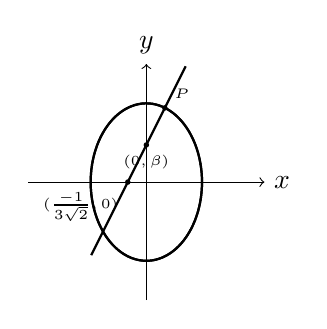
\begin{tikzpicture}
    			\draw[black, thick, domain=0:360, samples=100] 
        			plot ({sqrt(1/2)*cos(\x)}, {sin(\x)}); 
    			\draw[black, thick, domain=0:360, samples=100] 
        			plot ({sqrt(1/2)*cos(\x)}, {-sin(\x)}); 
    
    			\draw[->] (-1.5, 0) -- (1.5, 0) node[right] {$x$};
    			\draw[->] (0, -1.5) -- (0, 1.5) node[above] {$y$};
    
    
    			\draw[black, thick, domain=-0.7:0.5, samples=100]
        			plot ({\x}, {2*(\x) + 0.4714});
    
    			\fill[black] (0, 0.4714) circle (1pt) node[below] {\tiny $(0, \beta)$};
    			\fill[black] ({-1/(3*sqrt(2))}, 0) circle (1pt) node[below left] {\tiny $(\frac{-1}{3\sqrt{2}}, 0)$};
    			\fill[black] (0.235, 0.942) circle (1pt) node[above right] {\tiny $P$};		
		\end{tikzpicture}
		\end{figure}
	\item If $c$ is a point at which Rolle's Theorem holds for the function,
		\begin{align}
			f(x) = \log_e \brak{\frac{x^2 + \alpha}{7x}}
		\end{align}
		in the interval $\brak{3, 4}$, where $\alpha \in R$, then $f''(c)$ is equal to : 

		\hfill{\brak{2020-Jan}}
		\begin{enumerate}
			\begin{multicols}{4}
				\item $\frac{-1}{24}$ \columnbreak
				\item $\frac{-1}{12}$ \columnbreak
				\item $\frac{\sqrt{3}}{7}$ \columnbreak
				\item $\frac{1}{12}$
			\end{multicols}
		\end{enumerate}

	\item Let
		\begin{align}
			f\brak{x} = x \cos ^{-1}\brak{\sin \brak{-|x|}}, x \in \brak{\frac{-\pi}{2}, \frac{\pi}{2}}
		\end{align}, then which of the following is true
		
		\hfill{\brak{2020-Jan}}
		\begin{enumerate}
			\item $f\brak{0} = \frac{-\pi}{2}$ 
			\item $f'$ is decreasing in $\brak{\frac{-\pi}{2}, 0}$ and increasing in $\brak{0, \frac{\pi}{2}}$ 
			\item $f$ is not differentiable at $x = 0$  
			\item $f'$ is increasing in $\brak{\frac{-\pi}{2}, 0}$ and decreasing in $\brak{0, \frac{\pi}{2}}$
		\end{enumerate}



\iffalse
    \title{2020}
    \author{AI24BTECH11030}
    \section{mcq-single}
\fi

    \item The area (in sq. units) of the region ${\brak{x,y} \in \mathcal{R} : x^2 \leq y \leq 3 - 2x}$, is: \hfill [Jan 2020]
    \begin{multicols}{4}
    \begin{enumerate}
        \item $\frac{31}{3}$
        \item $\frac{32}{3}$
        \item $\frac{29}{3}$
        \item $\frac{34}{3}$
    \end{enumerate}
    \end{multicols}
    
    \item Let $S$ be the set of all functions $f:\sbrak{0,1} \rightarrow \mathcal{R}$, which are continuous on $\sbrak{0, 1}$ and differentiable on $\brak{0, 1}$. Then for every $f$ in $S$, there exists a $c \in \brak{0,1}$, depending on $f$, such that: \hfill [Jan 2020]
    \begin{multicols}{2}
        \begin{enumerate}
            \item $\frac{\brak{f\brak{1}-f\brak{c}}}{\brak{1-c}} = f^\prime\brak{c} $
            \item $|f\brak{c} - f\brak{1}| < |f^\prime\brak{c}| $
            \columnbreak
            \item $|f\brak{c} + f\brak{1}| < \brak{1 + c}|f ^\prime \brak{c}| $
            \item $|f\brak{c} - f\brak{1}| < \brak{1 - c}|f^\prime\brak{c}|$
        \end{enumerate}
    \end{multicols}

    \item The differential equation of the family of curves, $x^2 = 4b\brak{y + b}, b \in \mathcal{R}$, is: \hfill [Jan 2020]
    \begin{multicols}{2}
    \begin{enumerate}
        \item $xy^{\prime\prime} = y^\prime$
        \item $x\brak{y^\prime} 2 = x + 2yy^\prime$
        \columnbreak
        \item $x\brak{y ^\prime } 2 = x - 2yy^\prime$
        \item $x\brak{y ^\prime } 2 = 2yy ^\prime - x$
    \end{enumerate}
    \end{multicols}

    
    \item The system of linear equations
    \begin{align*}
        \lambda x + 2y + 2z &= 5 \\
        2\lambda x + 3y + 5z &= 8 \\
        4x + \lambda y + 6z &= 10     
    \end{align*}
    has: \hfill [Jan 2020]
    
    \begin{multicols}{2}
        \begin{enumerate}
            \item no solution when $\lambda = 2$
            \item infinitely many solutions when $\lambda = 2$
            \columnbreak
            \item no solution when $\lambda = 8$
            \item a unique solution when $\lambda = -8$
        \end{enumerate}
    \end{multicols}
    
    \item If the $10^\text{th}$ term of an A.P. is $\frac{1}{20}$ and its $20^\text{th}$ term is $\frac{1}{10}$ , then the sum of its first 200 terms is: \hfill [Jan 2020]
    \begin{multicols}{2}
        \begin{enumerate}
            \item $50 \frac{1}{4}$
            \item $100$
            \columnbreak
            \item $50$
            \item $100 \frac{1}{2}$
        \end{enumerate}
    \end{multicols}


\iffalse
    \title{2020}
    \author{EE24BTECH11011}
    \section{mcq-single}
\fi 
 
    \item If $\frac{dy}{dx} = \frac{xy}{x^2+y^2}$ and $y\brak{1}=1$, then a value of $x$ satisfying $y\brak{x}=e$ is: \hfill[2020-Jan]
    \begin{multicols}{2} % Use multicol to divide options into two columns
    \begin{enumerate}
        \item $\sqrt{3} e$\\
        \item $\frac{1}{2} \sqrt{3} e$\\
        \item $\sqrt{2}e$\\
        \item $\frac{e}{\sqrt{2}}$
    \end{enumerate}
    \end{multicols}

    % Second question
    \item If one end of focal chord $AB$ of the parabola $y^2 = 8x$ is at $A\brak{\frac{1}{2},-2}$, then the equation of the tangent at $B$ is:\hfill[2020-Jan]
    \begin{multicols}{2}
    \begin{enumerate}
        \item $x+2y+8=0$
        \item $2x-y-24=0$
        \item $x-2y+8=0$
        \item $2x+y-24=0$
    \end{enumerate}
    \end{multicols}
  \item Let $a_n$ be the $n^{th}$ term of a G.P. of positive terms. If $\sum_{n=1}^{100} a_{2n+1} = 200$ and $\sum_{n=1}^{100}a_{2n} = 100$, then $\sum_{n=1}^{200}a_n$ is equal to:\hfill[2020-Jan]
    \begin{multicols}{2}
    \begin{enumerate}
        \item $300$\\
        \item $175$
        \item $225$\\
        \item $150$
    \end{enumerate}
    \end{multicols}

\item A random variable $X$ has the following probability distribution.
    \begin{table}[h!]    
        \centering
        \begin{tabular}{|c|c|c|c|c|c|} \hline $X$ & $1$ & $2$ & $3$ & $4$ & $5$ \\ \hline P$\brak{X}$ & $K^2$ & $2K$ & $K$ & $2K$ & $5 K^2$ \\ \hline \end{tabular}
    \end{table}
    Then $P\brak{X>2}$ is:\hfill[2020-Jan]
    \begin{multicols}{2}
    \begin{enumerate}
        \item $\frac{7}{12}$\\
        \item $\frac{23}{26}$
        \item $\frac{1}{36}$\\
        \item $\frac{1}{6}$\\
    \end{enumerate}
    \end{multicols}

    % Fifth question
    \item If $\int \frac{d\theta}{\cos^2 \theta (\tan 2\theta + \sec 2 \theta)} = \lambda \tan \theta + 2 \log_e \abs {f\brak{\theta}}  + C$, where $C$ is the constant of integration, then the ordered point $\brak{\lambda, f\brak{\theta}}$ is:\hfill[2020-Jan]
    \begin{multicols}{2}
    \begin{enumerate}
        \item $\brak{-1, 1-\tan \theta}$\\
        \item $\brak{-1, 1+\tan \theta}$\\
        \item $\brak{1, 1+\tan \theta}$\\
        \item $\brak{1, 1-\tan \theta}$
    \end{enumerate}
    \end{multicols}


\iffalse
\title{02-sep-2020 shift-1}
\author{EE24BTECH11060}
\section{mcq-single}
\fi
%\begin{enumerate} [start=16]
    \item Let $\alpha$ \textgreater $0$, $\beta$\textgreater$0$ be such that $\alpha^3+\beta^3=4$.If the maximum value of the term independent of $x$ in the binomial expansion of \brak{\alpha x^\frac{1}{9}+\beta x^\frac{-1}{6}} is $10k$,then $k$ equals to:
    \hfill(sep-2020)
    \begin{enumerate}
        \item $176$
        \item $336$
        \item $352$
        \item $84$
    \end{enumerate}
    \item Let $S$ be the set of all $\lambda$ $\in$ $R$ for which the system of linear equations \\
    $2x-y+2z$=$2$\\
    $x-2y+\lambda z$=$-4$\\
    $x+\lambda y+z$=$4$ has no solution. Then the set $S$
    \hfill(sep-2020)
    \begin{enumerate}
        \item is an empty set
        \item is a singleton
        \item contains more than two elements.
        \item contains exactly two elements.
    \end{enumerate}
    \item Let $X$=$\cbrak{x\in N:1\leq x\leq 17}$ and $Y$=$\cbrak{ax+b:x \in X and a,b \in R,a \textgreater0}$.If mean and variance of elements of $Y$ are $17$ and $216$ respectively then $a+b$ is equal to:
    \hfill(sep-2020)
    \begin{enumerate}
        \item $27$
        \item $7$
        \item $-7$
        \item $9$
    \end{enumerate}
    \item Let $y$=$y\brak{x}$ be the solution of the differential equation, $\frac{2+\sin{x}}{\brak{y+1}\brak{\frac{dy}{dx}}}$=$-\cos{x}$, $y$\textgreater $0$,$y\brak{0}$=$1$.If $y\brak{\pi}$=$a$,and \brak{\frac{dy}{dx}}at $x$ = $\pi$ is $b$, then the ordered pair $\brak{a,b}$ is equal to:
    \hfill(sep-2020)
    \begin{enumerate}
        \item $\brak{2,\frac{2}{3}}$
        \item $\brak{1,1}$
        \item $\brak{2,1}$
        \item $\brak{1,-1}$
    \end{enumerate}
    \item The plane passing through the points $\brak{1,2,1}$, $\brak{2,1,2}$ and parallel to the line, $2x$ = $3y$, $z$=$1$ also passes through the point:
    \hfill(sep-2020)
    \begin{enumerate}
        \item $\brak{0,-6,2}$
        \item $\brak{0,6,-2}$
        \item $\brak{-2,0,1}$
        \item $\brak{2,0,-1}$
    \end{enumerate}
    
    
%\end{enumerate}



\iffalse
  \title{Assignment}
  \author{EE24BTECH11038}
  \section{mcq-single}
\fi  
   \item Let n be an integer. Suppose that there are n metro stations in a city located along a circular path. Each pair of stations is connected by a straight track only. Further, each pair of nearest stations is connected by blue line, whereas all remaining pairs of stations are connected by red line. If the number of red lines is 99 times the number of blue lines, then the value of n is:\hfill{Sept 2020}
   \begin{enumerate}
       \item 201
       \item 199
       \item 101
       \item 200
   \end{enumerate}
   \item If a curve y = $f\brak{x}$, passing through the point $\brak{1,2}$ is the solution of the differential equation, $2x^2dy = (2xy+y^2)dx$, then $f\brak{\frac{1}{2}}$ is equal to:\hfill{Sept 2020}
   \begin{enumerate}
       \item $-\frac{1}{1+\log_{e}^{2}}$
       \item $\frac{1}{1+\log_{e}^{2}}$
       \item ${1+\log_{e}^{2}}$
       \item $\frac{1}{1-\log_{e}^{2}}$
   \end{enumerate}
   \item  For some $\theta \in \brak{0,\frac{\pi}{2}}$ , if the eccentricity of the hyperbola, $x^2-y^2\sec ^2 \theta = 10$ is $\sqrt{5}$ times the eccentricity of the ellipse, $x^2 \sec^2 \theta+ y^2 = 5$, then the length of the latus rectum of the ellipse, is:\hfill{Sept 2020}
   \begin{enumerate}
       \item $\frac{4\sqrt{5}}{3}$
       \item $\frac{2\sqrt{5}}{3}$
       \item $2\sqrt{6}$
       \item $\sqrt{30}$
   \end{enumerate}
   \item  $\lim_{x\to 2} \brak{\tan\brak{\frac{\pi}{4}+x}}$ is equal to :\hfill{Sept 2020}
   \begin{enumerate}
       \item e
       \item $e^2$
       \item 2
       \item 1
   \end{enumerate}
   \item Let a,b,c $\in \mathbf{R}$ be all non-zero and satisfy $a^3+b^3+c^3=2$. If the matrix A=$\myvec {a & b & c \\ b & c & a \\ c & a & b}$ satisfies $A^TA=I$, then the value of abc can be \hfill{Sept 2020}
   \begin{enumerate}
       \item $\frac{2}{3}$
       \item 3
       \item $-\frac{1}{3}$
       \item $\frac{1}{3}$
   \end{enumerate}


\iffalse
\title{Assignment}
\author{K.AKSHAY TEJA}
\section{mcq-single}
\fi
\item  If $x^3dy + xydx = x^2dy + 2ydx$; $y\brak{2} = e$ and $x > 1$, then $y\brak{4}$ is equal to: \hfill \brak{Sep 2020}
        
        \begin{multicols}{4}
\begin{enumerate}
    \item $\frac{\sqrt{e}}{2}$
    \item $\frac{3}{2} \sqrt{e}$
    \item $\frac{1}{2} + \sqrt{e}$
    \item $\frac{3}{2} + \sqrt{e}$
\end{enumerate}
\end{multicols}

%2
\item Let $A$ be a $3 \times 3$ matrix such that adj $A = \begin{bmatrix}
2 &-1& 1\\-1& 0& 2\\1& -2& -1
\end{bmatrix} $
and $B =$ adj$\brak{adj  A}$. If $\abs{A} = \lambda$ and $\abs{\brak{B^{-1}}^T} = \mu$, then the ordered pair, $\brak{\abs{\lambda}, \mu}$ is equal to:
 \hfill \brak{Sep 2020}

          \begin{multicols}{4}

\begin{enumerate}
    \item $\brak{9, \frac{1}{81}}$
    \item $\brak{9, \frac{1}{9}}$
    \item $\brak{3, \frac{1}{81}}$
    \item $\brak{3, 81}$
\end{enumerate}
\end{multicols}

%3
\item Let $a, b, c \in R$ be such that $a^2 + b^2 + c^2 = 1$, if $a \cos \theta = b \cos\brak{\theta + \frac{2\pi}{3}} = c \cos\brak{\theta + \frac{4\pi}{3}}$, where $\theta = \frac{\pi}{9}$, then the angle between the vectors $a\hat{i} + b\hat{j} + c\hat{k}$ and $b\hat{i} + c\hat{j}+ a\hat{k} $ is: \hfill \brak{Sep 2020}

        \begin{multicols}{4}

\begin{enumerate}
    \item $\frac{\pi}{2}$
    \item $\frac{2\pi}{3}$
    \item $\frac{\pi}{9}$
    \item $0$
\end{enumerate}
\end{multicols}

%4
\item Suppose $f\brak{x}$ is a polynomial of degree four, having critical points at $\brak{-1, 0, 1}$. If $T = \{ x \in R \mid f\brak{x} = f\brak{0} \}$, then the sum of squares of all the elements of $T$ is: \hfill \brak{Sep 2020}

        \begin{multicols}{4}

\begin{enumerate}
    \item 6
    \item 2
    \item 8
    \item 4
\end{enumerate}
\end{multicols}

%5
\item If the value of the integral $ \int_{0}^{\frac{1}{2}} \frac{x^2}{\brak{1 - x^2}^{\frac{3}{2}}}$ is $\frac{k}{6}$, then $k$ is equal to: \hfill \brak{Sep 2020}

        
          \begin{multicols}{4}
\begin{enumerate}
    \item $2\sqrt{3} + \pi$
    \item $3\sqrt{2} + \pi$
    \item $3\sqrt{2} - \pi$
    \item $2\sqrt{3} - \pi$
\end{enumerate}
\end{multicols}

%6
 \item If the term independent of $x$ in the expansion of $\brak{ \brak{ \frac{3}{2} } x^2 - \frac{1}{3x} }^9$ is $k$, then $18k$ is equal to:  \hfill \brak{Sep 2020}

        \begin{multicols}{4}

\begin{enumerate}
    \item 5
    \item 9
    \item 7
    \item 11
\end{enumerate}
\end{multicols}

%7
\item If a triangle $ABC$ has vertices $A\brak{-1, 7}$, $B\brak{-7, 1}$, and $C\brak{5, -5}$, then its orthocentre has coordinates:  \hfill \brak{Sep 2020}

          \begin{multicols}{4}

\begin{enumerate}
    \item $\brak{-3, 3}$
    \item $\brak{-\frac{3}{5}, \frac{3}{5}}$
    \item $\brak{\frac{3}{5}, -\frac{3}{5}}$
    \item $\brak{3, -3}$
\end{enumerate}
\end{multicols}

%8
\item  Let $e_1$ and $e_2$ be the eccentricities of the ellipse, $\frac{x^2}{25} + \frac{y^2}{b^2} = 1$ $\brak{where b < 5}$ and the hyperbola, $\frac{x^2}{16} - \frac{y^2}{b^2} = 1$ respectively, satisfying $e_1 e_2 = 1$. If $\alpha$ and $\beta$ are the distances between the foci of the ellipse and the foci of the hyperbola respectively, then the ordered pair $\brak{\alpha, \beta}$ is equal to:  \hfill \brak{Sep 2020}

          \begin{multicols}{4}

\begin{enumerate}
    \item $\brak{8, 12}$
    \item $\brak{\frac{24}{5}, 10}$
    \item $\brak{\frac{20}{3}, 12}$
    \item $\brak{8, 10}$
\end{enumerate}
\end{multicols}

%9
\item If $z_1, z_2$ are complex numbers such that Re$\brak{z_1} = \abs{z_1 - 1}$, Re$\brak{z_2} = \abs{z_2 - 1}$ and $\arg\brak{z_1 - z_2} = \frac{\pi}{6}$, then Im$\brak{z_1 + z_2}$ is equal to: \hfill \brak{Sep 2020}

        \begin{multicols}{4}

\begin{enumerate}
    \item $2\sqrt{3}$
    \item $\frac{2}{\sqrt{3}}$
    \item $\frac{1}{\sqrt{3}}$
    \item $\frac{\sqrt{3}}{2}$
\end{enumerate}
\end{multicols}

%10
\item The set of all real values of $\lambda$ for which the quadratic equations, $\brak{\lambda^2 + 1}x^2 - 4\lambda x + 2 = 0$ always have exactly one root in the interval $\brak{0, 1}$ is: \hfill \brak{Sep 2020}

        
          \begin{multicols}{4}
\begin{enumerate}
    \item $\brak{-3, -1}$
    \item $\brak{2, 4}$
    \item $\brak{1, 3}$
    \item $\brak{0, 2}$
\end{enumerate}
\end{multicols}

%11
\item Let the latus rectum of the parabola $y^2 = 4x$ be the common chord to the circles $C_1$ and $C_2$, each of them having radius $2\sqrt{5}$. Then, the distance between the centres of the circles $C_1$ and $C_2$ is: \hfill \brak{Sep 2020}


\begin{multicols}{4}
\begin{enumerate}
    \item $8$
    \item $8\sqrt{5}$
    \item $4\sqrt{5}$
    \item $12$
\end{enumerate}
\end{multicols}

%12
\item The plane which bisects the line joining the points $\brak{4, -2, 3}$ and $\brak{2, 4, -1}$ at right angles also passes through the point:  \hfill \brak{Sep 2020}


  \begin{multicols}{4}
\begin{enumerate}
    \item $\brak{0, -1, 1}$
    \item $\brak{4, 0, 1}$
    \item $\brak{4, 0, -1}$
    \item $\brak{0, 1, -1}$
\end{enumerate}
\end{multicols}

%13
\item $\lim_{x \to a} \frac{\brak{a + 2x}^{\frac{1}{3}} - \brak{3x}^{\frac{1}{3}}}{\brak{3a + x}^{\frac{1}{3}} - \brak{4a}^{\frac{1}{3}}}$ is equal to:  \hfill \brak{Sep 2020}

  \begin{multicols}{4}
\begin{enumerate}
    \item $\frac{2}{9} \brak{\frac{4}{3}}$
    \item $\frac{2}{3} \brak{\frac{4}{3}}$
    \item $\brak{\frac{2}{3}} \brak{\frac{2}{9}}^{\frac{1}{3}}$
    \item $\brak{\frac{2}{9}} \brak{\frac{2}{3}}^{\frac{1}{3}}$
\end{enumerate}
\end{multicols}

%14
\item Let $x_{i} \brak{1 \leq i \leq 10}$ be ten observations of a random variable $X$. If
$\sum_{i=1}^{10}\brak{x_{i}-p}=3$
and
$\sum_{i=1}^{10}\brak{x_{i}-p}^{2}=9$
where $0 \neq p \in R$, then the standard deviation of these observations is:  \hfill \brak{Sep 2020}

\begin{multicols}{4}
\begin{enumerate}
    \item  $\frac{7}{10}$
    \item $\frac{9}{10}$
    \item $\sqrt{\frac{3}{5}}$
    \item  $\frac{4}{5}$
\end{enumerate}
\end{multicols}

%15
\item  The probability that a randomly chosen 5-digit number is made from exactly two digits is: \hfill \brak{Sep 2020}

\begin{multicols}{4}
\begin{enumerate}
    \item $\frac{134}{10^4}$
    \item $\frac{121}{10^4}$
    \item $\frac{135}{10^4}$
    \item $\frac{50}{10^4}$
\end{enumerate}
\end{multicols}

%\end{enumerate}
%\end{document}




\iffalse
  \title{Assignment 4}
  \author{AI24BTECH11014}
  \section{mcq-single}
\fi


%\begin{enumerate}                     
\item If $x=1$ is a critical point of the function $f\brak{x} = \brak{3x^{2}+ax-2-a}e^{x}$, then: 
	\hfill{Sep 2020} 
\begin{enumerate}                            
\item $x=1$ is a local minima and $x = -\frac{2}{3}$ is a local maxima of $f$.          
\item $x=1$ is a local maxima and $x=-\frac{2}{3}$ is a local minima of $f$.            
\item $x=1$ and $x=-\frac{2}{3}$ are local minima of $f$.           
\item $x=1$ and $x=-\frac{2}{3}$ are local maxima of $f$.       
\end{enumerate}
\item
	  \begin{align}
		  \lim_{x \to 0}\frac{x\brak{{e}^{\frac{\sqrt{1+x^{2}+x^{4}} - 1}{x}} -1 }}{\sqrt{1+x^{2}+x^{4}} - 1}
	  \end{align}
		\hfill{Sep 2020}
\begin{enumerate}
  \begin{multicols}{4}
  \item  is equal to $\sqrt{e}$
  \item is equal to $1$
  \item is equal to $0$
  \item does not exist
  \end{multicols}
  \end{enumerate}
 \item The statement $(p \rightarrow (q \rightarrow p)) \rightarrow (p \rightarrow (p \cup q))$ is:
	 \hfill{Sep 2020}
  \begin{enumerate}
 \item equivalent to $\brak{p \cup q} \cap \brak{ \sim p}$       
 \item equivalent to $\brak{p \cap q} \cup \brak{ \sim p}$      
 \item a contradiction
  \item a tautology
  \end{enumerate}
  \item If $L = \sin^2\left(\frac{\pi}{16}\right) - \sin^2\left(\frac{\pi}{8}\right)$
 and $M = \cos^2\left(\frac{\pi}{8}\right) - \sin^2\left(\frac{\pi}{8}\right)$, then:  
		\hfill{Sep 2020}
 \begin{enumerate}  
		 \begin{multicols}{2}
 \item $M = \frac{1}{2\sqrt{2}}+\frac{1}{2}\cos\frac{\pi}{8}$      
 \item $M = \frac{1}{4\sqrt{2}}+\frac{1}{4}\cos\frac{\pi}{8}$    
 \item $L = -\frac{1}{2\sqrt{2}}+\frac{1}{2}\cos\frac{\pi}{8}$    
		 \item $L=\frac{1}{4\sqrt{2}}-\frac{1}{4}\cos\frac{\pi}{8}$                         \end{multicols}    
 \end{enumerate}
 \item If the sum of the first $20$ terms of the series $\log_{{7}^{\frac{1}{2}}} x + \log_{{7}^{\frac{1}{3}}} x + \log_{{7}^{\frac{1}{4}}} x + \dots$ is $460$, then $x$ is equal to:
	 \hfill{Sep 2020}
 \begin{enumerate}
 \begin{multicols}{4}
 \item ${7}^{\frac{1}{2}}$
 \item ${7}^{2}$
 \item ${e}^{2}$
\item ${7}^{\frac{46}{21}}$
 \end{multicols}
 \end{enumerate} 
 \item There are $3$ sections in a question paper and each section contains $5$ questions candidate has to answer a total of $5$ questions, choosing at least one question from each section. Then the number of ways, in which the candidate can choose the questions, is:
	 \hfill{Sep 2020}
 \begin{enumerate}
 \begin{multicols}{4}
     \item $2250$
     \item $2255$
     \item $1500$
     \item $3000$
\end{multicols}
     \end{enumerate}
     \item If the mean and the standard deviation of the data $3,5,7,a,b$ are $5$ and $2$ respectively, then $a$ and $b$ are the roots of the equation:
	     \hfill{Sep 2020}
     \begin{enumerate}
    \begin{multicols}{2}
\item $x^{2}-20x+18=0$
\item $x^{2}-10x+19=0$
\item $2x^{2}-20+19=0$
\item $x^{2}-10x+18=0$
     \end{multicols}
     \end{enumerate}
     \item The derivative of $\tan^{-1}\brak{\frac{\sqrt{1+x^{2}}-1}{x}}$ with respect to $\tan^{-1}\brak{\frac{2x\sqrt{1-x^{2}}}{1-2x^{2}}}$ at $x=\frac{1}{2}$ is:
	     \hfill{Sep 2020}
     \begin{enumerate}
     \begin{multicols}{4}
     \item $\frac{ 2 \sqrt{3}}{3}$
     \item $\frac{2\sqrt{3}}{5}$
     \item $\frac{\sqrt{3}}{12}$
     \item $\frac{\sqrt{3}}{10}$
     \end{multicols}
      \end{enumerate}
      \item If 
	      \begin{align}
		      \int \frac{\cos\theta}{5+7\sin\theta-2\cos^{2}\theta}d\theta= A\log_{e}|B\brak{\theta}|+C
	      \end{align}
	      where C is a constant of integration, then $\frac{B\brak{\theta}}{A}$ can be:
	      \hfill{Sep 2020}
      \begin{enumerate}
      \begin{multicols}{4}
      \item $\frac{5\brak{2\sin\theta+1}}{\sin\theta+3}$
      \item $\frac{5\brak{\sin\theta+3}}{2\sin\theta+1}$
       \item $\frac{2\sin\theta+1}{\sin\theta+3}$
       \item $\frac{2\sin\theta+1}{5\brak{\sin\theta+3}}$
      \end{multicols}
      \end{enumerate}
      \item If the length of the cord of the circle, $x^{2}+y^{2}=r^{2}\brak{r>0}$ along the line, $y-2x=3$ is $r$, then $r^{2}$ is equal to:
	      \hfill{Sep 2020}
      \begin{enumerate}
      \begin{multicols}{4}
      \item $12$
      \item $\frac{24}{5}$
      \item $\frac{9}{5}$
      \item $\frac{12}{5}$
      \end{multicols}
      \end{enumerate}
      \item If $\alpha$ and $\beta$ are the roots of the equation, $7x^{2}-3x-2=0$, then the value of$\frac{\alpha}{1-\alpha^{2}} +\frac{\beta}{1-\beta^{2}}$
	      \hfill{Sep 2020}
      \begin{enumerate}
      \begin{multicols}{4}
      \item $\frac{27}{32}$
      \item $\frac{1}{24}$
      \item $\frac{27}{16}$
      \item $\frac{3}{8}$
      \end{multicols}
      \end{enumerate}
      \item If the sum of the second, third and fourth terms of a positive term G.P. is $3$ and the sum of its sixth, seventh and eighth terms is $243$, then the sum of the first $50$ terms of the G.P. is:
	      \hfill{Sep 2020}
       \begin{enumerate}
      \begin{multicols}{4}
      \item $\frac{2}{13}\brak{3^{50}-1}$
      \item $\frac{1}{26}\brak{3^{49}-1}$
      \item $\frac{1}{13}\brak{3^{50}-1}$\item $\frac{1}{26}\brak{3^{50}-1}$
      \end{multicols}
      \end{enumerate}
     \item If the line $y=mx+c$ is a common tangent to the hyperbola $\frac{x^{2}}{100} - \frac{y^{2}}{64}=1$ and the circle $x^{2}+y^{2}=36$, then which one of the following is true?
	     \hfill{Sep 2020}
      \begin{enumerate}
      \begin{multicols}{4}
      \item $4c^{2}=369$
      \item $c^{2}=369$
      \item $8m+5=0$
      \item $5m=4$
      \end{multicols}
      \end{enumerate}
      \item The area (in sq.units) of the region 
	      \begin{align}
		      A = \cbrak{\brak{x,y}:\brak{x-1} \sbrak{x} \leq y \leq 2\sqrt{x}, 0\leq x\leq 2}
	      \end{align}
	      where $\sbrak{t}$ denotes the greatest integer function, is:
	      \hfill{Sep 2020}
      \begin{enumerate}
      \begin{multicols}{4}
      \item $\frac{4}{3}\sqrt{2}-\frac{1}{2}$
      \item $\frac{8}{3}\sqrt{2}-\frac{1}{2}$
      \item $\frac{8}{3}\sqrt{2}-1$
      \item $\frac{4}{3}\sqrt{2}+1$
      \end{multicols}
      \end{enumerate}
     \item If $a+x=b+y=c+z+1$, where $a, b, c, x, y, z$ are non-zero distinct real numbers, then  
    $\left| \begin{matrix} x & a+y & x+a \\ y & b+y & y+b \\z & c+y & z+c  \end{matrix} \right|$ is equal to:
	    \hfill{Sep 2020}
     \begin{enumerate}
      \begin{multicols}{4}
      \item $y\brak{a-b}$
      \item $0$
      \item $y\brak{b-a}$
      \item $y\brak{a-c}$
       \end{multicols}
      \end{enumerate}

      
 %\end{enumerate}
 %\end{document}

\iffalse
    \title{2020}
    \author{AI24BTECH11030}
    \section{mcq-single}
\fi

    \item $\lim_{x \rightarrow 1} \brak{\frac{\int_{0}^{\brak{x-1}^2} t \cos \brak{t^2} dt}{\brak{x-1}\sin\brak{x-1}}}$ \hfill [Sep 2020]
    
    \begin{multicols}{4}
    \begin{enumerate}
        \item is equal to $1$
        \item is equal to $\frac{1}{2}$
        \item does not exist
        \item is equal to $\frac{-1}{2}$
    \end{enumerate}
    \end{multicols}
    
    \item If $\sum_{i=1}^{n}(x_i - a) = n$ and $\sum_{i=1}^{n} (x_i - a)^2 = na$, $(n,a >1)$ then the standard deviation of $n$ observations $x_1, x_2, x_3\ldots x_n$ is: \hfill [Sep 2020]
    
    \begin{multicols}{4}
    \begin{enumerate}
        \item $nv(a-1)$
        \item $v(na-1)$
        \item $a-1$
        \item $v(a-1)$
    \end{enumerate}
    \end{multicols}
    
    \item If $\alpha$ and $\beta$ be two roots of the equation $x^2 -64x+256 = 0$. Then the value of $(\frac{\alpha^3}{\beta^5})^\frac{1}{8}+(\frac{\beta^3}{\alpha^5})^\frac{1}{8}$ is: \hfill [Sep 2020]

    \begin{multicols}{4}
    \begin{enumerate}
        \item $1$
        \item $3$
        \item $2$
        \item $4$
    \end{enumerate}
    \end{multicols}
    
    \item The position of a moving car at time $t$ is given by $f(t) = at^2+bt+c, t > 0$, where $a$, $b$ and $c$ are real numbers greater than 1. Then the average speed of the car over the time interval $\sbrak{t_1, t_2}$ is attained at the point \hfill [Sep 2020]

    \begin{multicols}{4}
    \begin{enumerate}
        \item $\frac{(t_1+t_2)}{2}$
        \item $2a(t_1+t_2)+b$
        \item $\frac{(t_2-t_1)}{2}$
        \item $a(t_2-t_1)+b$
    \end{enumerate}
    \end{multicols}
    
    \item If $I_1 = \int_{0}^{1}(1-x^{50})^{100} dx$ and $I_2 = \int_{0}^{1}(1-x^{50})^{101} dx$ such that $I_2 = \alpha I_1$ then $\alpha$ equals to \hfill [Sep 2020]
    
    \begin{multicols}{4}
    \begin{enumerate}
        \item $\frac{5050}{5049}$
        \item $\frac{5050}{5051}$
        \item $\frac{5051}{5050}$
        \item $\frac{5049}{5050}$
    \end{enumerate}
    \end{multicols}
    

\iffalse
\title{Assignment}
\author{ee24btech11059}
\section{mcq-single}
\fi

    \item{
          	If the normal at an end of a latus rectum of an ellipse passes through an extremity of the minor axis, then the eccentricity e of the ellipse satisfies: \\ \text{  }\hfill
                {[Sep 2020]}
            \begin{multicols}{2}
				\begin{enumerate}
					\item $e^4+2e^2 - 1 = 0$
					\item $e^2+2e - 1 = 0$
					\item $e^4+e^2 - 1 = 0$
					\item $e^2+e - 1 = 0$
				\end{enumerate}
			\end{multicols}
            }
    %code by ysiddhanth 
    \item{
            The set of all real values of $\lambda$ for which the function $f\brak{x} = \brak{1- \cos^2 x}\brak{\lambda+\sin x} , x\in\brak{-\frac{\pi}{2}, \frac{\pi}{2}}$, has exactly one maxima and exactly one minima, is:\hfill
                {[Sep 2020]}
            \begin{multicols}{2}
                \begin{enumerate}
                    \item $\brak{-\frac{3}{2}, \frac{3}{2}}-\cbrak{0}$
                    \item $\brak{-\frac{1}{2}, \frac{1}{2}}-\cbrak{0}$
                    \item $\brak{-\frac{3}{2}, \frac{3}{2}}$
                    \item $\brak{-\frac{1}{2}, \frac{1}{2}}$
                \end{enumerate}
            \end{multicols}
        }
\item{
        	
        	The probabilities of three events $A$, $B$ and $C$ are given by $P\brak{A} = 0.6$, $P\brak{B} = 0.4$ and $P\brak{C} = 0.5$. If $P\brak{A \cup B} = 0.8$, $P\brak{A \cap C} = 0.3$, $P\brak{A \cap B \cap C} = 0.2$, $P\brak{B \cap C} = \beta$ and $P\brak{A \cup B \cup C} = \alpha$, where $0.85 \leq \alpha \leq 0.95$, then $\beta$ lies in the interval. \\
        	\hfill
        	{[Sep 2020]}
        	\begin{multicols}{4}
        		\begin{enumerate}
        			\item $\sbrak{0.36,0.40}$
        			\item $\sbrak{0.25,0.35}$
        			\item $\sbrak{0.35,0.36}$
        			\item $\sbrak{0.20,0.25}$
        		\end{enumerate}
        	\end{multicols}
        	
        }
    \item{
     
            The common difference of the $A.P.$ $b_1, b_2, \ldots, b_m$ is $2$ more than the common difference of $A.P.$ $a_1, a_2, \ldots, a_n$. If $a_{40} = -159$, $a_{100} = -399$ and $b_{100} = a_{70}$, then $b_1$ is equal to:\hfill
                {[Sep 2020]}
            \begin{multicols}{4}
                \begin{enumerate}
                    \item -127
                    \item 81
                    \item 127
                    \item -81
                \end{enumerate}
            \end{multicols}
        
        }
    \item{
            The integral $\int_{1}^{2}e^{x}.x^{x}\brak{2+log_{e}x}dx$ equals
           	\hfill
                {[Sep 2020]}
            
            \begin{multicols}{2}
				\begin{enumerate}
					\item $e\brak{4e-1}$
					\item $e\brak{4e+1}$
					\item $4e^2-1$
					\item $e\brak{2e-1}$
				\end{enumerate}
			\end{multicols}
        
        }
 	\item{
        	If the tangent to the curve, $y = f(x) = x\log_e x$, $\brak{x>0}$ at a point $\brak{c,f\brak{c}}$ is parallel to the line-segment joining the points $\brak{1,0}$ and $\brak{e,e}$, then $c$ is equal to: \\ \text{ }
        	\hfill
        	{[Sep 2020]}
        	
        	\begin{multicols}{4}
        		\begin{enumerate}
					\item \( e^{\brak{\frac{1}{1-e}}} \)
					\item \( \frac{\brak{e-1}}{e} \)
					\item \( \frac{1}{\brak{e-1}} \)
					\item \( e^{\brak{\frac{1}{e-1}}} \)
        		\end{enumerate}
        	\end{multicols}
        	
        }
 	\item{
			If $y = \brak{\frac{2}{\pi}x-1} \csc x$ is the solution of the differential equation, $\brak{\frac{dy}{dx}}+p\brak{x}y = \brak{\frac{2}{\pi}-1}\csc x$, $0<x<\frac{\pi}{2}$, then the function $p\brak{x}$ is equal to: 
			\hfill
			{[Sep 2020]}
			
			\begin{multicols}{4}
				\begin{enumerate}
					\item $\cosec x$
					\item $\cot x$
					\item $\tan x$
					\item $\sec x$
				\end{enumerate}
			\end{multicols}
			
		}
 	\item{
			If $\alpha$ and $\beta$ are the roots of the equation $2x\brak{2x+1} = 1$, then $\beta$ is equal to:\\ \text{ }
			\hfill
			{[Sep 2020]}
			
			\begin{multicols}{2}
				\begin{enumerate}
					\item $2\alpha\brak{\alpha-1}$
					\item $-2\alpha\brak{\alpha+1}$
					\item $2\alpha^2$
					\item $2\alpha\brak{\alpha+1}$
				\end{enumerate}
			\end{multicols}
			
		}
    \item{
            For all twice differentiable functions \( f: \mathbb{R} \to \mathbb{R} \), with \( f\brak{0} = f\brak{1} = f^{\prime}\brak{0} = 0 \), \\ \text{ }
             \hfill
                {[Sep 2020]}
            \begin{multicols}{2}
                \begin{enumerate}
                    \item $f^{\prime\prime}\brak{x} = 0$, at every point $x \in \brak{0,1}$
                    \item $f^{\prime\prime}\brak{x} \neq 0$, at every point $x \in \brak{0,1}$
                    \item $f^{\prime\prime}\brak{x} = 0$, for some $x \in \brak{0,1}$
                    \item $f^{\prime\prime}\brak{0} = 0$
                \end{enumerate}
            \end{multicols}

        %code by ysiddhanth 
        
        }
    \item{
            The area (in sq.units) of the region enclosed by the curves $y = x^2-1$ and $y = 1-x^2$ is equal to:
             \hfill
                {[Sep 2020]}
            \begin{multicols}{4}
                \begin{enumerate}
                    \item $\frac{4}{3}$
                   	\item $\frac{7}{2}$
                   	\item $\frac{16}{3}$
                    \item $\frac{8}{3}$
                \end{enumerate}
            \end{multicols}
        
        }
    \item{
            For a suitably chosen real constant $a$, let a function, $f: \mathbb{R} - \cbrak{-a} \rightarrow \mathbb{R}$ be defined by $f\brak{x} = \frac{a-x}{a+x}$. Further suppose that for any real number $x \neq -a$ and $f\brak{x} \neq -a$, $\brak{f \circ f}\brak{x} = x$. Then $f\brak{\frac{-1}{2}}$ is equal to:
             \hfill
                {[Sep 2020]}
			\begin{multicols}{4}
				\begin{enumerate}
					\item -3
					\item 3
					\item $\frac{1}{3}$
					\item $-\frac{1}{3}$
				\end{enumerate}
			\end{multicols}
        
        }
    \item{
        
            Let $\theta = \frac{\pi}{5}$ and $A = \myvec{ \cos\theta & -\sin\theta \\ \sin\theta & \cos\theta}$. If $B = A + A^4$, then $\det(B)$:
             \text{   }\hfill
                {[Sep 2020]}
            \begin{multicols}{2}
                \begin{enumerate}
                   	\item is one
                    \item lies in \brak{1,2}
                    \item lies in \brak{2,3}
                    \item is zero
                \end{enumerate}
            \end{multicols}
        
        }
    \item{
	
			The center of the circle passing through the point $\brak{0,1}$ and touching the parabola $y=x^2$ at the point $\brak{2,4}$ is :
			\text{   }\hfill
			{[Sep 2020]}
			\begin{multicols}{4}
				\begin{enumerate}
					\item $\brak{\frac{3}{10}, \frac{16}{5}}$
					\item $\brak{\frac{6}{5}, \frac{53}{10}}$
					\item $\brak{-\frac{16}{5}, \frac{53}{10}}$
					\item $\brak{-\frac{53}{10}, \frac{16}{5}}$
				\end{enumerate}
			\end{multicols}
			
		}
    \item{
	
			A plane $P$ meets the coordinate axes at $A$, $B$ and $C$ respectively. The centroid of a triangle $ABC$ is given to be $\brak{1,1,2}$. Then the equation of the line through this centroid and perpendicular to the plane $P$ is:
			\text{   }\hfill
			{[Sep 2020]}
			\begin{multicols}{2}
				\begin{enumerate}
					\item $\frac{x-1}{2} = \frac{y-1}{1} = \frac{z-2}{1}$
					
					\item $\frac{x-1}{2} = \frac{y-1}{2} = \frac{z-2}{1}$
					
					\item $\frac{x-1}{1} = \frac{y-1}{2} = \frac{z-2}{2}$
					
					\item $\frac{x-1}{1} = \frac{y-1}{1} = \frac{z-2}{2}$
				\end{enumerate}
			\end{multicols}
			
		}
    \item{
        
            Let $f : \mathbb{R}\rightarrow \mathbb{R}$ be a function defined by $f(x) = \max \cbrak{x,x^2}$. Let $S$ denote the set of all points in $\mathbb{R}$, where $f$ is not differentiable. Then
             \hfill
              {[Sep 2020]}
              \begin{multicols}{2}
              	\begin{enumerate}
              		\item $\cbrak{0,1}$
              		\item an empty set
              		\item $\cbrak{1}$
              		\item $\cbrak{0}$
              	\end{enumerate}
              \end{multicols}
        
        }





\end{enumerate}
\subsection*{Integer Value Type Questions}
\begin{enumerate}[label=\thechapter.\arabic*,ref=\thechapter.\theenumi]

\iffalse
    \title{2020}
    \author{EE24BTECH11001}
    \section{integer}
\fi 
\item An urn contains 5 red marbles, 4 black marbles and 3 white marbles. Then the number of ways in which 4
	marbles can be drawn so that at most three of the are red is.
		\hfill{\brak{2020-Jan}}
\\
	\item Let the normal at a point $P$ on the curve $y^2 - 3x^2 + y + 10 = 0$ intersect the y-axis at 
		$\brak{0, \frac{3}{2}}$. If $m$ is the slope of the tangent at $P$ to the curve, te $\abs{m}$ is equal to
		\hfill{\brak{2020-Jan}}
		\begin{figure}[ht]
		\centering
		\begin{tikzpicture}
   			\draw[black, thick] (-5, 0) -- (5, 0) node[right] {$x$};
			\draw[black, thick] (0, -5) -- (0, 5) node[above] {$y$};
			\draw[domain=-3.5:-1.8027757,smooth,variable=\x,black] plot ({\x},{(-1 + sqrt(1 + 12*(\x)^2 - 40))/2});
			\draw[domain=-3.5:-1.8027757,smooth,variable=\x,black] plot ({\x},{(-1 - sqrt(1 + 12*(\x)^2 - 40))/2});
			\draw[domain=1.8027757:3.5,smooth,variable=\x,black] plot ({\x},{(-1 + sqrt(1 + 12*(\x)^2 - 40))/2});
			\draw[domain=1.8027757:3.5,smooth,variable=\x,black] plot ({\x},{(-1 - sqrt(1 + 12*(\x)^2 - 40))/2});
    			\draw[black, thick, domain=0.5:3, samples=100]
				plot ({\x}, {4 * (\x) - 7});
    			\draw[black, thick, domain=-3:6, samples=100]
				plot ({\x}, {-0.25 * (\x) + 1.5});
    			\fill[black] (2, 1) circle (3pt) node[left] {\small $(2, 1)$};
			\fill[black] (0, 1.5) circle (3pt) node[above] {\small $(0, \frac{3}{2})$};
		\end{tikzpicture}
		\end{figure}
\\	
	\item The least positive value of $'a'$ for which the equation
	\begin{align}
		2x^2 + \brak{a - 10}x + \frac{33}{2} = 2a
	\end{align} has real roots is
		\hfill{\brak{2020-Jan}}
\\
	\item The sum
	\begin{align}
		\sum_{k = 1}^{20} \brak{1 + 2 + 3 + \dots + k}
	\end{align} is
		\hfill{\brak{2020-Jan}}
\\
	\item The number of all 3 $\times$ 3 matrices $A$, with entries from the set $\{-1, 0 , 1\}$, such that the sum
	of the diagonal elements of $\brak{AA^\top}$ is 3, is
		\hfill{\brak{2020-Jan}}
	



\iffalse
    \title{2020}
    \author{AI24BTECH11030}
    \section{integer}
\fi


    \item Let a line $y = mx \: \brak{m > 0}$ intersect the parabola, $y^2 = x$ at a point $P$, other than the origin. Let the tangent to it at $P$ meet the x-axis at the point $Q$. If $area\brak{\Delta OPQ} = 4 \text{ sq.units}$, then $m$ is equal to $\ldots$ \hfill [Jan 2020]\\
    
    \item Let $f\brak{x}$ be a polynomial of degree 3 such that $f\brak{-1} = 10$, $f\brak{1} = -6$, $f\brak{x}$ has a critical point at $x = -1$ and $f^\prime\brak{x}$ has a critical point at $x = 1$. Then the local minima at $x$ = $\ldots$ \hfill [Jan 2020]\\
    
    \item $\frac{\sqrt{2}\sin\alpha}{\sqrt{1 + \cos2\alpha}} = \frac{1}{7}$ and $\sqrt{\frac{1-\cos2\beta}{2}} = \frac{1}{\sqrt{10}}$, $\alpha, \beta \in \brak{0, \frac{\pi}{2}}$, then $\tan\brak{\alpha + 2\beta}$ is equal to $\ldots$ \hfill [Jan 2020]\\
    
    \item The number of 4 letter words (with or without meaning) that can be made from the eleven letters of the word ``EXAMINATION'' is $\ldots$ \hfill [Jan 2020]\\
    
    \item The sum, $\sum_{n=1}^{7}\frac{n\brak{n+1}\brak{2n+1}}{4}$ is equal to $\ldots$ \hfill [Jan 2020]\\
\iffalse
    \title{2020}
    \author{EE24BTECH11011}
    \section{integer}
\fi 
 \item Let $\Vec{a}$, $\vec{b}$, and $\vec{c}$ be three vectors such that $\abs{\vec{ a}}=3$ , $\abs{\vec {b}}=5$ ,$\vec{a}\cdot \vec{b}= 10$ and the angle between $\vec{b}$ and $\vec{c}$ is $\frac{\pi}{3}$. If $\vec{a}$ is perpendicular to vector $\vec{b} \times \vec{c}$ ,  then $\abs{\vec{a} \times \brak{\vec{b}\times \vec{c}}}$ is equal to \rule{1cm}{0.15mm} \hfill[2020-Jan]\\

   \item If $\comb{}{r} = \comb{25}{r}$ and $\comb{}{0}+ 5 \cdot \comb{}{1}+ 9 \cdot \comb{}{2}+ \dots + 101 \cdot \comb{}{25} = 2^{25}. k $ then $k$ is equal to \rule{1cm}{0.15mm}\hfill[2020-Jan] \\


   \item If the curves $x^2-6x+y^2+8=0$ and $x^2-8y+y^2+16-k=0$ , $\brak{k>0}$ touch each other at a point , then the largest value of $k$ is \rule{1cm}{0.15mm}\hfill[2020-Jan] \\

   \item The number of terms common to the A.P.'s $3,7,11,\dots , 407$ and $2,9,16,\dots , 709$ is \rule{1cm}{0.15mm}\hfill[2020-Jan] \\


   \item If the distance between the plane , $23x-10y-2z+48=0$ and the plane containing the lines $\frac{x+1}{2} = \frac{y-3}{4} = \frac{z+1}{3}$ and $\frac{x+3}{2} = \frac{y+2}{6} = \frac{z-1}{\lambda}$ , $\brak{\lambda \in R}$ is equal to $\frac{k}{\sqrt{633}}$ the $k$ is equal to \rule{1cm}{0.15mm}\hfill[2020-Jan] \\



\iffalse
\title{02-sep-2020 shift-1}
\author{ee24btech11060}
\section{integer}
\fi
%\begin{enumerate}
\item  The number of integral values of $k$ for which the line, $3x+4y$ = $k$ intersects the circle, $x^2+y^2-2x-4y+4$=$0$ at two distinct points is
    \hfill(sep-2020)
    \item Let $\Vec{a},\Vec{b}$ and $\Vec{c}$ be three unit vectors such that $\abs{a-b}^2+\abs{a-c}^2=8$.Then $\abs{a+2b}^2+\abs{a+2c}^2$ is equal to:
    \hfill(sep-2020)
    \item If the letters of the word MOTHER be permuted and all the words so formed  be listed as in a dictionary, then the position of the word MOTHER is \dots 
    \hfill(sep-2020)
    \item  If $\lim_{x \to 1}$ $\frac{x+x^2+x^3+\dots x^n-n}{x-1}$=$820$ $n$ $\in$ $N$, then the value of $n$ is equal to: \\
    \hfill(sep-2020)
    \item The integral $\int_{0}^{2} \abs{\abs{x-1}-x}dx$ is equal to:
    \hfill(sep-2020)
%\end{enumerate}    

\iffalse
  \title{Assignment}
  \author{EE24BTECH11038}
  \section{integer}
\fi  
\item Let the position vectors of points `$\vec{A}$' and `$\vec{B}$' be $\hat{i} +\hat{j}+\hat{k}$ and $2\hat{i} +\hat{j}+3\hat{k}$ respectively. A point `$\vec{P}$' divides the line segment AB internally in the ratio $\lambda$:1 $\brak{\lambda > 0}$ . If $\vec{O}$ is the origin and $\vec{OB}$.$\vec{OP}$ -3$\abs{\vec{OA}\,X\,\vec{OP}}^2$=6 then $\lambda$ is :\hfill{sept 2020}
   \item Let $\sbrak{t}$ denote the greatest integer less than or equal to t. Then the value of
   $\int_{1}^{2}\abs{2x-3\sbrak{3x}}dx$\hfill{sept 2020}
   \item if Y=$\sum_{k=1}^{6} k\cos^{-1}\cbrak{\frac{3}{5}\cos kx-\frac{4}{5}\sin kx}$ then $\brak{\frac{dy}{dx}}$ at x=0 is \hfill{sept 2020}
   \item If the variance of the terms in an increasing A.P., $b_1, b_2, b_3,...., b_{11}$ is 90, then the common difference of this A.P. is \hfill{sept 2020}
   \item For a positive integer n, $\brak{1+\frac{1}{x}}^n$ is expanded in increasing powers of x. If three consecutive coefficients in this expansion are in the ratio, 2:5:12, then n is equal to \hfill{sept 2020}


\iffalse
    \title{2020}
    \author{AI24BTECH11030}
    \section{integer}
\fi

\item If $\vec{a}$ and $\vec{b}$ are unit vectors, then the greatest value of $\sqrt{3} \abs{\vec{a} + \vec{b}} + \abs{\vec{a} - \vec{b}}$ is \hfill [Sep 2020] \\
    
\item Let $AD$ and $BC$ be two vertical poles at $A$ and $B$ respectively on a horizontal ground. If $AD = 8\text{m}$, $BC = 11\text{m}$ and $AB = 10\text{m}$; then the distance (in meters) of a point $M$ on $AB$ from the point $A$ such that $MD^2+MC^2$ is minimum is \hfill [Sep 2020]

\item Let $f : \mathcal{R} \rightarrow \mathcal{R}$ be defined as $f(x)= \begin{cases}x^5\sin\brak{\frac{1}{x}} + 5x^2,& x < 0 \\
0,& x = 0\\
x^5\cos\brak{\frac{1}{x}} + \lambda x^2,& x > 0\end{cases}$\\

The value of $\lambda$ for which $f^{\prime\prime}(0)$ exists, is \hfill [Sep 2020] \\ 

\item The angle of elevation of the top of a hill from a point on the horizontal plane passing through the foot of the hill is found to be $45^{\degree}$. After walking a distance of $80$ meters towards the top, up a slope inclined at an angle of $30^{\degree}$ to the horizontal plane, the angle of elevation of the top of the hill becomes $75^{\degree}$. Then the height of the hill (in meters) is \hfill [Sep 2020] \\

\item Set $A$ has $m$ elements and set $B$ has $n$ elements. If the total number of subsets of $A$ is $112$ more than the total number of subsets of $B$, then the value of $m\times n$ is \hfill [Sep 2020]



\end{enumerate}

\chapter{2021}
\subsection*{MCQs with a Single Correct Answer}
\begin{enumerate}[label=\thechapter.\arabic*,ref=\thechapter.\theenumi]

\iffalse
\title{Assignment}
\author{K.AKSHAY TEJA}
\section{mcq-single}
\fi
%1
\item Let $\sbrak{t}$ denote the greatest integer less than or equal to $t$. Let $f\brak{x} = x - \sbrak{x}$, $g\brak{x} = 1 - x + \sbrak{x}$, and $h\brak{x} = \min\{f\brak{x}, g\brak{x}\}$, $x \in \brak{-2, 2}$. Then $h$ is:  \hfill \brak{Aug 2021}


\begin{enumerate}
    \item continuous in $\brak{-2, 2}$ but not differentiable at more than four points in $\brak{-2, 2}$.
    \item not continuous at exactly three points in $\brak{-2, 2}$.
    \item continuous in $\brak{-2, 2}$ but not differentiable at exactly three points in $\brak{-2, 2}$.
    \item not continuous at exactly four points in $\brak{-2, 2}$.
\end{enumerate}


%2
\item Let $A = \begin{bmatrix} 1 & 0 & 0 \\ 0 & 1 & 1 \\ 1 & 0 & 0 \end{bmatrix}. $
Then $ A^{2025} - A^{2020} $ is equal to:  \hfill \brak{Aug 2021}
\begin{multicols}{4}    
\begin{enumerate}
    \item $ A^6 - A $
    \item $ A^5 $
    \item $ A^5 - A $
    \item $ A^6 $
\end{enumerate}
\end{multicols}


%3
\item The local maximum value of the function $f\brak{x} = \brak{\frac{2}{x}}^{x^2}, x > 0$
is: \hfill \brak{Aug 2021}
\begin{multicols}{4}
    \begin{enumerate}
    \item $ \brak{2\sqrt{e}}^{\frac{1}{e}} $
    \item $ \brak{\frac{4}{\sqrt{e}}}^{\frac{e}{4}} $
    \item $ \brak{e}^{\frac{2}{e}} $
    \item $ 1 $
\end{enumerate}
\end{multicols}


%4
\item If the value of the integral$\int_0^5 \frac{x + \sbrak{x} }{e^{x - \sbrak{ x }}} \, dx = \alpha e^{-1} + \beta,$ where $\alpha, \beta \in \mathbb{R}$, and $5\alpha + 6\beta = 0$, and $\sbrak{ x }$ denotes the greatest integer less than or equal to $x$; then the value of $\brak{\alpha + \beta}^2$ is equal to: \hfill \brak{Aug 2021}

\begin{multicols}{4}    
\begin{enumerate}
    \item 100
    \item 25
    \item 16
    \item 36
\end{enumerate}
\end{multicols}


%5
\item The point $P\brak{-2\sqrt{6}, \sqrt{3}}$ lies on the hyperbola $\frac{x^2}{a^2} - \frac{y^2}{b^2} = 1$ having eccentricity $\frac{\sqrt{5}}{2}$. If the tangent and normal at $P$ to the hyperbola intersect its conjugate axis at the points $Q$ and $R$ respectively, then $QR$ is equal to:  \hfill \brak{Aug 2021}
\begin{multicols}{4}
\begin{enumerate}
    \item $4\sqrt{3}$
    \item $6$
    \item $6\sqrt{3}$
    \item $3\sqrt{6}$
\end{enumerate}
\end{multicols}


%6
 \item Let $y\brak{x}$ be the solution of the differential equation $2x^2dy + \brak{e^y - 2x}dx =0,  x > 0.$
If $y\brak{e} = 1$, then $y\brak{1}$ is equal to:  \hfill \brak{Aug 2021}
\begin{multicols}{4}    
\begin{enumerate}
    \item $0$
    \item $2$
    \item $\log_e2$
    \item $\log_e\brak{2e}$
\end{enumerate}
\end{multicols}


%7
\item Consider the two statements:\\
     \brak{S1}: $\brak{p \rightarrow q} \lor \brak{\neg q \rightarrow p}$ is a tautology.\\
     \brak{S2}: $\brak{p \land \neg q} \land \brak{\neg p \lor q}$ is a fallacy.\\
Then:  \hfill \brak{Aug 2021}
\begin{multicols}{2}    
\begin{enumerate}
    \item only $\brak{S1}$ is true.
    \item both \brak{S1} and \brak{S2} are false.
    \item both \brak{S1} and \brak{S2} are true.
    \item only \brak{S2} is true.
\end{enumerate}
\end{multicols}


%8
\item  The domain of the function $ \cosec^{-1} \brak{ \frac{1 + x}{x}} $ is: \hfill \brak{Aug 2021}
\begin{multicols}{4}    
\begin{enumerate}
    \item $\left( -1, -\frac{1}{2} \right] \cup \brak{0, \infty}$
    \item $\left[-\frac{1}{2}, 0\right) \cup \left[1, \infty\right)$
    \item $\brak{-\frac{1}{2}, \infty } - \{0\}$
    \item $\left[ -\frac{1}{2}, \infty \right) - \{0\}$
\end{enumerate}
\end{multicols}


%9
\item A fair die is tossed until a six is obtained. Let $X$ be the number of required tosses. Then the conditional probability $P\brak{X \geq 5 \mid X > 2}$ is: \hfill \brak{Aug 2021}
\begin{multicols}{4}
\begin{enumerate}
    \item $\frac{125}{216}$
    \item $\frac{11}{36}$
    \item $\frac{5}{6}$
    \item $\frac{25}{36}$
\end{enumerate}
\end{multicols}


%10
\item If $\sum_{r=1}^{50} \tan^{-1} \frac{1}{2r^2} = p$, then the value of $\tan p$ is:  \hfill \brak{Aug 2021}
\begin{multicols}{4}    
\begin{enumerate}
    \item $\frac{101}{102}$
    \item $\frac{50}{51}$
    \item $100$
    \item $\frac{51}{50}$
\end{enumerate}
\end{multicols}


%11
\item Two fair dice are thrown. The numbers on them are taken as $\lambda$ and $\mu$, and a system of linear equations is constructed as:
$
x + y + z = 5,
x + 2y + 3z = \mu,
x + 3y + \lambda z = 1.
$
If $p$ is the probability that the system has a unique solution and $q$ is the probability that the system has no solution, then: \hfill \brak{Aug 2021}
\begin{multicols}{4}
\begin{enumerate}
    \item $p = \frac{1}{6}$ and $q = \frac{1}{36}$
    \item $p = \frac{5}{6}$ and $q = \frac{5}{36}$
    \item $p = \frac{5}{6}$ and $q = \frac{1}{36}$
    \item $p = \frac{1}{6}$ and $q = \frac{5}{36}$
\end{enumerate}
\end{multicols}


%12
\item The locus of the midpoints of the chords of the hyperbola $x^2 - y^2 = 4,$ which touch the parabola $y^2 = 8x,$ is: \hfill \brak{Aug 2021}
\begin{multicols}{4}    
\begin{enumerate}
    \item $y^3\brak{x - 2} = x^2$
    \item $x^3\brak{x - 2} = y^2 $
    \item $y^2\brak{x - 2} = x^3$
    \item $x^2\brak{x - 2} = y^3 $
\end{enumerate}
\end{multicols}


%13
\item The value of $2\sin \brak{ \frac{\pi}{8} } \sin \brak{ \frac{3\pi}{8} } \sin \brak{ \frac{5\pi}{8}} \sin \brak{ \frac{6\pi}{8} } \sin \brak{ \frac{7\pi}{8}}$
is:  \hfill \brak{Aug 2021}
\begin{multicols}{4}
\begin{enumerate}
    \item $\frac{1}{4\sqrt{2}}$
    \item $\frac{1}{4}$
    \item $\frac{1}{8}$
    \item $\frac{1}{8\sqrt{2}}$
\end{enumerate}
\end{multicols}


%14
\item If $ \brak{\sqrt{3} + i}^{100} = 2 \brak{ p + iq}^{99},$ then $p$ and $q$ are roots of the equation:  \hfill \brak{Aug 2021}
\begin{multicols}{2}
\begin{enumerate}
    \item $ x^2 - \brak{\sqrt{3} - 1}x - \sqrt{3} = 0$
    \item $ x^2 + \brak{\sqrt{3} + 1}x + \sqrt{3} = 0$
    \item $ x^2 + \brak{\sqrt{3} - 1}x - \sqrt{3} = 0$
    \item $ x^2 - \brak{\sqrt{3} + 1}x + \sqrt{3} = 0$
\end{enumerate}
\end{multicols}


%15
\item A hall has a square floor of dimension $10$m $\times 10$m (see the figure) and vertical walls. If the angle $\angle GPH$ between the diagonals $AG$ and $BH$ is $\cos^{-1} \brak{ \frac{1}{5}}$, then the height of the hall (in meters) is: \hfill \brak{Aug 2021}

\begin{center}
	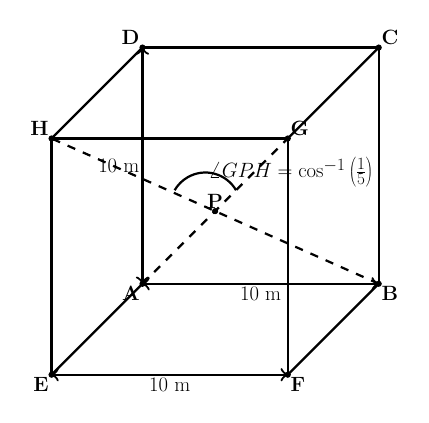
\begin{tikzpicture}[scale=0.3,transform shape]
    \coordinate (A) at (0, 0, 0);
    \coordinate (B) at (10, 0, 0);
    \coordinate (C) at (10, 10, 0);
    \coordinate (D) at (0, 10, 0);
    \coordinate (E) at (0, 0, 10);
    \coordinate (F) at (10, 0, 10);
    \coordinate (G) at (10, 10, 10);
    \coordinate (H) at (0, 10, 10);
    
    \coordinate (P) at (5, 5, 5); 

    \draw[thick] (A) -- (B) -- (C) -- (D) -- cycle;
    \draw[thick] (E) -- (F) -- (G) -- (H) -- cycle; 
    \draw[thick] (A) -- (E);
    \draw[thick] (B) -- (F);
    \draw[thick] (C) -- (G);
    \draw[thick] (D) -- (H);
    
    \draw[dashed, thick] (A) -- (G);
    \draw[dashed, thick] (B) -- (H);

    \foreach \point in {A, B, C, D, E, F, G, H, P} {
        \filldraw[black] (\point) circle (3pt);
    }

    \node at (A) [below left] {\Huge \textbf{A}};
    \node at (B) [below right] {\Huge \textbf{B}};
    \node at (C) [above right] {\Huge \textbf{C}};
    \node at (D) [above left] {\Huge \textbf{D}};
    \node at (E) [below left] {\Huge \textbf{E}};
    \node at (F) [below right] {\Huge \textbf{F}};
    \node at (G) [above right] {\Huge \textbf{G}};
    \node at (H) [above left] {\Huge \textbf{H}};
    \node at (P) [above] {\Huge \textbf{P}};

    \draw[<->, thick] (A) -- (B) node[midway, below] {\Huge 10 m};
    \draw[<->, thick] (A) -- (D) node[midway, left] {\Huge 10 m};
    \draw[<->, thick] (E) -- (F) node[midway, below] {\Huge 10 m};

    \draw[thick] (5.5, 5.5, 4) arc[start angle=30, end angle=150, radius=1.5] node[midway, right] {\Huge $\angle GPH = \cos^{-1}\left(\frac{1}{5}\right)$};

\end{tikzpicture}


\end{center}    
\begin{multicols}{4}
\begin{enumerate}
    \item $5$
    \item $2\sqrt{10}$
    \item $5\sqrt{3}$
    \item $5\sqrt{2}$
\end{enumerate}
\end{multicols}


%\end{enumerate}
%\end{document}




\iffalse
    \title{2021}
    \author{AI24BTECH11030}
    \section{mcq-single}
\fi

    \item Let $f : \mathbb{R} \rightarrow \mathbb{R}$ be a continuous function. Then
    $\lim_{x \to \frac{\pi}{4}} \frac{\frac{\pi}{4} \int_{2}^{\sec^2 x} f(x) dx}{ x^2 - \frac{\pi^2}{16}}$
    is equal to: \hfill [Aug 2021]
    \begin{multicols}{4}
        \begin{enumerate}
            \item $f(2)$
            \item $2f(2)$
            \item $2f(\sqrt{2})$
            \item $4f(2)$
        \end{enumerate}
    \end{multicols}
    
    \item $\cos^{-1}(\cos(-5)) + \sin^{-1}(\sin(6)) - \tan^{-1}(\tan(12))$ is equal to: \hfill [Aug 2021]
    \begin{multicols}{4}
        \begin{enumerate}
            \item $3\pi - 11$
            \item $4\pi - 9$
            \item $4\pi - 11$
            \item $3\pi + 1$
        \end{enumerate}
    \end{multicols}

    \item Consider the system of linear equations:
    \begin{align*}
        -x + y + 2z &= 0 \\
        3x - ay + 5z &= 1 \\
        2x - 2y - az &= 7
    \end{align*}
    Let $S_1$ be the set of all $a \in \mathbb{R}$ for which the system is inconsistent, and $S_2$ the set of all $a \in \mathbb{R}$ for which the system has infinitely many solutions. If $n(S_1)$ and $n(S_2)$ denote the number of elements in $S_1$ and $S_2$ respectively, then: \hfill [Aug 2021]
    \begin{multicols}{2}
        \begin{enumerate}
            \item $n(S_1) = 2$, $n(S_2) = 2$
            \item $n(S_1) = 1$, $n(S_2) = 0$
            \item $n(S_1) = 2$, $n(S_2) = 0$
            \item $n(S_1) = 0$, $n(S_2) = 2$
        \end{enumerate}
    \end{multicols}
    
    \item Let the acute angle bisector of the planes $x - 2y - 2z + 1 = 0$ and $2x - 3y - 6z + 1 = 0$ be the plane $P$. Which of the following points lies on $P$? \hfill [Aug 2021]
    \begin{multicols}{2}
        \begin{enumerate}
            \item $(3, 1, -\frac{1}{2})$
            \item $(-2, 0, -\frac{1}{2})$
            \item $(0, 2, -4)$
            \item $(4, 0, -2)$
        \end{enumerate}
    \end{multicols}

    \item Which of the following is equivalent to the Boolean expression $p \land \neg q$? \hfill [Aug 2021]
    \begin{multicols}{4}
        \begin{enumerate}
            \item $\neg(q \to p)$
            \item $\neg p \to \neg q$
            \item $\neg(p \to \neg q)$
            \item $\neg(p \to q)$
        \end{enumerate}
    \end{multicols}
    
    \item Two squares are chosen at random on a chessboard. The probability that they have a side in common is: \hfill [Aug 2021]
    \begin{multicols}{4}
        \begin{enumerate}
            \item $\frac{2}{7}$
            \item $\frac{1}{18}$
            \item $\frac{1}{7}$
            \item $\frac{1}{9}$
        \end{enumerate}
    \end{multicols}

    \item If $y = y(x)$ is the solution of the differential equation $x^2 dy + \brak{y - \frac{1}{x}} dx = 0$; $x > 0$ and $y(1) = 1$, then $y\brak{\frac{1}{2}}$ is equal to: \hfill [Aug 2021]
    \begin{multicols}{4}
        \begin{enumerate}
            \item $\frac{3}{2} - \frac{1}{\sqrt{e}}$
            \item $3 + \frac{1}{\sqrt{e}}$
            \item $3 + e$
            \item $3 - e$
        \end{enumerate}
    \end{multicols}

    \item If $n$ is the number of solutions of the equation
    $$
    2\cos x\brak{4\sin\brak{\frac{\pi}{4} + x} \sin\brak{\frac{\pi}{4} - x} -1 } = 1, \: x \in [0, \pi],
    $$
    and $S$ is the sum of all these solutions, then the ordered pair $(n, S)$ is: \hfill [Aug 2021]
    \begin{multicols}{4}
        \begin{enumerate}
            \item $(3, \frac{13\pi}{9})$
            \item $(2, \frac{2\pi}{3})$
            \item $(2, \frac{8\pi}{9})$
            \item $(3, \frac{5\pi}{3})$
        \end{enumerate}
    \end{multicols}

    \item The function $f(x) = x^3 - 6x^2 + ax + b$ is such that $f(2) = f(4) = 0$. Consider two statements:
    \begin{itemize}
        \item[(S1)] There exists $x_1, x_2 \in (2, 4)$, $x_1 < x_2$, such that $f'(x_1) = -1$ and $f'(x_2) = 0$.
        \item[(S2)] There exists $x_3, x_4 \in (2, 4)$, $x_3 < x_4$, such that $f$ is decreasing in $(2, x_4)$, increasing in $(x_4, 4)$ and $2f'(x_3) = \sqrt{3}f(x_4)$.
    \end{itemize}
    Then:  \hfill [Aug 2021]
    \begin{multicols}{2}
        \begin{enumerate}
            \item Both (S1) and (S2) are true
            \item (S1) is false and (S2) is true
            \item Both (S1) and (S2) are false
            \item (S1) is true and (S2) is false
        \end{enumerate}
    \end{multicols}

    \item Let 
    $$
    J_{n,m} = \int_0^\frac{1}{2} \frac{x^n}{x^m-1} dx, \forall n > m \quad \text{and} \quad n, m \in \mathbb{N}.
    $$
    Consider a matrix $A = [a_{ij}]_{3 \times 3}$ where 
    $$
    a_{ij} = \begin{cases} 
    J_{6+i,3} - J_{i+3,3}, & \text{if } i \leq j, \\
    0, & \text{if } i > j.
    \end{cases}
    $$
    Then $\abs{\text{adj} A^{-1}}$ is: \hfill [Aug 2021]
    \begin{multicols}{4}
        \begin{enumerate}
            \item $(15)^2 \times 2^{42}$
            \item $(15)^2 \times 2^{34}$
            \item $(105)^2 \times 2^{38}$
            \item $(105)^2 \times 2^{36}$
        \end{enumerate}
    \end{multicols}

    \item The area enclosed by the curves $y = \abs{\cos x - \sin x}$ and $y = \sin x + \cos x$, and the lines $x = 0$ and $x = \frac{\pi}{2}$ is: \hfill [Aug 2021]
    \begin{multicols}{4}
        \begin{enumerate}
            \item $2\sqrt{2} - 2$
            \item $2 + 2\sqrt{2}$
            \item $4 - 2\sqrt{2}$
            \item $2 + 4\sqrt{2}$
        \end{enumerate}
    \end{multicols}

    \item The distance of the line $3y - 2z - 1 = 0 = 3x - z + 4$ from the point $(2, -1, 6)$ is: \hfill [Aug 2021]
    \begin{multicols}{4}
        \begin{enumerate}
            \item $\sqrt{26}$
            \item $2\sqrt{5}$
            \item $2\sqrt{6}$
            \item $4\sqrt{2}$
        \end{enumerate}
    \end{multicols}

    \item Consider the parabola with vertex $\brak{\frac{1}{2}, \frac{3}{4}}$ and the directrix $y = \frac{1}{2}$. Let $P$ be the point where the parabola meets the line $x = -\frac{1}{2}$. If the normal to the parabola at $P$ intersects the parabola again at the point $Q$, then $(PQ)^2$ is equal to: \hfill [Aug 2021]
    \begin{multicols}{4}
        \begin{enumerate}
            \item $\frac{75}{8}$
            \item $\frac{125}{16}$
            \item $\frac{25}{2}$
            \item $\frac{15}{2}$
        \end{enumerate}
    \end{multicols}

    \item The number of pairs $(a, b)$ of real numbers, such that whenever $\alpha$ is a root of the equation $x^2 + ax + b = 0$, $\alpha^2 - 2$ is also a root of the equation, is: \hfill [Aug 2021]
    \begin{multicols}{4}
        \begin{enumerate}
            \item 6
            \item 2
            \item 4
            \item 8
        \end{enumerate}
    \end{multicols}

    \item Let $S_n = 1\cdot(n-1) + 2\cdot(n-2) + \dots + (n-1)\cdot1$, for $n \geq 4$. The sum 
    $$
    \sum_{n=4}^{\infty} \brak{\frac{2S_n}{n!} - \frac{1}{(n-2)!}}
    $$
    is equal to: \hfill [Aug 2021]
    \begin{multicols}{4}
        \begin{enumerate}
            \item $\frac{e - 1}{3}$
            \item $\frac{e - 2}{6}$
            \item $\frac{e}{3}$
            \item $\frac{e}{6}$
        \end{enumerate}
    \end{multicols}


\iffalse
    \title{2021}
    \author{EE24BTECH11001}
    \section{mcq-single}
\fi
\item 
        Let $P_1, P_2 \dots P_{15}$  be 15 points on a circle. The number of distinct triangles formed by points $P_i, P_j, P_k$ such that 
        $i + j +k \ne 0$ is :
        \hfill{\brak{\textnormal{2021-Sep}}}
        \begin{multicols}{4}
            \begin{enumerate}
                \item 12
                    \columnbreak
                \item 419
                    \columnbreak
                \item 443
                    \columnbreak
                \item 455
            \end{enumerate}
        \end{multicols}

    \item The range of the function 
        \begin{align}
            f\brak{x} = \log_{\sqrt{3}} \brak{3 + \cos \brak{\frac{3\pi}{4} + x} + \cos \brak{\frac{\pi}{4} + x}+ \cos \brak{\frac{\pi}{4} - x} +\cos \brak{\frac{3\pi}{4} - x}}
        \end{align} is :
        \hfill{\brak{\textnormal{2021-Sep}}}
        \begin{multicols}{4}
            \begin{enumerate}
                \item $\brak{0,  \sqrt{5}}$ \columnbreak
                \item $\sbrak{-2, 2}$ \columnbreak
                \item $\sbrak{\frac{1}{\sqrt{5}}, \sqrt{5}}$ \columnbreak
                \item $\sbrak{0, 2}$
            \end{enumerate}
        \end{multicols}


    \item Let $a_1, a_2 \dots a_{21}$ be an AP such that 
        \begin{align}
            \sum_{n = 1} ^{20} \frac{1}{a_{n}a_{n+1}} = \frac{4}{9}
        \end{align}. If the sum of the AP is 189, then $a_{6}a_{16}$ is : 
        \hfill{\brak{\textnormal{2021-Sep}}}
        \begin{enumerate}
                \begin{multicols}{2}
                \item 57 \columnbreak
                \item 72
                \end{multicols}
                \begin{multicols}{2}
                \item 48 \columnbreak
                \item 36
                \end{multicols}
        \end{enumerate}

    \item  The function $f\brak{x}$, that satisfies the condition  
        \begin{align}
            f\brak{x} = x + \int_{0} ^ {\frac{\pi}{2}} \sin x \cos y f\brak{y} \, dy
        \end{align} 
        is : 
        \hfill{\brak{\textnormal{2021-Sep}}}
        \begin{enumerate}
                \begin{multicols}{4}
                \item $x + \frac{2}{3}\brak{\pi - 2}\sin x$ \columnbreak
                \item $x + \brak{\pi + 2}\sin x$ \columnbreak
                \item $x + \frac{\pi}{2}\sin x$ \columnbreak
                \item $x + \brak{\pi - 2}\sin x$
                \end{multicols}
        \end{enumerate}

    \item Let $\theta$ be the acute angle between the tangents to the ellipse 
        \begin{align}
            \frac{x^2}{9} + \frac{y^2}{1} = 1
        \end{align} and the circle 
        \begin{align}
            x^2 + y^2 = 3
        \end{align} at their point of intersection in the first quadrant. Then $\tan \theta$ is equal to :

        \hfill{\brak{\textnormal{2021-Sep}}}
        \begin{enumerate}
            \item $\frac{5}{2\sqrt{2}}$ 
            \item $\frac{2}{\sqrt{3}}$ 
            \item $\frac{4}{\sqrt{3}}$  
            \item $2$
        \end{enumerate}

\iffalse
  \title{Assignment}
  \author{EE24BTECH11038}
  \section{mcq-single}
\fi  
\item Let $p_1,p_2,p_3,\cdots,p_{15}$ be points on circle. The number of distinct triangles formed by points $p_i,p_j,p_k$ such that i+j+k$\neq$15, is :\hfill{Aug 2021}
\begin{enumerate}
    \item 12
    \item 419
    \item 443
    \item 455
\end{enumerate}
\bigskip
\item The range of the function,
\begin{align*}
    f\brak{x}=\log_{\sqrt{5}} \left(3+\cos{\brak{\frac{3\pi}{4}+x}}+\cos{\brak{\frac{\pi}{4}+x}}+\cos{\brak{\frac{\pi}{4}-x}}-\cos{\brak{\frac{3\pi}{4}-x}}\right)
\end{align*}
is:\hfill{Aug 2021}
\begin{enumerate}
    \item $\brak{0,\sqrt{5}}$\\
    \item $\sbrak{-2,2}$\\
    \item $\sbrak{\frac{1}{\sqrt{5}},\sqrt{5}}$\\
    \item $\sbrak{0,2}$
\end{enumerate}
\bigskip
\item Let $a_1,a_2,a_3,\cdots,a_{21}$ be an A.P such that $\sum_{n=1}^{20} \frac{1}{a_na_{n+1}}=\frac{4}{9}$. If the sum of this A.P is 189, then $a_6a_{16}$ is equal to :\hfill{Aug 2021}
\begin{enumerate}
    \item 57
    \item 72
    \item 48
    \item 36
\end{enumerate}
\bigskip
\item The function f$\brak{x}$, that satisfies the condition f$\brak{x}$=x+$\int_0^{\frac{\pi}{2}} \sin{x}.\cos{y}f\brak{y}\,dy,$ is :\hfill{Aug 2021}
\begin{enumerate}
    \item x+$\frac{2}{3}\brak{\pi-2}\sin{x}$
    \item  x+$\brak{\pi+2}\sin{x}$
     \item x+$\frac{\pi}{2}\sin{x}$
      \item x+$\brak{\pi-2}\sin{x}$
\end{enumerate}
\bigskip
\item Let $\theta$ be the acute angle between the tangents to the ellipse $\frac{x^2}{9}+\frac{y^2}{1}$=1 and the circle $x^2+y^2=3$ at their point of intersection in the first quadrant then $\tan{\theta}$ is equal to:\hfill{Aug 2021}
\begin{enumerate}
    \item $\frac{5}{2\sqrt{3}}$
    \item $\frac{2}{\sqrt{3}}$
    \item $\frac{4}{\sqrt{3}}$
    \item 2
\end{enumerate}



\iffalse
\title{2021}
\author{EE24BTECH11012}
\section{mcq-single}
\fi

%\begin{enumerate}
	\item Let $\vec{A}$ and $\vec{B}$ be $3 \times 3$ real matrices such that $\vec{A}$ is symmetric matrix and $\vec{B}$ is skew-symmetric matrix. Then the sytem of linear equations $\brak{\vec{A^2B^2 - B^2A^2}}\vec{X} = \vec{O}$, where $\vec{X}$ is a $3 \times 1$ column matrix of unknown variables and $\vec{O}$ is a $3 \times 1$ null matrix, has: \hfill{[Feb 2021]} 
		\begin{enumerate}
			\item a unique solution
			\item exactly two solutions
			\item infinitely many solutions
			\item no solution
		\end{enumerate}
	\item If $ n\geq2 $ is a positive integer, then the sum of the series $\comb{n+1}{2} + 2\brak{\comb{2}{2} + \comb{3}{2} + \comb{4}{2} + \dots + \comb{n}{2}}$ is \hfill{[Feb 2021]}
		\begin{enumerate}
				\begin{multicols}{4}
				\item $ \frac{n\brak{n+1}^2\brak{n+2}}{12}$
				\item $ \frac{n\brak{n-1}\brak{2n+1}}{6} $
				\item $ \frac{n\brak{n+1}\brak{2n+1}}{6} $
				\item $ \frac{n\brak{2n+1}\brak{3n+1}}{6} $
				\end{multicols}
		\end{enumerate}
	\item If a curve $ y = f\brak{x} $ passes through the point $\myvec{1,2}$ and satisfies $ x\frac{dy}{dx} + y = \emph{b}x^4 $, then for what value of \emph{b}, $ \int_{1}^{2} f\brak{x} dx = \frac{62}{5} $ holds good ?\hfill{[Feb 2021]}
		\begin{enumerate}
				\begin{multicols}{4}
			\item 5
			\item $\frac{62}{5}$
			\item $\frac{31}{5}$
			\item 10
				\end{multicols}
		\end{enumerate}
	\item The area of the region: $ \textbf{R}\cbrak{\myvec{x,y} : 5x^2 \leq y \leq 2x^2 + 9 } $ is :\hfill{[Feb 2021]}
		\begin{enumerate}
				\begin{multicols}{4}
				\item $ 9\sqrt3 $
				\item $ 12\sqrt3 $
				\item $ 11\sqrt3 $
				\item $ 6\sqrt3 $
				\end{multicols}
		\end{enumerate}
	\item Let f\brak{x} be a differentiable function defined on \sbrak{0,2} such that $ f^{\prime}\brak{x} = f^{\prime}\brak{2-x} $ for all x $\in$ \brak{0,2}, $ f\brak{0} = 1 $ and $ f\brak{2} = e^2 $ . Then the value of $ \int_{0}^{2} f\brak{x} dx $ is: \hfill{[Feb 2021]}
		\begin{enumerate}
				\begin{multicols}{4}
				\item $ 1+e^2 $
				\item $ 1-e^2 $
				\item $ 2\brak{1-e^2} $
				\item $ 2\brak{1+e^2} $
				\end{multicols}
		\end{enumerate}
%\end{enumerate}

\iffalse
\title{Assignment}
\author{ee24btech11059}
\section{mcq-single}
\fi

    \item{
          	A plane passes through the points $A\brak{1,2,3}$, $B\brak{2,3,1}$ and $C\brak{2,4,2}$. If $O$ is the origin and $P$ is $\brak{2,-1,1}$, then the projection of vector $\overrightarrow{OP}$ on this plane is of length:\\ \text{  }\hfill
                {[Feb 2021]}
            \begin{multicols}{4}
				\begin{enumerate}
					\item $\sqrt{\frac{2}{5}}$
					
					\item $\sqrt{\frac{2}{3}}$
					
					\item $\sqrt{\frac{2}{11}}$
					
					\item $\sqrt{\frac{2}{7}}$
				\end{enumerate}
			\end{multicols}
            }
    %code by ysiddhanth 
    \item{
           	The contrapositive of the statement “If you will work, you will earn money” is: \\ \text{ }\hfill
                {[Feb 2021]}
                \begin{enumerate}
                   	\item If you will not earn money, you will not work
                   	\item You will earn money, if you will not work
                   	\item If you will earn money, you will work
                   	\item To earn money, you need to work
                \end{enumerate}
        }
\item{
        	
        	If $\alpha, \beta \in \mathbb{R}$ are such that $1 - 2i$ (here $i^2 = -1$) is a root of $z^2 + \alpha z + \beta = 0$, then $\brak{\alpha - \beta}$ is equal to:
        	\hfill
        	{[Feb 2021]}
        	\begin{multicols}{4}
        		\begin{enumerate}
        			\item 7
        			\item -3
        			\item -7
        			\item 3
        		\end{enumerate}
        	\end{multicols}
        	
        }
    \item{
     
            If $\int_{\pi/4}^{\pi/2}cot^nx dx$, then:\hfill
                {[Feb 2021]}
            \begin{multicols}{2}
                \begin{enumerate}
                    \item $\frac{1}{I_2 + I_4}$, $\frac{1}{I_3 + I_5}$, $\frac{1}{I_4 + I_6}$ are in G.P.
                    
                    \item $\frac{1}{I_2 + I_4}$, $\frac{1}{I_3 + I_5}$, $\frac{1}{I_4 + I_6}$ are in A.P.
                    
                    \item $I_2 + I_4$, $I_3 + I_5$, $I_4 + I_6$ are in A.P.
                    
                    \item $I_2 + I_4$, $I_3 + I_5$, $I_4 + I_6$ are in G.P.
                \end{enumerate}
            \end{multicols}
        
        }
    \item{
            $A = \myvec{ 1 & -\alpha \\ \alpha & \beta}$, $ AA^\top = I_2, \text{ then the value of } \alpha^4 + \beta^4 \text{ is:} $
           	\hfill
                {[Feb 2021]}
            
            \begin{multicols}{4}
				\begin{enumerate}
					\item 1
					\item 2
					\item 3
					\item 4
				\end{enumerate}
			\end{multicols}
        
        }
 	\item{
        	Let $x$ denote the total number of one-one functions from a set $A$ with 3 elements to a set $B$ with 5 elements and $y$ denote the total number of one-one functions from the set $A$ to the set $A \times B$. Then:\\ \text{ }
        	\hfill
        	{[Feb 2021]}
        	
        	\begin{multicols}{4}
        		\begin{enumerate}
					\item $y = 273x$
					
					\item $2y = 91x$
					
					\item $y = 91x$
					
					\item $2y = 273x$
        		\end{enumerate}
        	\end{multicols}
        	
        }
 	\item{
			If the curve $x^2 + 2y^2 = 2$ intersects the line $x + y = 1$ at two points P and Q, then the angle subtended by the line segment PQ at the origin is:
			\hfill
			{[Feb 2021]}
			
			\begin{multicols}{4}
				\begin{enumerate}
					\item $\frac{\pi}{2} + \tan^{-1}\brak{\frac{1}{4}}$
					\item $\frac{\pi}{2} - \tan^{-1}\brak{\frac{1}{4}}$
					\item $\frac{\pi}{2} + \tan^{-1}\brak{\frac{1}{3}}$
					\item $\frac{\pi}{2} - \tan^{-1}\brak{\frac{1}{3}}$
				\end{enumerate}
			\end{multicols}
			
		}
 	\item{
			The integral $\int\frac{e^{3log_{e}2x} + 5e^{2log_{e}2x}}{e^{4log_{e}x}+ 5e^{3log_{e}x} - 7e^{2log_{e}x}}, x>0$ is equal to:\\ \text{ }
			\hfill
			{[Feb 2021]}
			
			\begin{multicols}{2}
				\begin{enumerate}
					\item $\log_e |x^2 + 5x - 7| + c$
					
					\item $\frac{1}{4} \log_e |x^2 + 5x - 7| + c$
					
					\item $4 \log_e |x^2 + 5x - 7| + c$
					
					\item $\log_e \sqrt{x^2 + 5x - 7} + c$
				\end{enumerate}
			\end{multicols}
			
		}
    \item{
            A hyperbola passes through the foci of the ellipse $\frac{x^2}{25} + \frac{y^2}{16} = 1$ and its transverse and conjugate axes coincide with major and minor axes of the ellipse, respectively. If the product of their eccentricities is one, then the equation of the hyperbola is:\\ \text{ }
             \hfill
                {[Feb 2021]}
            \begin{multicols}{2}
                \begin{enumerate}
                    \item $\frac{x^2}{9} - \frac{y^2}{4} = 1$
                    
                    \item $\frac{x^2}{9} - \frac{y^2}{16} = 1$
                    
                    \item $x^2 - y^2 = 9$
                    
                    \item $\frac{x^2}{9} - \frac{y^2}{25} = 1$
                \end{enumerate}
            \end{multicols}

        %code by ysiddhanth 
        
        }
    \item{
            $\lim_{n \rightarrow \infty}\sbrak{\frac{1}{n} + \frac{n}{\brak{n+1}^2} + \frac{n}{\brak{n+2}^2} +……+ \frac{n}{\brak{2n-1}^2}}$ is equal to: 
             \hfill
                {[Feb 2021]}
            \begin{multicols}{4}
                \begin{enumerate}
                	\item 1
                	\item $\frac{1}{3}$
                	\item $\frac{1}{2}$
                	\item $\frac{1}{4}$
                \end{enumerate}
            \end{multicols}
        
        }
    \item{
            In a group of 400 people, 160 are smokers and non-vegetarian; 100 are smokers and vegetarian and the remaining 140 are non-smokers and vegetarian. Their chances of getting a particular chest disorder are 35\%, 20\% and 10\% respectively. A person is chosen from the group at random and is found to be suffering from chest disorder. The probability that the selected person is a smoker and non-vegetarian is: \\ \text{ }
             \hfill
                {[Feb 2021]}
			\begin{multicols}{4}
				\begin{enumerate}
					\item $\frac{7}{45}$  
					\item $\frac{8}{45}$  
					\item $\frac{14}{45}$  
					\item $\frac{28}{45}$
				\end{enumerate}
			\end{multicols}
        
        }
    \item{
        	The following system of equations,
            $
            	2x + 3y + 2z = 9 ,
            	3x + 2y + 2z = 9 ,
            	x - y + 4z = 8
            $
             \text{   }\hfill
                {[Feb 2021]}

                \begin{enumerate}
                   	\item does not have any solution 
                   	\item has a unique solution 
                   	\item has a solution $\brak{\alpha, \beta, \gamma}$ satisfying $\alpha + \beta^2 + \gamma^3 = 12$ 
                   	\item has infinitely many solutions
                \end{enumerate}

        
        }
    \item{
	
			The minimum value of
			$ f\brak{x} = a^{a^{x}} + a^{1-a^{x}}$
			where $a, x \in \mathbb{R}$ and $a > 0$, is equal to:\\
			\text{   }\hfill
			{[Feb 2021]}
			\begin{multicols}{4}
				\begin{enumerate}
						\item $a + \frac{1}{a}$
						\item $a + 1$
						\item $2a$
						\item $2\sqrt{a}$
				\end{enumerate}
			\end{multicols}
			
		}
    \item{
	
			The function \( f\brak{x} \) is given by \( f\brak{x} = \frac{5x}{5x+5} \), then the sum of the series \( f\brak{\frac{1}{20}} + f\brak{\frac{2}{20}} + f\brak{\frac{3}{20}} + \ldots + f\brak{\frac{39}{20}} \) is equal to:
			\text{   }\hfill
			{[Feb 2021]}
			\begin{multicols}{4}
				\begin{enumerate}
					\item $\frac{19}{2}$
					\item $\frac{49}{2}$
					\item $\frac{39}{2}$
					\item $\frac{29}{2}$
				\end{enumerate}
			\end{multicols}
			
		}
    \item{
        
            Let $\alpha$ and $\beta$ be the roots of $x^2 - 6x - 2 = 0$. If $a_n = \alpha^n - \beta^n$ for $n \geq 1$, then the value of $\frac{a_{10} - 2a_8}{3a_9}$ is:
             \hfill
              {[Feb 2021]}
              \begin{multicols}{4}
	              	\begin{enumerate}
	              		\item 4
	              		\item 1
	              		\item 2
	              		\item 3
	              	\end{enumerate}
              \end{multicols}
        
        }



\iffalse
\title{2021}
\author{AI24BTECH11031}
\section{mcq-single}
\fi

\item The value of $\lim\limits_{h \to 0} 2\cbrak{\frac{\sqrt{3}\sin\brak{\frac{\pi}{6} - h} - \cos\brak{\frac{\pi}{6} + h}}{\sqrt{3}h\brak{\sqrt{3}\cos h - \sin h}}}$ is
\hfill{[Feb 2021]}

\begin{multicols}{4}
\begin{enumerate}
    \item $\frac{3}{4}$
    \item $\frac{2}{\sqrt{3}}$
    \item $\frac{4}{3}$
    \item $\frac{2}{3}$
\end{enumerate}
\end{multicols}

\item A fair coin is tossed a fixed number of times. If the probability of
getting 7 heads is equal to the probability of getting 9 heads, then the
probability of getting 2 heads is:
\hfill{[Feb 2021]}

\begin{multicols}{4}
\begin{enumerate}
    \item $\frac{15}{2^{12}}$
    \item $\frac{15}{2^{13}}$
    \item $\frac{15}{2^{14}}$
    \item $\frac{15}{2^{8}}$
\end{enumerate}
\end{multicols}

\item If $(1, 5, 35)$, $(7, 5, 5)$, $(1, \lambda, 7)$ and $(2\lambda, 1, 2)$ are
coplanar, then the sum of all possible values of $\lambda$ is:
\hfill{[Feb 2021]}

\begin{multicols}{4}
\begin{enumerate}
    \item $-\frac{44}{5}$
    \item $\frac{39}{5}$
    \item $-\frac{39}{5}$
    \item $\frac{44}{5}$
\end{enumerate}
\end{multicols}

\item Let $R = \cbrak{(P,Q) \mid \text{P and Q are at the same distance from the origin}}$
be a relation, then the equivalence class of $(1,-1)$ is the set:
\hfill{[Feb 2021]}

\begin{multicols}{2}
\begin{enumerate}
    \item $S = \cbrak{(x, y) \mid x^2 + y^2 = 1}$
    \item $S = \cbrak{(x, y) \mid x^2 + y^2 = 4}$
    \item $S = \cbrak{(x, y) \mid x^2 + y^2 = \sqrt{2}}$
    \item $S = \cbrak{(x, y) \mid x^2 + y^2 = 2}$
\end{enumerate}
\end{multicols}

\item In the circle given below, let $OA$ = 1 unit,
$OB$ = 13 unit and $PQ$ perpendicular to $OB$. Then, the area
of the triangle $PQB$ (in square units) is:
\hfill{[Feb 2021]}

\begin{center}
\begin{tikzpicture}
    \draw [->] (0, -2) -- (0, 2) node[left] {Y};
    \draw [->] (-2, 0) -- (4, 0) node[right] {X};
    \draw (1, 0) circle (1);
    \draw (2, 0) node[below right] {B} --
            (0.5, -0.86) node[below] {Q} --
            (0.5, 0.86) node[above] {P} -- (2, 0);
    \draw (0, 0) node[below left] {O} -- (0.5, 0) node[below right] {A};
\end{tikzpicture}
\end{center}

\begin{multicols}{4}
\begin{enumerate}
    \item $26 \sqrt{3}$
    \item $24 \sqrt{2}$
    \item $24 \sqrt{3}$
    \item $26 \sqrt{2}$
\end{enumerate}
\end{multicols}

\iffalse
    \title{2021}
    \author{EE24BTECH11001}
    \section{mcq-single}
\fi
\item 
		The number of seven-digit integers with the sum of the digits equal to 10 and formed by using the digits 1, 2 and 3 only is :
		\hfill{\brak{2021-Feb}}
	\begin{multicols}{4}
		\begin{enumerate}
			\item 77 
			\columnbreak
			\item 42
			\columnbreak
			\item 35
			\columnbreak
			\item 82
		\end{enumerate}
	\end{multicols}

	\item
		The maximum value of the term independent of $'t'$ in the expression of
		$\sbrak{\brak{tx^{\frac{1}{5}}+ \{ \frac{1 - x}{t}\}} ^{\frac{1}{10}}}^{10}$ where
		$x \in \brak{0, 1}$ is :
		\hfill{\brak{2021-Feb}}
		\begin{multicols}{4}
		\begin{enumerate}
			\item $\frac{10!}{\sqrt{3}\brak{5!}^{2}}$ \columnbreak
			\item $\frac{2 . 10!}{3\brak{5!}^2}$ \columnbreak
			\item $\frac{10!}{3\brak{5!}^2}$ \columnbreak
			\item $\frac{2 . 10!}{3\sqrt{3}\brak{5!}^2}$
		\end{enumerate}
	\end{multicols}


\item The value of 
	\begin{align}
		\sum_{n = 1}^{100} \int_{n - 1}^n e^{x - \sbrak{x}} \, dx
	\end{align} where $\sbrak{x}$ is the greatest integer $\le x$
		\hfill{\brak{2021-Feb}}
		\begin{enumerate}
			\begin{multicols}{2}
			\item $100\brak{e - 1}$ \columnbreak
			\item $100e$
			\end{multicols}
			\begin{multicols}{2}
			\item $100\brak{1 - e}$ \columnbreak
			\item $100\brak{1 + e}$
			\end{multicols}
		\end{enumerate}
		
	\item The rate of growth of bacteria in a culture is proportional to the number of bacteria present and the bacteria cout is $1000$ at initial time $t = 0$. The number of bacteria is increased by $20\%$ in 2 hours. If the population of bacteria is $2000$ after $\frac{k}{\log_e \brak{\frac{6}{5}}}$ hours, then $\brak{\frac{k}{\log_e 2}}^2 $is equal to :
		\hfill{\brak{2021-Feb}}
		\begin{enumerate}
			\begin{multicols}{4}
				\item 1 \columnbreak
				\item 2 \columnbreak
				\item 16 \columnbreak
				\item 8
			\end{multicols}
		\end{enumerate}

	\item If $\vec{a}$ and $\vec{b}$ are perpendicular, then 
	\begin{align*}
		\vec{a} \times \left(\vec{a} \times \left(\vec{a} \times \left(\vec{a} \times \vec{b}\right)\right)\right)
	\end{align*}
	is equal to 
		\hfill{\brak{2021-Feb}}
		\begin{enumerate}
			\item $\frac{1}{2}\norm{\vec{a}}^4 \vec{b}$ 
			\item $\vec{a} \times \vec{b}$ 
			\item $\norm{\vec{a}}^4 \vec{b}$  
			\item $\vec{0}$
		\end{enumerate}
	\item
		In an increasing geometric series, the sum of the second and the sixth terms is $\frac{25}{2}$
		and the product of the third and fifth term is 25. Then, the sum of $4^{th}, 6^{th}$ and $8^{th}$ terms
		is equal to :
		\hfill{\brak{2021-Feb}}
		\begin{multicols}{4}
		\begin{enumerate}
			\item 35 \columnbreak
			\item 30 \columnbreak
			\item 26 \columnbreak
			\item 32
		\end{enumerate}
	\end{multicols}
	\item Consider the three planes
		\begin{enumerate}
			\item[P1 :] $3x + 15y + 21z = 9,$
			\item[P2 :] $x - 3y - z = 5, $and 
			\item[P3 :] $2x + 10y + 14z = 5$
		\end{enumerate}
		Then, which of the following is true ?	
		\hfill{\brak{2021-Feb}}
		\begin{enumerate}
			\item P1 and P3 are parallel. 
			\item P2 and P3 are parallel. 
			\item P1 and P2 are parallel. 
			\item P1, P2 and P3 are parallel.
		\end{enumerate}
\item
	The sum of the infinite series
	\begin{align}
		1 + \frac{2}{3} + \frac{7}{3^2} + \frac{12}{3^3} + \frac{17}{3^4} + \frac{22}{3^5} + \dots
	\end{align} is equal to :
		\hfill{\brak{2021-Feb}}
	\begin{multicols}{4}
		\begin{enumerate}
			\item $\frac{9}{4}$ \columnbreak
			\item $\frac{15}{4}$ \columnbreak
			\item $\frac{13}{4}$ \columnbreak
			\item $\frac{11}{4}$
		\end{enumerate}
	\end{multicols}
\item The value of
		\begin{align}
			\mydet{
			\brak{a+1}\brak{a+2} & a+2 & 1 \\
			\brak{a+2}\brak{a+3} & a+3 & 1 \\
			\brak{a+3}\brak{a+4} & a+4 & 1
			}
		\end{align} is :
		\hfill{\brak{2021-Feb}}
	
		\begin{enumerate}
			\item -2 
			\item $\brak{a+1}\brak{a+2}\brak{a+3}$ 
			\item 0 
			\item $\brak{a+2}\brak{a+3}\brak{a+4}$
		\end{enumerate}
\item If
		\begin{align}
			\frac{\sin ^{-1}}{a} = \frac{\cos ^{-1}}{b} = \frac{\tan ^{-1}}{c};
			0 < x < 1
		\end{align}, then the value of $\cos \brak{\frac{\pi c}{a+b}}$ is :
		\hfill{\brak{2021-Feb}}
		
		\begin{enumerate}
			\item $\frac{1 - y^2}{2y}$ \\
			\item $\frac{1 - y^2}{1 + y^2}$\\
			\item $1 - y^2$ \\
			\item $\frac{1 - y^2}{y\sqrt{y}}$
		\end{enumerate}
\item Let $A$ be a symmetric matrix of order 2 with integer entries. If the sum of the diagonal
	elements of $A^2$ is 1, then the possible number of such matrices is:
		\hfill{\brak{2021-Feb}}
		
	\begin{multicols}{4}
		\begin{enumerate}
			\item 6 \columnbreak
			\item 1 \columnbreak
			\item 4 \columnbreak
			\item 12
		\end{enumerate}
	\end{multicols}
\item The intersection of the three lines x-y = 0, x + 2y = 3 and 2x + y = 6 is a :
		\hfill{\brak{2021-Feb}}
		\begin{enumerate}
			\item Equilateral triangle 
			\item Right angled triangle  
			\item Isosceles triangle 
			\item None of the above
		\end{enumerate}
		\begin{figure}
			\centering
			\begin{tikzpicture}[scale = 2]
    				\draw[black, thick, domain=1:2, samples=100] 
					plot ({\x}, {\x}); 
    				\draw[black, thick, domain=2:3, samples=100] 
					plot ({\x}, {6 - 2 *(\x)}); 
   				\draw[black, thick, domain=1:3, samples=100] 
					plot ({\x}, {1.5 - 0.5 *(\x)}); 
					
				\node [left] at (1,1.5) {$x-y = 0$};	
				\node [left] at (2,0) {$x+2y = 3$};	
				\node [left] at (4,1) {$2x+y = 6$};	
				\fill[black] (2, 2) circle (1pt) node[above] {\tiny $\brak{2, 2}$};
				\fill[black] (3, 0) circle (1pt) node[below right] {\tiny $\brak{3, 0}$};
				\fill[black] (1, 1) circle (1pt) node[below left] {\tiny $\brak{1, 1}$};		
			\end{tikzpicture}
		\end{figure}
	\item The maximum slope of the curve $y = \frac{1}{2}x^4 -5x^2 + 18x^2 -19x$ occurs at the point:
		\hfill{\brak{2021-Feb}}
	\begin{multicols}{4}
		\begin{enumerate}
			\item $\brak{2, 9}$ \columnbreak
			\item $\brak{2, 2}$ \columnbreak
			\item $\brak{3, \frac{21}{2}}$ \columnbreak
			\item $\brak{0, 0}$
		\end{enumerate}
	\end{multicols}
\item Let $f$ be any function defined on $\vec{R}$ and let it satisfy the condition: 
	\begin{align}
		\abs{f\brak{x} - f\brak{y}} \le \abs{\brak{x - y^2}}, \forall x, y \in \vec{R}
	\end{align} 
		If $f\brak{0} = 1$, then :
		\hfill{\brak{2021-Feb}}
		\begin{enumerate}
			\item $f\brak{x} < 0, \forall x \in \vec{R}$
			\item $f\brak{x}$ can take any vaule in $\vec{R}$
			\item $f\brak{x} = 0$
			\item $f\brak{x} > 0, \forall x \in \vec{R}$
		\end{enumerate}
\item The value of
		\begin{align*}
			\int_{\frac{-\pi}{2}} ^ {\frac{\pi}{2}} \frac{\cos ^2 x}{1 + 3^x} \, dx
		\end{align*} is :
		\hfill{\brak{2021-Feb}}
	\begin{multicols}{4}
		\begin{enumerate}
			\item $2\pi$ \columnbreak
			\item $4\pi$ \columnbreak
			\item $\frac{\pi}{2}$ \columnbreak
			\item $\frac{\pi}{4}$
		\end{enumerate}
	\end{multicols}

\iffalse
\title{2021}
\author{EE24BTECH11012}
\section{mcq-single}
\fi
%\begin{enumerate}
	 	
	\item Let $ g(t) = \int_{\frac{- \pi}{2}}^{\frac{\pi}{2}} \cos{\brak{\frac{\pi}{4}t + f(x)}} dx$, where $f(x) = \log{\brak{x + \sqrt{x^2 + 1}}}$, x $\in \vec{R}$. Then which of the following is correct ? \hfill{[July 2021]}
	 \begin{enumerate}
			 \begin{multicols}{4}
			 \item $g(1) = g(0)$
			 \item $\sqrt{2}g(1) = g(0)$
			 \item $g(1) = \sqrt{2}g(0)$
			 \item $g(1) + g(0) = 0$
			 \end{multicols}
	 \end{enumerate}
 \item Let P be a variable point on the parabola $y=4x^2+1$.Then the locus of the mid-point of the point P and the foot of perpendicular drawn from the point P to the line $y=x$ is :\hfill{[July 2021]}
	 \begin{enumerate}
		 \item $\brak{3x-y}^2 + \brak{x-3y} + 2 = 0$
		 \item $2 \brak{3x-y}^2 + \brak{x-3y} + 2 = 0$
		 \item $\brak{3x-y}^2 + 2\brak{x-3y} + 2 = 0$
		 \item $2 \brak{x-3y}^2 + \brak{3x-y} + 2 = 0$
	 \end{enumerate}
\item The absolute value of $k$ $ \in \vec{R}$, for which the following system of linear equations \hfill{[July 2021]}
		\begin{align}
			3x - y + 4z &= 3 \\ 
			x + 2y - 3z &= -2 \\
			6x + 5y + kz &= -3 
		\end{align}
		has infinitely many solutions is :
	\begin{enumerate}
			\begin{multicols}{4}
			\item 3
			\item -5
			\item 5
			\item -3
			\end{multicols}
	\end{enumerate}
\item If sum of the first 21 terms of the series $ \log_{9^\frac{1}{2}}{x} + \log_{9^\frac{1}{3}}{x} + \log_{9^\frac{1}{4}}{x} + \dots $, where x > 0 is 504, then x is equal to \hfill{[July 2021]}
	\begin{enumerate}
			\begin{multicols}{4}
			\item 243
			\item 9
			\item 7
			\item 81
			\end{multicols}
	\end{enumerate}
\item In a triangle ABC, if $\abs{\vec{BC}}=3$, $\abs{\vec{CA}}=5$ and $\abs{\vec{BA}}=7$, then the projection of the vector $\vec{BA}$ on $\vec{BC}$ is equal to\hfill{[July 2021]}
	\begin{enumerate}
			\begin{multicols}{4}
			\item $\frac{19}{2}$
			\item $\frac{13}{2}$
			\item $\frac{11}{2}$
			\item $\frac{15}{2}$
			\end{multicols}
	\end{enumerate}
%\end{enumerate}
%\end{document}

\iffalse
\title{Assignment}
\author{EE24BTECH11038}
\section{mcq-single}
\fi
\item  The value of $\tan \brak{{2\tan^{-1}{\frac{3}{5}+\sin^{-1}{\frac{5}{13}}}}}$ is:\hfill(July 2021)
\begin{enumerate}
    \item $\frac{220}{21}$\\
    \item $\frac{110}{21}$\\
    \item $\frac{55}{21}$\\
    \item $\frac{20}{11}$
\end{enumerate}
\item  If sum of the first 21 terms of series $\log_{9^\frac{1}{2}}^{x}+\log_{9^\frac{1}{3}}^{x}+\log_{9^\frac{1}{4}}^{x}+ \cdots $, where $x>0$ is 504, then x is equal to\hfill(July 2021)
\begin{enumerate}
    \item 243
    \item 9
    \item 7
    \item 81
\end{enumerate}
\item Two circles pass through $\brak{-1,4}$ and their centres lie on $x^2+y^2+2x+4y = 4$. If $r_1$ and $r_2$ are maximum and minimum radii and $\frac{r_1}{r_2}$ = a+$\sqrt{2}$b, then the value of a+b is\hfill(July 2021)
\begin{enumerate}
    \item 3
    \item 11
    \item 5
    \item 7
\end{enumerate}
\item If $\triangle ABC$ is a right-angled triangle with sides a,b and c and smallest angle $\theta$. If $\frac{1}{a} , \,\frac{1}{b}\, and \frac{1}{c}$ are also the sides of the right-angle triangle then find $\sin{\theta}$.\hfill(July 2021)
\begin{enumerate}
    \item $\sqrt{\frac{\brak{3-\sqrt{5}}}{2}}$\\
    \item $\frac{\brak{3-\sqrt{5}}}{2}$\\
    \item $\sqrt{\frac{\brak{3+\sqrt{5}}}{2}}$\\
    \item ${\frac{\brak{3+\sqrt{5}}}{2}}$
\end{enumerate}
\item For the natural numbers m,n if $\brak{1-y}^m\brak{1+y}^n$=1+$a_1y+a_2y^2+a_3y^3+\cdots a_{m+n}y^{m+n}$ and $a_1=a_2=10,$ then the value of $\brak{m+n}$ is equal to\hfill(July 2021)
\begin{enumerate}
    \item 88
    \item 64
    \item 100
    \item 80
\end{enumerate}



   \iffalse
   \title{Assignment}
   \author{ee24btech11059}
   \section{mcq-single}
   \fi
    \item{
          	Let $L$ be the line of intersection of planes $r \cdot \brak{i - j + 2k} = 2$ and $r \cdot \brak{2i + j - k} = 2$. If $P\brak{\alpha, \beta, \gamma}$ is the foot of perpendicular on $L$ from the point $\brak{1, 2, 0}$, then the value of $35\brak{\alpha + \beta + \gamma}$ is equal to \text{  }\hfill
                {[Jul 2021]}
                \begin{multicols}{4}
					\begin{enumerate}
						\item 101
						\item 119
						\item 143
						\item 134
					\end{enumerate}
				\end{multicols}
            }
    %code by ysiddhanth 
    \item{
           	Let $S_n$ denote the sum of the first n terms of an arithmetic progression. If $S_{10} = 530$, $S_5 = 140$, then 
           	$S_{20} - S_6$ is equal to:
           	\hfill
           	{[Jul 2021]}
                \begin{multicols}{4}
                	\begin{enumerate}
                		\item 1862
                		\item 1842
                		\item 1852
                		\item 1872
                	\end{enumerate}
                \end{multicols}
        }
\item{
        	
        	Let $f : \mathbb{R} \rightarrow \mathbb{R}$ be defined as
        	
        	\[ f\brak{x} = \begin{cases} 
        		-\frac{4}{3}x^3 + 2x^2 + 3 & \text{if } x > 0 \\
        		3xe^x & \text{if } x \leq 0 
        	\end{cases} \]
        	
        	Then $f$ is an increasing function in the interval.
        	\hfill
        	{[Jul 2021]}
        	\begin{multicols}{4}
        		\begin{enumerate}
        			\item $\brak{-\frac{1}{2}, 2}$
        			\item $\brak{0,2}$
        			\item $\brak{-1,\frac{3}{2}}$
        			\item $\brak{-3,-1}$
        		\end{enumerate}
        	\end{multicols}
        	
        }
    \item{
     
            Let $y=y\brak{x}$ be the solution of the differential equation $\csc^2x dy + 2dx = \brak{1+y \cos 2x} \csc^2x dx$, with $y\brak{\pi/4} = 0$. Then, the value of $\brak{y(0)+1}^2$ is equal to: \\ \text{ }
            \hfill
            {[Jul 2021]}
            \begin{multicols}{4}
                \begin{enumerate}
                	\item $e^\frac{1}{2}$
                	\item $e^{-\frac{1}{2}}$
                	\item $e^{-1}$
                	\item $e$
                \end{enumerate}
            \end{multicols}
        
        }
    \item{
            Four dice are thrown simultaneously and the numbers shown on these dice are recorded in $2\times 2$
            matrices. The probability that such formed matrices have all different entries and are non-singular, is :
           	\hfill
                {[Jul 2021]}
            
            \begin{multicols}{4}
				\begin{enumerate}
					\item $\frac{45}{162}$
					\item $\frac{23}{81}$
					\item $\frac{22}{81}$
					\item $\frac{43}{162}$
				\end{enumerate}
			\end{multicols}
        
        }
 	\item{
        	Let a vector $\overrightarrow{a}$ be coplanar with vectors $\overrightarrow{b} = 2\hat{i} + \hat{j}  + \hat{k} $ and $\overrightarrow{c} = \hat{i}  - \hat{j}  + \hat{k} $. If $\overrightarrow{a}$ is perpendicular to $\overrightarrow{d} = 3\hat{i} + 2\hat{j} + 6\hat{k}$, and $|\textbf{a}| = 10$. Then a possible value of $\sbrak{\overrightarrow{a}\text{ }\overrightarrow{b}\text{ }\overrightarrow{c}}+\sbrak{\overrightarrow{a}\text{ }\overrightarrow{b}\text{ }\overrightarrow{d}}+\sbrak{\overrightarrow{a}\text{ }\overrightarrow{c}\text{ }\overrightarrow{d}} $ is equal to :\text{ }
        	\hfill
        	{[Jul 2021]}
        	
        	\begin{multicols}{4}
        		\begin{enumerate}
					\item -42
					
					\item -40
					
					\item -29
					\item -38
        		\end{enumerate}
        	\end{multicols}
        	
        }
 	\item{
			If  $$\int_0^{100\pi} \frac{\sin^2 x}{e^{\frac{x}{\pi} - \sbrak{\frac{x}{\pi}}}} dx = \frac{\alpha \pi^3}{1+ 4\pi^2}$$
			
			where $[x]$ is the greatest integer less than or equal to $x$, then the value of $\alpha$ is:
			\\ \text{ }
			\hfill
			{[Jul 2021]}
			
			\begin{multicols}{4}
				\begin{enumerate}
					\item $200(1 - e ^{-1})$
					\item $100(1 - e)$
					\item $50(e - 1)$
					\item $150(e^{-1} - 1)$
				\end{enumerate}
			\end{multicols}
			
		}
 	\item{
			Let three vectors $\overrightarrow{a},\overrightarrow{b}$ and $\overrightarrow{c}$ be such that $\overrightarrow{a} \times \overrightarrow{b} = \overrightarrow{c}$, $\overrightarrow{b} \times \overrightarrow{c} =\overrightarrow{a}$ and $|\overrightarrow{a}| = 2$. Then which one of the following is not true?\text{ }
			\hfill
			{[Jul 2021]}
			
			\begin{multicols}{2}
				\begin{enumerate}
					\item $\overrightarrow{a}\times\brak{\brak{\overrightarrow{b}+\overrightarrow{c}}\times\brak{\overrightarrow{b}-\overrightarrow{c}}} = 0$
					\item Projection of $\overrightarrow{a}$ on $\brak{\overrightarrow{b}\times\overrightarrow{c}}$ is 2
					\item $\sbrak{\overrightarrow{a}\text{ }\overrightarrow{b}\text{ }\overrightarrow{c}}+\sbrak{\overrightarrow{c}\text{ }\overrightarrow{a}\text{ }\overrightarrow{b}} =8$
					\item $|3\overrightarrow{a}+\overrightarrow{b}  -2\overrightarrow{c}|^2 = 51$
				\end{enumerate}
			\end{multicols}
			
		}
    \item{
            The values of $\lambda$ and $\mu$ such that the system of equations 
            \begin{align*}
            	x+y+z &= 6, \\
            	3x+5y+5z &= 26, \\
            	x + 2y + \lambda z &= \mu
            \end{align*}
            has no solution, are : \text{ }
             \hfill
                {[Jul 2021]}
            \begin{multicols}{4}
                \begin{enumerate}
                	\item $\lambda = 3, \mu = 5$
                    \item $\lambda = 3, \mu \neq 10$
                    \item $\lambda \neq 2, \mu = 10$
                    \item $\lambda = 2, \mu \neq 10$
                \end{enumerate}
            \end{multicols}

        %code by ysiddhanth 
        
        }
    \item{
            If the shortest distance between the straight lines $3\brak{x-1}=6\brak{y-2}=2\brak{z-1}$ and $4\brak{x-2}=2\brak{y-\lambda}=\brak{z-3}$, $\lambda \in \mathbb{R}$ is $\frac{1}{\sqrt{38}}$then the integral value of $\lambda$ is equal to:
            
             \hfill
                {[Jul 2021]}
            \begin{multicols}{4}
                \begin{enumerate}
                	\item 3
                	\item 2
                	\item 5
                	\item -1
                \end{enumerate}
            \end{multicols}
        
        }
    \item{
            Which of the following Boolean expressions is not a tautology ?
             \hfill
                {[Jul 2021]}
			\begin{multicols}{2}
				\begin{enumerate}
					\item $\brak{p \Rightarrow q} \lor \brak{\neg q \Rightarrow p}$
					\item $\brak{q \Rightarrow p} \lor \brak{\neg q \Rightarrow p}$
					\item $\brak{p \Rightarrow \neg q} \lor \brak{\neg q \Rightarrow p}$
					\item $\brak{\neg p \Rightarrow q} \lor \brak{\neg q \Rightarrow p}$
				\end{enumerate}
			\end{multicols}
        
        }
    \item{
        	Let $A=\sbrak{a_{ij}}$ be a real matrix of order $3 \times 3$, such that $a_{i1}+a_{i2}+a_{i3}=1$, for $i=1,2,3$. Then, the sum of all the entries of the matrix $A^3$ is equal to:
        	
             \text{   }\hfill
                {[Jul 2021]}
				\begin{multicols}{4}
	                \begin{enumerate}
	                   	\item 2
	                   	\item 1
	                   	\item 3
	                   	\item 9
	                \end{enumerate}
				\end{multicols}
        
        }
 \item{
    	
	    	Let $\sbrak{x}$ denote the greatest integer less than or equal to $x$. Then, the values of $x \in \mathbb{R}$ satisfying the equation $[e^x] + 2 + [e^{x}+1] - 3 = 0$ lie in the interval:\\
	    	\text{   }\hfill
	    	{[Jul 2021]}
	    	\begin{multicols}{4}
	    		\begin{enumerate}
	    			\item $\lsbrak{}0, \frac{1}{e}\rbrak{}$
	    			\item $\lsbrak{} \log_e{2}, \log_e{3}\rbrak{}$
	    			\item $\lsbrak{}1, e\rbrak{}$
	    			\item $\lsbrak{}0, \log_e{2}\rbrak{}$
	    		\end{enumerate}
	    	\end{multicols}
	    	
	    }
    \item{
	
		    Let the circle $S: 36x^2 + 36y^2 - 108x + 120y + C = 0$ be such that it neither intersects nor touches the
		    co-ordinate axes. If the point of intersection of the lines, $x - 2y = 4$ and $2x - y = 5$ lies inside the
		    circle $S$, then :
			\text{   }\hfill
			{[Jul 2021]}
			\begin{multicols}{4}
				\begin{enumerate}
						\item $\frac{25}{9} < C < \frac{13}{3}$
						\item $100 < C < 165$
						\item $ 81 < C < 156$
						\item $100 < C < 156$
				\end{enumerate}
			\end{multicols}
			
		}

    \item{
        
            Let $n$ denote the number of solutions of the equation $z^2 + 3z = 0$, where $z$ is a complex number. Then the value of $\sum_{k=0}^{\infty} \frac{1}{n^k}$ is equal to:\\ \text{ }
             \hfill
              {[Jul 2021]}
			\begin{multicols}{4}              
	              	\begin{enumerate}
	              		\item $1$
	              		\item $\frac{4}{3}$
	              		\item $\frac{3}{2}$
	              		\item $2$
	              	\end{enumerate}
  			\end{multicols}      
        }





\iffalse
  \title{2021}
  \author{EE24BTECH11032}
  \section{mcq-single}
\fi
%   \begin{enumerate}
    \item A spherical gas balloon of radius $16$ meter subtends an angle $60\degree$ at the eye of the observer A while the angle of elevation of its center from the eye of A is $75\degree$. Then the height (in meter) of the top most point of the balloon from the level of the observers eye is: \hfill{\sbrak{Jul 2021}}
		\begin{enumerate}
			\item $8\brak{2+2\sqrt{3}+\sqrt{2}}$
			\item $8\brak{\sqrt{6}+\sqrt{2}+2}$
			\item $8\brak{\sqrt{2}+2+\sqrt{3}}$
			\item $8\brak{\sqrt{6}-\sqrt{2}+2}$
		\end{enumerate}
	\item Let $f\brak{x}=3\sin^4{x}+10\sin^3{x}+6\sin^2{x}-3$, $x \in \sbrak{\frac{-\pi}{6}, \frac{\pi}{2}}$. Then f is: \hfill{\sbrak{Jul 2021}}
		\begin{enumerate}
			\item increasing in $\brak{\frac{-\pi}{6},\frac{\pi}{2}}$
			\item decreasing in $\brak{0,\frac{\pi}{2}}$
			\item increasing in $\brak{\frac{-\pi}{6},0}$
			\item decreasing in $\brak{\frac{-\pi}{6},0}$
		\end{enumerate}
    \item Let $S_n$ be the sum of first n terms of an arithmetic progression. If $S_{3n}=3S_{2n}$, then the value of $\frac{S_{4n}}{S_{2n}}$ is: \hfill{\sbrak{Jul 2021}}
    \begin{enumerate}
        \item $6$
        \item $4$
        \item $2$
        \item $8$
    \end{enumerate}
    \item The locus of the centroid of the triangle formed by any point P on the hyperbola $16x^2-9y^2+32x+36y-164=0$, and its foci is: \hfill{\sbrak{Jul 2021}}
    \begin{enumerate}
        \item $16x^2-9y^2+32x+36y-36=0$
        \item $9x^2-16y^2+36x+32y-144=0$
        \item $16x^2-9y^2+32x+36y-144=0$
        \item $9x^2-16y^2+36x+32y-36=0$
    \end{enumerate}
\item Let the vectors $\brak{2+a+b}\hat{i}+\brak{a+2b+c}\hat{j}-\brak{b+c}\hat{k},\brak{1+b}\hat{i}+2b\hat{j}-b\hat{k}$ and $\brak{2+b}\hat{i}+2b\hat{j}+\brak{1-b}\hat{k}$ a,b,c $\in \vec{R}$ be co-planar. Then which of the following is true? \hfill{\sbrak{Jul 2021}}
\begin{enumerate}
    \item $2b=a+c$
    \item $3c=a+b$
    \item $a=b+2c$
    \item $2a=b+c$
\end{enumerate}
\item Let f:$\vec{R}\rightarrow\vec{R}$ be defined as \\
$f\brak{x}=\left\{ \begin{array}{ll} \frac{\lambda\abs{x^2-5x+6}}{\mu\brak{5x-x^2-6}}, \quad x < 2 \\ e^{\frac{\tan\brak{x-2}}{x-\myceil{x}}}, \quad x>2 \\ \mu, \quad x=2 \end{array} \right. $\\
where $\myceil{x}$ is the greatest integer less than or equal to x. If f is continuous at $x=2$, Then $\lambda + \mu$ equal to: \hfill{\sbrak{Jul 2021}}
\begin{enumerate}
    \item e\brak{-e+1}
    \item e\brak{e-2}
    \item 1
    \item 2e-1
\end{enumerate}
\item The value of the definite integral\\
$\int_{\frac{\pi}{24}}^{\frac{5\pi}{24}} \frac{dx}{1+\sqrt[3]{\tan2x}}$ is: \hfill{\sbrak{Jul 2021}}
\begin{enumerate}
    \item $\frac{\pi}{3}$
    \item $\frac{\pi}{6}$
    \item $\frac{\pi}{12}$
    \item $\frac{\pi}{18}$
\end{enumerate}
\item If b is very small as compared to the value of a, so that the cube and other higher powers of $\frac{b}{a}$ can be neglected in the identity\\
$\frac{1}{a-b}+\frac{1}{a-2b}+\frac{1}{a-3b}....+\frac{1}{a-nb}=\alpha n+\beta n^2+\gamma n^3$, then the value of $\gamma$ is: \hfill{\sbrak{Jul 2021}}
\begin{enumerate}
    \item $\frac{a^2+b}{3a^3}$
    \item $\frac{a+b}{3a^2}$
    \item $\frac{b^2}{3a^3}$
    \item $\frac{a+b^2}{3a^3}$
\end{enumerate}
\item Let $y=y\brak{x}$ be the solution of the differential equation $\frac{dy}{dx}=1+xe^{y-x}, -\sqrt{2}<x<\sqrt{2},y\brak{0}=0$ then, the minimum value of $y\brak{x}, x \in \brak{-\sqrt{2}, \sqrt{2}}$ is equal to: \hfill{\sbrak{Jul 2021}}
\begin{enumerate}
    \item $\brak{2-\sqrt{3}}-log_e2$
    \item $\brak{2+\sqrt{3}}+log_e2$
    \item $\brak{1+\sqrt{3}}-log_e\brak{\sqrt{3}-1}$
    \item $\brak{1-\sqrt{3}}-log_e\brak{\sqrt{3}-1}$
\end{enumerate}
\item The Boolean expression\\
$\brak{p \implies q} \land \brak{q \implies \sim p} $ is equivalent to: \hfill{\sbrak{Jul 2021}}
\begin{enumerate}
    \item $\sim$q
    \item q
    \item p
    \item $\sim$p
\end{enumerate}
\item The area (in sq. units) of the region, given by the set $\cbrak{\brak{x,y} \in \vec{RxR}|x\geq0,2x^2\leq y\leq 4-2x}$ is \hfill{\sbrak{Jul 2021}}
\begin{enumerate}
    \item $\frac{8}{3}$
    \item $\frac{17}{3}$
    \item $\frac{13}{3}$
    \item $\frac{7}{3}$
\end{enumerate}
\item The sum of all values of x in $\sbrak{0,2\pi}$, for which $\sin x+\sin2x+\sin3x+\sin4x=0$, is equal to: \hfill{\sbrak{Jul 2021}}
\begin{enumerate}
    \item $8\pi$
    \item $11\pi$
    \item $12\pi$
    \item $9\pi$
\end{enumerate}
\item Let g:$\vec{N} \to \vec{N}$ be defined as \\
$g\brak{3n+1}=3n+2$\\
$g\brak{3n+2}=3n+3$\\
$g\brak{3n+3}=3n+1$, for all $n\geq0$.\\
Then whcih of the following statements is true? \hfill{\sbrak{Jul 2021}}
\begin{enumerate}
    \item There exist an onto function f:$\vec{N} \to \vec{N}$ such that fog=f
    \item There exist a one-one function f:$\vec{N}\to \vec{N}$ such that fog=f
    \item gogog=g
    \item There exists a function f:$\vec{N} \to \vec{N}$ such that gof=f
\end{enumerate}
\item Let f:$\lsbrak{0},\rbrak{\infty}\to \lsbrak{0},\rbrak{\infty}$ be defined as $f\brak{x}=\int_0^x \myceil{y}dy$ where $\myceil{x}$ is the greatest integer less then or equal to x. Which of the following is true? \hfill{\sbrak{Jul 2021}}
\begin{enumerate}
    \item f is continuous at every point in $\lsbrak{0},\rbrak{\infty}$ and differentiable except at the integer points.
    \item f is both continuous and differentiable except at integer points in $\lsbrak{0},\rbrak{\infty}$.
    \item f is continuous everywhere except at the integer points in $\lsbrak{0},\rbrak{\infty}$.
    \item f is differentiable at every point in $\lsbrak{0},\rbrak{\infty}$.
\end{enumerate}
\item The values a and b, for which the system of equations\\ 
$2x+3y+6z=8$\\
$x+2y+az=5$\\
$3x+5y+9z=b$\\
has no solution, are: \hfill{\sbrak{Jul 2021}}
\begin{enumerate}
    \item $a=3,b\neq13$
    \item $a\neq3,b\neq3$
    \item $a\neq3,b=3$
    \item $a=3,b=13$
\end{enumerate}

\iffalse
\title{Assignment 3}
\author{EE24Btech11024}
\section{mcq-single}
\fi

\item Let $X$ be a random variable such that the probability function of a distribution given by $P\brak{X=0}=\frac{1}{2}$, $P\brak{X=j}=\frac{1}{3^j}$ $\brak{j=1,2,3,\dots,\infty}$. Then the mean of the distribution and $P\brak{X\text{ is positive and even}}$ respectively are:

\hfill{\brak{\text{Jul 2021}}}
\begin{enumerate}
\begin{multicols}{4}
\item $\frac{3}{8}$ and $\frac{1}{8}$
\item $\frac{3}{4}$ and $\frac{1}{8}$
\item $\frac{3}{4}$ and $\frac{1}{9}$
\item $\frac{3}{4}$ and $\frac{1}{16}$
\end{multicols}
\end{enumerate}

\item If the tangent to the ellipse $x^2+4y^2=4$ meets the tangents at the extremities of its major axis at $\vec{B}$ and $\vec{C}$, then the circle with $BC$ as diameter pass through the point:

\hfill{\brak{\text{Jul 2021}}}
\begin{enumerate}
\begin{multicols}{4}
\item $\brak{\sqrt{3},0}$
\item $\brak{\sqrt{2},0}$
\item $\brak{1,1}$
\item $\brak{-1,1}$
\end{multicols}
\end{enumerate}

\item Let the equation of pair of lines , $y=px$ and $y=qx$, can be written as $\brak{y-px}\brak{y-qx}=0$. Then the equation of the pair of angle bisectors of the lines $x^2-4xy-5y^2=0$ is:

\hfill{\brak{\text{Jul 2021}}}
\begin{enumerate}
\begin{multicols}{4}
\item $x^2-3xy+y^2=0$
\item $x^2+4xy-y^2=0$
\item $x^2+3xy-y^2=0$
\item $x^2-3xy-y^2=0$
\end{multicols}
\end{enumerate}

\item If $\perm{n}{r}=\perm{n}{r+1}$ and $\comb{n}{r} = \comb{n}{r+1}$, then the value of $r$ is equal to:
\hfill{\brak{\text{Jul 2021}}}
\begin{enumerate}
\begin{multicols}{4}
\item $1$
\item $4$
\item $2$
\item $3$
\end{multicols}
\end{enumerate}

\item Let $y=y\brak{x}$ be the solution of the differential equation $xdy=\brak{y+x^{3}\cos x}dx$ with $y\brak{\pi}=0$, then $y\brak{\frac{\pi}{2}}$ is equal to:

\hfill{\brak{\text{Jul 2021}}}
\begin{enumerate}
\begin{multicols}{4}
\item $\frac{\pi^2}{4}+\frac{\pi}{2}$
\item $\frac{\pi^2}{2}+\frac{\pi}{4}$
\item $\frac{\pi^2}{2}-\frac{\pi}{4}$
\item $\frac{\pi^2}{4}-\frac{\pi}{2}$
\end{multicols}
\end{enumerate}



\iffalse
\title{Assignment}
\author{EE24BTECH11035}
\section{mcq-single}
\fi

%\begin{enumerate}

\item
If the mean and variance of the following data:  
$ 6, 10, 7, 13, a, 12, b, 12 $ are $ 9 $ and $ \frac{37}{4} $ respectively, then $ (a - b)^2 $ is equal to	\hfill{(July 2021)}
\begin{enumerate}
    \item 24 
    \item 12
    \item 32
    \item 16
\end{enumerate}

\item
The value of  
\begin{equation*}
\lim_{n \to \infty} \frac{1}{n} \sum_{j=1}^{n} \frac{(2j - 1) + 8n}{(2j-1)+4n}
\end{equation*}
is equal to: 	
\hfill{(July 2021)}
\begin{enumerate}
    \item $5 + \log_e \left(\frac{3}{2}\right)$
    \item $2 - \log_e \left(\frac{2}{3}\right)$
    \item $3 + 2 \log_e \left(\frac{2}{3}\right)$
    \item $1 + 2 \log_e \left(\frac{3}{2}\right)$
\end{enumerate}

\item
Let $ \vec{a} = \hat{i} + \hat{j} + 2\hat{k} $ and $ \vec{b} = -\hat{i} + 2\hat{j} + 3\hat{k} $. Then the vector product
\begin{equation*}
    (\vec{a} + \vec{b}) \times \left( \left( \vec{a}\times(\vec{a} - \vec{b}) \times \vec{b} \right) \times \vec{b} \right)
\end{equation*}
is equal to:\hfill{(July 2021)}
\begin{enumerate}
    \item $5(34\hat{i} - 5\hat{j} + 3\hat{k})$
    \item $7(34\hat{i} - 5\hat{j} + 3\hat{k})$
    \item $7(30\hat{i} - 5\hat{j} + 7\hat{k})$
    \item $5(30\hat{i} - 5\hat{j} + 7\hat{k})$
\end{enumerate}

\item
The value of the definite integral
\begin{equation*}
\int_{-\frac{\pi}{4}}^{\frac{\pi}{4}} \frac{dx}{(1 + e^{\cos^3 x})(\sin^4 x + \cos^4 x)}
\end{equation*}
is equal to:\hfill{(July 2021)}
\begin{enumerate}
    \item $-\frac{\pi}{2}$
    \item $\frac{\pi}{2\sqrt{2}}$
    \item $-\frac{\pi}{4}$
    \item $\frac{\pi}{\sqrt{2}}$
\end{enumerate}

\item
Let $ C $ be the set of all complex numbers. Let  
$
S_1 = \{z \in \mathbb{C} \mid |z - 3 - 2i| = 8 \}, \quad
S_2 = \{z \in \mathbb{C} \mid \text{Re}(z) \geq 5\}, \quad
S_3 = \{z \in \mathbb{C} \mid |z - \bar{z}| \geq 8 \}$
Then the number of elements in $ S_1 \cap S_2 \cap S_3 $ is equal to:\hfill{(July 2021)}
\begin{enumerate}
    \item 1
    \item 0
    \item 2
    \item Infinite
\end{enumerate}

\item
If the area of the bounded region
$
R = \{ (x, y) : \max\{0, \log_2 x\} \leq y \leq 2^x, \frac{1}{2} \leq x \leq 2\}
$
is $ \alpha(\log_2 2)^{-1} + \beta(\log_2 2) + \gamma $, then the value of
$
(\alpha + \beta - 2\gamma)^2
$
is equal to:\hfill{(July 2021)}
\begin{enumerate}
    \item 8
    \item 2
    \item 4
    \item 1
\end{enumerate}

\item A ray of light through $ (2, 1) $ is reflected at a point $ P $ on the $ y $-axis and then passes through the point $ (5, 3) $. If this reflected ray is the directrix of an ellipse with eccentricity $ \frac{1}{3} $ and the distance of the nearer focus from this directrix is $ \frac{8}{\sqrt{53}} $, then the equation of the other directrix can be:\hfill{(July 2021)}
\begin{enumerate}
    \item $11x + 7y + 8 = 0$ or $11x + 7y - 15 = 0$
    \item $11x - 7y - 8 = 0$ or $11x + 7y + 15 = 0$
    \item $2x - 7y + 29 = 0$ or $2x - 7y - 7 = 0$
    \item $2x-7y-39=0$ or $2x-7y-7=0$
\end{enumerate}

\item
If the coefficients of $ x^7 $ in $\left( x^2 + \frac{1}{bx^2} \right)^{11}$ and $ x^{-7} $ in  $\left( x - \frac{1}{bx^2} \right)^{11}, \quad b \neq 0$
are equal, then the value of $ b $ is equal to:\hfill{(July 2021)}
\begin{enumerate}
    \item 2
    \item -1
    \item 1
    \item -2
\end{enumerate}
\item The compound statement $(P\vee Q)\wedge(\sim P)\implies Q$ is equivalent to:\hfill{(July 2021)}
\begin{enumerate}
    \item $P\vee Q$
    \item $P \wedge \sim Q$
    \item $\sim (P \implies Q)$
    \item $\sim (P\implies Q)\Leftrightarrow P \wedge \sim Q$
\end{enumerate}
 
\item If $\sin\theta+\cos\theta=\frac{1}{2}$, then $16(\sin2\theta+\cos4\theta+\sin6\theta)$ is equal to:\hfill{(July 2021)}
\begin{enumerate}
    \item $23$
    \item $-27$
    \item $-23$
    \item $27$
\end{enumerate}
  \item $Let \begin{pmatrix}
      1 & 2\\
      -1 & 4
  \end{pmatrix}$
      If $ A^{-1} = \alpha I + \beta A, \quad \alpha, \beta \in \mathbb{R} $. If $ I $ is a $ 2 \times 2 $ identity matrix, then $ 4(\alpha - \beta) $ is equal to:\hfill{(July 2021)}
    \begin{enumerate}
        \item $ 5 $
        \item $ \frac{8}{3} $
        \item $ 2 $
        \item $ 4 $
    \end{enumerate}
\item Let $ f: \left(-\frac{\pi}{4}, \frac{4}{4}\right) \to \mathbb{R} $ be defined as
\begin{equation*}
       f(x) =
    \begin{cases}
        (1 + |\sin x|) \cdot \frac{3}{\pi} & , \quad -\frac{\pi}{4} < x < 0 \\
        b & , \quad x = 0 \\
        e^{\cot(4/x \cdot 2x)} & , \quad 0 < x < \frac{\pi}{4}
    \end{cases}
  \end{equation*}
    If $ f $ is continuous at $ x = 0 $, then the value of $ 6a + b^2 $ is equal to:\hfill{(July 2021)}
    \begin{enumerate}
        \item $ 1 - e $
        \item $ 2e - 1 $
        \item $ 1 + e $
        \item $ 4e $
    \end{enumerate}
 \item Let $y = y(x)$ be the solution of the differential equation 
    \begin{equation*}
    \log_e\left(\frac{dy}{dx}\right) = 3x + 4y, \quad y(0) = 0.
    \end{equation*}
    If $ y\left(-\frac{2}{3} \log_2 2\right) = \alpha \log_2 2$, then the value of $ \alpha $ is equal to:\hfill{(July 2021)}
    \begin{enumerate}
        \item $ -\frac{1}{4} $
        \item $ \frac{1}{4} $
        \item $ 2 $
        \item $ -\frac{1}{2} $
    \end{enumerate}
    \item Let the plane passing through the point $(-1, 0, -2)$ and perpendicular to each of the planes $2x + y - z = 2$ and $x - y - z = 3$ be $ax + by + cz + 8 = 0$. Then the value of $ a + b + c $ is equal to:\hfill{(July 2021)}
    \begin{enumerate}
        \item $ 3 $
        \item $ 8 $
        \item $ 5 $
        \item $ 4 $
    \end{enumerate}

    \item Two tangents are drawn from the point $P(-1, 1)$ to the circle $x^2 + y^2 - 2x - 6y + 6 = 0$. If these tangents touch the circle at points $A$ and $B$, and if $D$ is a point on the circle such that the lengths of the segments $AB$ and $AD$ are equal, then the area of the triangle $ABD$ is equal to:\hfill{(July 2021)}
    \begin{enumerate}
        \item $ 2 $
        \item $ 3\sqrt{2} + 2 $
        \item $ 4 $
	\item $ 3(\sqrt{2} - 1) $
    \end{enumerate}

  
%\end{enumerate}
%\end{document}


\iffalse
\title{2021}
\author{EE24BTECH11012}
\section{mcq-single}
\fi
%\begin{enumerate}
	\item Which of the following is the negation of the statement "for all M $\geq$ 0, there exists x $\in \vec{S}$ such that $x\geq M$"?\hfill{[July 2021]}
		\begin{enumerate}
			\item there exists M $\geq$ 0 such that x $\leq$ M for all x $\in \vec{S}$
			\item there exists M $\geq$ 0 there exists x $\in \vec{S}$ such that x $\geq$ M
			\item there exists M $\geq$ 0 there exists x $\in \vec{S}$ such that x $\leq$ M
			\item there exists M $\geq$ 0 such that x $\geq$ M for all x $\in \vec{S}$
		\end{enumerate}
	\item Consider a circle C which touches the y-axis at $\myvec{0,6}$ and cuts off an intercept $6\sqrt{5}$ on the x-axis. Then the radius of the circle C is equal to :\hfill{[July 2021]}
		\begin{enumerate}
				\begin{multicols}{4}
				\item $\sqrt{53}$
				\item 9
				\item 8
				\item $\sqrt{82}$
				\end{multicols}
		\end{enumerate}
	\item Let $\vec{a}$, $\vec{b}$ and $\vec{c}$ be three vectors such that $\vec{a} = \vec{b} \times \brak{\vec{b} \times \vec{c}}$. If magnitudes of the vectors $\vec{a}$, $\vec{b}$ and $\vec{c}$ are $\sqrt{2}$, 1 and 2 respectively and the angle between $\vec{b}$ and $\vec{c}$ is $\theta \brak{0 \leq \theta \leq \frac{\pi}{2}}$, then the value of 1 + $\tan{\theta}$ is equal to :\hfill{[July 2021]}
		\begin{enumerate}
				\begin{multicols}{4}
				\item $\sqrt{3}$ + 1
				\item 2
				\item 1
				\item $ \frac{\sqrt{3} + 1}{\sqrt{3}}$
				\end{multicols}
		\end{enumerate}
	\item Let $\vec{A}$ and $\vec{B}$ be two 3 $\times$ 3 real matrices such that $\vec{A^2 - B^2}$ is invertible matrix. If $\vec{A^5} = \vec{B^5}$ and $\vec{A^3B^2} = \vec{A^2B^3}$, then the value of the determinant of the matrix $\vec{A^3 + B^3}$ is equal to :\hfill{[July 2021]}
		\begin{enumerate}
				\begin{multicols}{4}
				\item 2
				\item 4
				\item 1
				\item 0
				\end{multicols}
		\end{enumerate}
	\item Let $ f : \brak{a,b} \to \vec{R}$ be twice differentiable function such that $ f(x) = \int_{a}^{x} g(t) dt$ for a differentiable function g(x). If f(x) = 0 has exactly five distinct roots in \brak{a,b}, then $g(x)g^{\prime}{x} = 0$ has atleast :\hfill{[July 2021]}
		\begin{enumerate}
			\item twelve roots in \brak{a,b}
			\item five roots in \brak{a,b}
			\item seven roots in \brak{a,b}
			\item three roots in \brak{a,b}
		\end{enumerate}
%\end{enumerate}
%\end{document}

\iffalse
\title{2021}
\author{EE24Btech11024}
\section{mcq-single}
\fi

\item The maximum value of $f\brak{x} = \mydet{\sin^{2}x &1+\cos^{2}x & \cos 2x\\1+\sin^{2}x & \cos^{2}x & \cos 2x\\\sin^{2}x & \cos^{2}x & \sin 2x}$, $x \in \mathbb{R}$ is:

\hfill{\brak{\text{Mar 2021}}}
\begin{enumerate}
\begin{multicols}{4}
\item $\sqrt{7}$
\item $\sqrt{5}$
\item $5$
\item $\frac{3}{4}$
\end{multicols}
\end{enumerate}

\item Let $A$ denote the event that a $6$-digit integer formed by $0$, $1$, $2$, $3$, $4$, $5$, $6$ without repetitions, be divisible by $3$. Then the probability of event $A$ is equal to:

\hfill{\brak{\text{Mar 2021}}}
\begin{enumerate}
\begin{multicols}{4}
\item $\frac{4}{9}$
\item $\frac{9}{56}$
\item $\frac{3}{7}$
\item $\frac{11}{27}$
\end{multicols}
\end{enumerate}

\item Let $\alpha \in \mathbb{R}$ be such that the function $f\brak{x} = \begin{cases} \frac{\cos^{-1}\brak{1-\cbrak{x}^2}\sin^{-1}\brak{1-\cbrak{x}}}{\cbrak{x}-\cbrak{x}^3} & x\neq 0, \\\alpha & x=0 .\end{cases}$ is continuous at $x=0$, where $\cbrak{x}=x-\sbrak{x}$, $\sbrak{x}$ is the greatest integer less than or equal to $x$. Then:

\hfill{\brak{\text{Mar 2021}}}
\begin{enumerate}
\begin{multicols}{4}
\item $\alpha=\frac{\pi}{4}$
\item No such $\alpha$ exists
\item $\alpha=0$
\item $\alpha=\frac{\pi}{\sqrt{2}}$
\end{multicols}
\end{enumerate}

\item If \brak{x,y,z} be an arbitrary point lying on the plane $P$ which passes through the points \brak{42,0,0}, \brak{0,42,0}, and \brak{0,0,42}, then the value of expression $3+\frac{x-11}{\brak{y-19}^2\brak{z-12}^2}+\frac{y-19}{\brak{x-11}^2\brak{z-12}^2}+\frac{z-12}{\brak{x-11}^2\brak{y-19}^2} - \frac{x+y+z}{14\brak{x-11}\brak{y-19}\brak{z-12}}$ is equal to

\hfill{\brak{\text{Mar 2021}}}
\begin{enumerate}
\begin{multicols}{4}
\item $3$
\item $0$
\item $39$
\item $-45$
\end{multicols}
\end{enumerate}

\item Consider the integral $I=\int_{0}^{10}\frac{\sbrak{x}e^{\sbrak{x}}}{e^{x-1}}dx$, where $\sbrak{x}$ denotes the greatest integer less than or equal to $x$. Then the value of $I$ is equal to :

\hfill{\brak{\text{Mar 2021}}}
\begin{enumerate}
\begin{multicols}{4}
\item $45\brak{e-1}$
\item $45\brak{e+1}$
\item $9\brak{e-1}$
\item $9\brak{e+1}$
\end{multicols}
\end{enumerate}

\item Let $C$ be the locus of the mirror image of a point on the parabola $y^2=4x$ with respect to the line $y=x$. Then the equation of tangent to $C$ at $\vec{P}\brak{2,1}$ is:

\hfill{\brak{\text{Mar 2021}}}
\begin{enumerate}
\begin{multicols}{4}
\item $2x+y=5$
\item $x+2y=4$
\item $x+3y=5$
\item $x-y=1$
\end{multicols}
\end{enumerate}

\item If $y=y\brak{x}$ is the solution of the differential equation $\brak{\frac{dy}{dx}}+\brak{\tan x}y=\sin x$, $0\leq x\leq \frac{\pi}{3}$, with $y\brak{0}=0$, then $y\brak{\frac{\pi}{4}}$ is equal to:

\hfill{\brak{\text{Mar 2021}}}
\begin{enumerate}
\begin{multicols}{4}
\item $\log_e{2}$
\item $\frac{1}{2}\log_e{2}$
\item $\frac{1}{2\sqrt{2}}\log_e{2}$
\item $\frac{1}{4}\log_e{2}$
\end{multicols}
\end{enumerate}

\item Let $A=\cbrak{2,3,4,5,\dots,30}$ and '$=$' be an equivalence relation on $A \times A$, defined by $\brak{a,b}=\brak{c,d}$. if and only if $ad=bc$. Then the number of ordered pairs which satisfy this equivalence relation with ordered pair $\brak{4,3}$ is equal to:

\hfill{\brak{\text{Mar 2021}}}
\begin{enumerate}
\begin{multicols}{4}
\item $5$
\item $6$
\item $8$
\item $7$
\end{multicols}
\end{enumerate}

\item Let the lengths of intercepts on x-axis and y-axis made by the circle $x^2+y^2+ax+2ay+c=0$, $\brak{a<0}$ be $2\sqrt{2}$ and $2\sqrt{5}$, respectively. Then the shortest distance from origin to a tangent to this circle which is perpendicular to the line $x+2y=0$, is equal to:

\hfill{\brak{\text{Mar 2021}}}
\begin{enumerate}
\begin{multicols}{4}
\item $\sqrt{10}$
\item $\sqrt{6}$
\item $\sqrt{11}$
\item $\sqrt{7}$
\end{multicols}
\end{enumerate}

\item The least value of $\abs{z}$ where $z$ is complex number which satisfies the inequality $\exp\brak{\frac{\brak{\abs{z}+3}\brak{\abs{z}-1}}{\abs{{\abs{z}+1}}}\log_e{2}}\ge\log_{\sqrt{2}}{\abs{5\sqrt{7}+9i}}$, $i=\sqrt{-1}$, is equal to

\hfill{\brak{\text{Mar 2021}}}
\begin{enumerate}
\begin{multicols}{4}
\item $8$
\item $3$
\item $\sqrt{5}$
\item $2$
\end{multicols}
\end{enumerate}

\item Consider a rectangle $ABCD$ having $5$, $7$, $6$, $9$ points in the interior of the line segments $AB$, $BC$, $CD$, $DA$ respectively. Let $\alpha$ be the number of triangles having these points from the different sides as vertices and $\beta$ be the number of quadrilaterals having these points from different sides as vertices. Then $\brak{\beta-\alpha}$ is equal to: 

\hfill{\brak{\text{Mar 2021}}}
\begin{enumerate}
\begin{multicols}{4}
\item $1890$
\item $795$
\item $717$
\item $1173$
\end{multicols}
\end{enumerate}

\item If the points of intersection of the ellipse $\frac{x^2}{16}+\frac{y^2}{b^2}=1$ and the circle $x^2+y^2=4b$, $b>4$ lie on the curve $y^2=3x^2$, then $b$ is equal to:

\hfill{\brak{\text{Mar 2021}}}
\begin{enumerate}
\begin{multicols}{4}
\item $12$
\item $5$
\item $6$
\item $10$
\end{multicols}
\end{enumerate}

\item Given that the inverse trigonometric functions take principal values only. Then, the number of real value of $x$ which satisfy $\sin^{-1}\brak{\frac{3x}{5}}+\sin^{-1}\brak{\frac{4x}{5}} = \sin^{-1}x$ is 

\hfill{\brak{\text{Mar 2021}}}
\begin{enumerate}
\begin{multicols}{4}
\item $1$
\item $2$
\item $3$
\item $0$
\end{multicols}
\end{enumerate}

\item Let $\vec{A}$\brak{-1, 1}, $\vec{B}$\brak{3, 4} and $\vec{C}$\brak{2, 0} be given three points. A line $y = mx$, $m > 0$, intersects lines $AC$ and $BC$ at point $\vec{P}$ and $\vec{Q}$ respectively. Let $A_1$ and $A_2$ be the areas of $\Delta ABC$ and $\Delta PQC$ respectively, such that $A_1 = 3A_2$, then the value of $m$ is equal to:

\hfill{\brak{\text{Mar 2021}}}
\begin{enumerate}
\begin{multicols}{4}
\item $\frac{4}{15}$
\item $1$
\item $2$
\item $3$
\end{multicols}
\end{enumerate}

\item Let $f$ be a real-valued function, defined on $\mathbb{R}-\cbrak{-1, 1}$ and given by $f\brak{x} = 3\log_e\brak{{\frac{\abs{\brak{x-1}}}{\abs{\brak{x+1}}}}}-\frac{2}{x-1}$. Then in which of the following intervals, function $f\brak{x}$ is increasing?

\hfill{\brak{\text{Mar 2021}}}
\begin{enumerate}
\begin{multicols}{2}
\item $\brak{-\infty,-1}\cup\brak{\lsbrak{\frac{1}{2}},\rbrak{\infty}-\cbrak{1}}$
\item $\lbrak{-1},\rsbrak{\frac{1}{2}}$
\item $\brak{-\infty,\infty}-\cbrak{-1,1}$
\item $\lbrak{-\infty},\rsbrak{\frac{1}{2}}-\cbrak{-1}$
\end{multicols}
\end{enumerate}




\iffalse
\title{2021}
\author{ee24btech11011}
\section{mcq-single}
\fi
    \item If the boolean expression $\brak{p \land q} \odot \brak{p \oplus q}$ is a tautology , then $\odot  \text{ and }  \oplus$ are respectively given by :
	    \hfill[2021-Mar]
    \begin{multicols}{2}
    \begin{enumerate}
        \item $\land , \rightarrow$
        \item $\rightarrow , \rightarrow$
        \item $ \lor , \rightarrow$
        \item $ \lor , \land$
    \end{enumerate}
    \end{multicols}
    \item Let the tangent to the circle $x^2 + y^2 = 25$ at the point $\vec{R}\brak{3,4}$ meet $x-\text{axis}$ and $y-\text{axis}$ at points $\vec{P}$ and $\vec{Q}$ , respectively. If $r$ is the radius of the circle passing through the origin $\vec{O}$ and having the centre at the incentre of triangle $OPQ$, then $r^2$ is equal to : \hfill[2021-Mar]
    \begin{multicols}{2}
    \begin{enumerate}
        \item $\frac{625}{72}$\\
        \item $\frac{585}{66}$
        \item $\frac{125}{72}$\\
        \item $\frac{529}{64}$
    \end{enumerate}
    \end{multicols}
    \item Let a computer program generate only the digits $0$ and $1$ to form a string of numbers with probability of occurence of $0$ at even places be $\frac{1}{2}$ and probability of occurence of $0$ at the odd place be $\frac{1}{3}$ . Then the probability that $'10'$ is followed by $'01'$ is equal to : \hfill[2021-Mar]
    \begin{multicols}{2}
        \begin{enumerate}
            \item $\frac{1}{6}$\\
            \item $\frac{1}{18}$
            \item $\frac{1}{9}$\\
            \item $\frac{1}{3}$
        \end{enumerate}
    \end{multicols}

    \item The number of solutions of the equation $x + 2\tan{x} = \frac{\pi}{2}$ in the interval $\sbrak{0 , 2\pi}$ \hfill[2021-Mar]
    \begin{multicols}{2}
        \begin{enumerate}
            \item $5$
            \item $2$\\
            \item $4$
            \item $3$
        \end{enumerate}
    \end{multicols}

    \item If the equation of plane passing through the mirror image of point $\brak{2 , 3  , 1}$ with respect to the line 
    \begin{align}
        \frac{x+1}{2} = \frac{y-3}{2} = \frac{z+2}{-1}
    \end{align}
    and containing the line
    \begin{align}\frac{x-2}{3} = \frac{1-y}{3} = \frac{z+1}{2} \end{align}is $\alpha{x}+\beta{y}+\gamma{z} = 24$ then $\alpha + \beta + \gamma$ is equal to :\hfill[2021-Mar] 
    \begin{multicols}{2}
        \begin{enumerate}
            \item $21$
            \item $19$\\
            \item $18$
            \item $20$
        \end{enumerate}
    \end{multicols}

    \item Consider the function $ f : \mathbf{R} \rightarrow \mathbf{R}$ defined by $ f\brak{x} = \begin{cases} \brak{2 - \sin{\brak{\frac{1}{x}}}}\abs{x} & \text{,} x \neq 0 \\ 0 & \text{,} x=0 \end{cases}$ . Then $f$ is \hfill[2021-Mar]
        \begin{enumerate}
            \item monotonic on $\brak{ 0 \text{,} \infty}$ only
            \item Non monotonic on $\brak{-\infty , 0}$ and $\brak{0, \infty}$
            \item monotonic on $\brak{-\infty , 0}$
            \item monotonic on $\brak{-\infty , 0} \cup \brak{0 , \infty} $\\
        \end{enumerate}
\item Let $\vec{O}$ be the origin . Let $\vec{OP} = x \hat{i} + y\hat{j} -\hat{k}$ and $\vec{OQ}= -\hat{i} + 2\hat{j} + 3x\hat{k} , x,y \in \mathbf{R} , x >0$ be such that $\abs{\vec{PQ}} = \sqrt{20}$ and the vector $\vec{OP}$ is perpendicular to $\vec{OQ}$. If $\vec{OR} = 3\hat{i} + z\hat{j} - 7\hat{k} , z \in \mathbf{R}$ , is coplanar with $\vec{OP}$ and $\vec{OQ}$ , then the value of $x^2 + y^2 + z^2$ is equal to : \hfill[2021-Mar]
   \begin{multicols}{2}
   \begin{enumerate}
       \item $2$
       \item $9$
       \item $1$
       \item $7$
   \end{enumerate}
   \end{multicols}

   \item Let $\mathbf{L}$ be a tangent line to the parabola $y^2 = 4x -20$ at $\brak{6,2}$
	   If $\mathbf{L}$ is also a tangent to the ellipse $\frac{x^2}{2} + \frac{y^2}{b} = 1$ , then the value of $b$ is equal to :\hfill[2021-Mar]
   \begin{multicols}{2}
       \begin{enumerate}
           \item $20$
           \item $14$
           \item $16$
           \item $11$\\
       \end{enumerate}
   \end{multicols}
   \item Let $f : \mathbf{R} \rightarrow \mathbf{R}$ be defined as $f\brak{x} = e^{-x} \sin{x}$. If $F : \sbrak{0 \text{,} 1} \rightarrow \mathbf{R}$ is a differentiable function such that $F\brak{x} = \int_0^{x} f\brak{t}dt$ , Then the value of $\int_0^1 \brak{F\brak{x}+f\brak{x}}e^x dx$ lies in the interval : \hfill[2021-Mar]
   \begin{multicols}{2}
       \begin{enumerate}
           \item $\sbrak{\frac{330}{360}, \frac{331}{360}}$\\
           \item $\sbrak{\frac{331}{360} , \frac{334}{360}}$
            \item $\sbrak{\frac{327}{360}, \frac{329}{360}}$\\
             \item $\sbrak{\frac{335}{360}, \frac{336}{360}}$
       \end{enumerate}
   \end{multicols}
   \item If $x , y, z$ are in arithmetic progression with the common difference $d , x \neq 3d$ and the determinent of the matrix $\myvec{ 3 & 4\sqrt{2} & x \\ 4 & 5\sqrt{2} & y \\ 5 &k &z}$ is zero , then the value of $k^2$ is : \hfill[2021-Mar]
   \begin{multicols}{2}
       \begin{enumerate}
           \item $6$
           \item $36$\\
           \item $72$
           \item $12$
       \end{enumerate}
   \end{multicols}
   \item If the integral
   \begin{align}    
   \int_0^{10} \frac{\sbrak{\sin{2\pi x}}}{e^{\abs{x}}} dx = \alpha{e^{-1}} + \beta{e^{\frac{-1}{2}}} + \gamma 
   \end{align}
   , where $\alpha  , \beta , \gamma$ are integers and $\sbrak{x}$ denotes the greatest integer less than or equal to $x$ , then the value of $\alpha + \beta + \gamma$ is equal to : \hfill[2021-Mar]
   \begin{multicols}{2}
       \begin{enumerate}
           \item $20$
           \item $0$\\
           \item $25$
           \item $10$
       \end{enumerate}
   \end{multicols}
   \item Let $y = y\brak{x}$ be the solution of the differential equation
   \begin{align}
   \brak{\cos{3\sin{x} + \cos{x} + 3 }}dy = \brak{1 + y\sin{x}\brak{3\sin{x}+ \cos{x} +3}}dx , 0 \leq x \leq \frac{\pi}{2}, y\brak{0}=0
   \end{align}
   Then $y\brak{\frac{\pi}{3}}$ is equal to:\hfill[2021-Mar]
   \begin{multicols}{2}
       \begin{enumerate}
           \item $3\log_e \brak{\frac{2\sqrt{3}+10}{11}}$\\
           \item $2\log_e \brak{\frac{\sqrt{3}+7}{2}}$
           \item $2\log_e \brak{\frac{3\sqrt{3}-8}{4}}$\\
           \item $3\log_e \brak{\frac{2\sqrt{3}+9}{6}}$
       \end{enumerate}
   \end{multicols}
   \item The value of the limit $\lim\limits_{x \to 0} \frac{\tan{\brak{\pi \cos^2{\theta}}}}{\sin \brak{2 \pi \sin^2{\theta}}}$ is equal to :\hfill[2021-Mar]
   \begin{multicols}{2}
   \begin{enumerate}
       \item $\frac{-1}{2}$\\
       \item $\frac{-1}{4}$
       \item $0$\\
       \item $\frac{1}{4}$
   \end{enumerate}
   \end{multicols}
   \item If the curve $y = y\brak{x}$ is the solution of the differential equation 
          \begin{align}
           2(x^2 + x^{\frac{5}{4}}) dy - y(x + x^{\frac{1}{4}}) dx = 2 x^{\frac{9}{4}}, x>0
           \end{align}
	   which passes through the point $\brak{1 ,1 - \frac{4}{3} \log_e 2}$ then the value of $y\brak{16}$ is equal to :\hfill[2021-Mar]
          \begin{multicols}{2}
              \begin{enumerate}
                  \item $\brak{\frac{31}{3}- \frac{8}{3}\log_e 3}$\\
                   \item $4\brak{\frac{31}{3}+\frac{8}{3}\log_e 3}$
                    \item $\brak{\frac{31}{3}+ \frac{8}{3}\log_e 3}$\\
                     \item 4$\brak{\frac{31}{3}- \frac{8}{3}\log_e 3}$
              \end{enumerate}
          \end{multicols}
          \item Let $S_1 \text{,} S_2 \text{and} S_3$ be three sets defined as
          
\begin{gather*}
	S_1 = \cbrak{z \in \mathbb C: \abs{z-1} \leq \sqrt{2} } \\
	S_2 = \cbrak{z \in \mathbb C: \mathrm{Re}\brak{\brak{1-i}z} \geq 1 } \\
	S_3 = \cbrak{z \in \mathbb C: \mathrm{Im}\brak{ z} \leq 1}
\end{gather*}
Then the set $S_1 \cap S_2 \cap S_3$\hfill[2021-Mar]

\begin{enumerate}
    \item Has infinitely many elements
    \item Has exactly $2$ elements
    \item has exactly $3$ elements 
    \item is singleton
\end{enumerate}




\iffalse
\title{March:2021}
\author{AI24BTECH11007}
\section{mcq-single}
\fi
	\item
		If the functions are defined as $f(x)=\sqrt{x}$ and $g(x)=\sqrt{1-x}$, then what is the common domain of the following functions: $f+g$, $f-g$, $f/g$?

		\hfill{[Mar 2021]}
		\begin{multicols}{4}
		\begin{enumerate}
    \item $0 < x \leq 1$
    \item $0 \leq x < 1$
    \item $0 \leq x \leq 1$
    \item $0 < x < 1$
                \end{enumerate}
		\end{multicols}
	\item
		Let $\alpha, \beta, \gamma$ be the roots of the equation $x^3 + ax^2 + bx + c = 0$ (where $a, b, c \in \mathbb{R}$ and $a \neq 0, b \neq 0$). The system of equations in $u, v, w$ given by $\alpha u + \beta v + \gamma w = 0$, $\beta u + \gamma v + \alpha w = 0$, $\gamma u + \alpha v + \beta w = 0$ has non-trivial solutions. Then the value of $\frac{a^2}{b}$ is:

			\hfill{[Mar 2021]}
		\begin{multicols}{4}
               \begin{enumerate}
    \item 5
    \item 1
    \item 0
    \item 3
               \end{enumerate}
		\end{multicols}
       \item
	       If the equation $a{|Z|}^2 + \bar{\alpha}Z + \alpha \bar{Z} + d = 0$ represents a circle where $a$,$d$ are real constants, then which of the following condition is correct?

			\hfill{[Mar 2021]}
			\begin{multicols}{2}
		\begin{enumerate}
    \item $|\alpha|^2 - ad \neq 0$
    \item $|\alpha|^2 - ad > 0 \quad \text{and} \quad a \in \mathbb{R} \setminus \{0\}$
    \item $\alpha = 0, \quad a, d \in \mathbb{R}^+$
    \item $|\alpha|^2 - ad \geq 0 \quad \text{and} \quad a \in \mathbb{R}$
                \end{enumerate}
			\end{multicols}
	\item
		$ \frac{1}{32 - 1} + \frac{1}{52 - 1} + \frac{1}{72 - 1} + \ldots + \frac{1}{2012 - 1} $ is equal to:

			\hfill{[Mar 2021]}
			\begin{multicols}{4}
                \begin{enumerate}
    \item $\frac{101}{404}$
    \item $\frac{101}{408}$
    \item $\frac{99}{400}$
    \item $\frac{25}{101}$
                \end{enumerate}
			\end{multicols}
	\item
		The number of integral values of $m$ such that the abscissa of the point of intersection of the lines $3x + 4y = 9$ and $y = mx + 1$ is also an integer, is:

			\hfill{[Mar 2021]}
			\begin{multicols}{4}
                \begin{enumerate}
    \item 3
    \item 2
    \item 1
    \item 0
                \end{enumerate}
			\end{multicols}
	\item
		The solutions of the equation $ \det\begin{bmatrix}
1 + \sin^2 x & \sin^2 x & \sin^2 x \\
\cos^2 x & 1 + \cos^2 x & \cos^2 x \\
4\sin(2x) & 4\sin(2x) & 1 + 4\sin(2x)
		\end{bmatrix} = 0 $, $(0 < x < \pi),$ are:

			\hfill{[Mar 2021]}
			\begin{multicols}{2}
		\begin{enumerate}
    \item $ \frac{\pi}{6}, \frac{5\pi}{6} $
    \item $ \frac{7\pi}{12}, \frac{11\pi}{12} $
    \item $ \frac{5\pi}{12}, \frac{7\pi}{12} $
    \item $ \frac{\pi}{12}, \frac{\pi}{6} $
                \end{enumerate}
			\end{multicols}
	\item
			If $f(x) = \begin{cases} \frac{1}{|x|} & \text{if } x \geq 1 \\ ax^2 + b & \text{if } |x| < 1 \end{cases}$ is differentiable at every point of the domain, then the values of $a$ and $b$ are respectively:

				\hfill{[Mar-2021]}
					\begin{multicols}{4}
                \begin{enumerate}
    \item $ \frac{5}{2}, -\frac{3}{2} $
    \item $ -\frac{1}{2}, \frac{3}{2} $
    \item $ \frac{1}{2}, \frac{1}{2} $
    \item $ \frac{1}{2}, -\frac{3}{2} $
                \end{enumerate}
					\end{multicols}
	\item
		A vector $a$ has components $3p$ and $1$ with respect to a rectangular Cartesian system. This system is rotated through a certain angle about the origin in the counterclockwise sense. If with respect to the new system, $a$ has components $p+1$ and $\sqrt{10}$, then a value of $p$ is equal to:

			\hfill{[Mar 2021]}
			\begin{multicols}{4}
		\begin{enumerate}
    \item $ 1 $
    \item $ -1 $
    \item $ \frac{4}{5} $
    \item $ -\frac{5}{4} $
                \end{enumerate}
			\end{multicols}
	\item
		The sum of all the 4-digit distinct numbers that can be formed with the digits 1,2,2 and 3 is:

			\hfill{[Mar 2021]}
			\begin{multicols}{2}
		\begin{enumerate}
    \item $ 26664 $
    \item $ 122664 $
    \item $ 122234 $
    \item $ 22264 $
                \end{enumerate}
			\end{multicols}
	\item
                Choose the correct statement about two circles whose equations are given below:\\
$ x^2 + y^2 - 10x - 10y + 41 = 0 $\\
$ x^2 + y^2 - 22x - 10y + 137 = 0 $\\

	\hfill{[Mar-2021]}
	\begin{multicols}{2}
                \begin{enumerate}
    \item circles have no meeting point
    \item circles have two meeting points
    \item circles have only one meeting point
    \item circles have the same centre
                \end{enumerate}
	\end{multicols}
	\item
                If $\alpha$, $\beta$ are natural numbers such that $100^{\alpha} - 199\beta = (100)(100) + (99)(101) + (98)(102) + \ldots + (1)(199)$, then the slope of the line passing through $(\alpha ,\beta)$ and the origin is:

			\hfill{[Mar 2021]}
			\begin{multicols}{4}
                \begin{enumerate}
    \item $ 510 $
    \item $ 550 $
    \item $ 540 $
    \item $ 530 $
                \end{enumerate}
			\end{multicols}
	\item
		The value of \\
		$ 3 + \frac{1}{4 + \frac{1}{3 + \frac{1}{4 + \frac{1}{3 + \ldots \infty}}}} $  \\
		is equal to:

			\hfill{[Mar 2021]}
			\begin{multicols}{2}
		\begin{enumerate}
    \item $ 3 + 2\sqrt{3} $
    \item $ 4 + \sqrt{3} $
    \item $ 2 + \sqrt{3} $
    \item $ 1.5 + \sqrt{3} $
                \end{enumerate}
			\end{multicols}
	\item
		The integral $
\int \frac{(2x - 1) \cos\left(\sqrt{(2x - 1)^2 + 5}\right)}{\sqrt{4x^2 - 4x + 6}} \, dx $ is equal to (where \( c \) is a constant of integration):

	\hfill{[Mar 2021]}
	\begin{multicols}{2}
               \begin{enumerate}
    \item $ \frac{1}{2} \sin\left(\sqrt{(2x + 1)^2 + 5}\right) + c $
    \item $ \frac{1}{2} \sin\left(\sqrt{(2x - 1)^2 + 5}\right) + c $
    \item $ \frac{1}{2} \cos\left(\sqrt{(2x + 1)^2 + 5}\right) + c $
    \item $ \frac{1}{2} \cos\left(\sqrt{(2x - 1)^2 + 5}\right) + c $
               \end{enumerate}
	\end{multicols}
       \item
	       The differential equations satisfied by the system of parabolas $ y^2 = 4a(x + a)$ is:

		\hfill{[Mar 2021]}
		\begin{multicols}{2}
	       \begin{enumerate}
    \item $ y \frac{dy}{dx} + 2x \frac{dy}{dx} - y = 0 $
    \item $ y \left(\frac{dy}{dx}\right)^2 + 2x \frac{dy}{dx} - y = 0 $
    \item $ y \left(\frac{dy}{dx}\right)^2 - 2x \frac{dy}{dx} - y = 0 $
    \item $ y \left(\frac{dy}{dx}\right)^2 - 2x \frac{dy}{dx} + y = 0 $
               \end{enumerate}
		\end{multicols}
       \item
	       The real-valued function $ f(x) = \frac{\cosec^{-1}(x)}{\sqrt{x - [x]}}$ where $[x]$ denotes the greatest integer less than or equal to $x$, is defined for all $x$ belonging to:

		\hfill{[Mar 2021]}
		\begin{multicols}{1}
	       \begin{enumerate}
    \item all non-integers except the interval $[-1, 1]$
    \item all integers except $0$, $-1$, $1$
    \item all reals except integers
    \item all reals except the interval $[-1, 1]$
               \end{enumerate}
		\end{multicols}

\iffalse
\title{Assignment}
\author{ee24btech11059}
\section{mcq-single}
\fi
    \item{
          	Let the system of linear equations
          	$4x + \lambda y + 2z = 0,
          	2x - y + z = 0,
          	\mu x + 2y + 3z = 0, \lambda, \mu \in \mathbb{R}$
          	Has a non-trivial solution. Then which of the following is true?\\ \text{  }\hfill
                {[Mar 2021]}
                \begin{multicols}{2}
					\begin{enumerate}
						\item $\mu = 6, \lambda \in \mathbb{R}$
						\item $\lambda = 2, \mu \in \mathbb{R}$
						\item $\lambda = 3, \mu \in \mathbb{R}$
						\item $\mu = -6, \lambda \in \mathbb{R}$
					\end{enumerate}
				\end{multicols}
            }
    %code by ysiddhanth 
    \item{
           	A pole stands vertically inside a triangular park $ABC$. Let the angle of elevation of the top of the pole from each corner of the park be $\frac{\pi}{3}$. If the radius of the circumcircle of $\triangle ABC$ is $2$, then the height of the pole is equal to
                \begin{multicols}{4}
                	\begin{enumerate}
                			\item $\frac{1}{\sqrt{3}}$
                			
                			\item $\sqrt{3}$
                			
                			\item $2\sqrt{3}$
                			
                			\item $\frac{2\sqrt{3}}{3}$
                	\end{enumerate}
                \end{multicols}
        }
\item{
        	
        	Let in a series of $2n$ observations, half of them are equal to $a$ and the remaining half are equal to $-a$. Also by adding a constant $b$ in each of these observations, the mean and standard deviation of the new set become $5$ and $20$, respectively. Then the value of $a^2 + b^2$ is equal to:
        	\hfill
        	{[Mar 2021]}
        	\begin{multicols}{4}
        		\begin{enumerate}
        			\item 250
        			\item 925
        			\item 650
        			\item 425
        		\end{enumerate}
        	\end{multicols}
        	
        }
    \item{
     
            Let $g\brak{x} = \int_{0}^{x} f\brak{t} dt$ where $f$ is a continuous function in $\sbrak{0, 3}$ such that $\frac{1}{3} \leq f\brak{t} \leq 1$ for all $t \in \sbrak{0, 1}$ and $0 \leq f\brak{t}$ for all $t \in \lbrak1, 3\rsbrak{}$. The largest possible interval in which $g\brak{3}$ lies is:\hfill
                {[Mar 2021]}
            \begin{multicols}{4}
                \begin{enumerate}
                    \item $\sbrak{1, 3}$
                    
                    \item $\sbrak{-1, -\frac{1}{2}}$
                    
                    \item $\sbrak{-\frac{3}{2}, -1}$
                    
                    \item $\sbrak{\frac{1}{3}, 2}$
                \end{enumerate}
            \end{multicols}
        
        }
    \item{
            If $15 \sin^4 \theta + 10 \cos^4 \theta = 6$, for some $\theta \in \mathbb{R}$, then the value of $27 \sec^6 \theta + 8 \csc^6 \theta$ is equal to:
           	\hfill
                {[Mar 2021]}
            
            \begin{multicols}{4}
				\begin{enumerate}
					\item 250
					\item 400
					\item 500
					\item 350
				\end{enumerate}
			\end{multicols}
        
        }
 	\item{
        	Let $f: \mathbb{R} - \cbrak{3} \rightarrow \mathbb{R} - \cbrak{1}$ be defined by $f\brak{x} = \frac{x - 2}{x - 3}$. Let $g: \mathbb{R} \rightarrow \mathbb{R}$ be given as $g\brak{x} = 2x - 3$. Then, the sum of all the values of $x$ for which $f^{-1}\brak{x}+ g^{-1}\brak{x} = \frac{13}{2}$ is equal to\\ \text{ }
        	\hfill
        	{[Mar 2021]}
        	
        	\begin{multicols}{4}
        		\begin{enumerate}
					\item 7
					
					\item 5
					
					\item 2
					
					\item 3
        		\end{enumerate}
        	\end{multicols}
        	
        }
 	\item{
			Let $S_1$ be the sum of the first $2n$ terms of an arithmetic progression. Let $S_2$ be the sum of the first $4n$ terms of the same arithmetic progression. If $\brak{S_2 - S_1}$ is $1000$, then the sum of the first $6n$ terms of the arithmetic progression is equal to:\\ \text{ }
			\hfill
			{[Mar 2021]}
			
			\begin{multicols}{4}
				\begin{enumerate}
					\item 3000
					\item 7000
					\item 5000
					\item 1000
				\end{enumerate}
			\end{multicols}
			
		}
 	\item{
			Let $S_1 = x^2 + y^2 = 9$ and $S_2 = \brak{x - 2}^2 + y^2 = 1$. Then the locus of the centre of a variable circle $S$ which touches $S_1$ internally and $S_2$ externally always passes through the points:\\ \text{ }
			\hfill
			{[Mar 2021]}
			
			\begin{multicols}{4}
				\begin{enumerate}
					\item $\brak{ \frac{1}{2}, \pm \frac{\sqrt{5}}{2}}$
					\item $\brak{ 2, \pm \frac{3}{2}}$
					\item $\brak{ 1, \pm 2 }$
					\item $\brak{ 0, \pm \sqrt{3}}$
				\end{enumerate}
			\end{multicols}
			
		}
    \item{
            Let the centroid of an equilateral triangle $ABC$ be at the origin. Let one of the sides of the equilateral triangle be along the straight line $x + y = 3$. If $R$ and $r$ be the radius of circumcircle and incircle respectively of $\Delta ABC$, then $\brak{R + r}$ is equal to\\ \text{ }
             \hfill
                {[Mar 2021]}
            \begin{multicols}{4}
                \begin{enumerate}
                    \item $2\sqrt{2}$    
                    \item $3\sqrt{2}$    
                    \item $7\sqrt{2}$    
                    \item $\frac{9}{\sqrt{2}}$
                \end{enumerate}
            \end{multicols}

        %code by ysiddhanth 
        
        }
    \item{
            In a triangle $ABC$, if vector $\overrightarrow{BC} = 8$, $\overrightarrow{CA} = 7$, $\overrightarrow{AB} = 10$, then the projection of the vector $AB$ on $AC$ is equal to:
             \hfill
                {[Mar 2021]}
            \begin{multicols}{4}
                \begin{enumerate}
                	\item $\frac{25}{4}$ 
                	\item $\frac{85}{14}$ 
                	\item $\frac{127}{20}$ 
                	\item $\frac{115}{16}$
                \end{enumerate}
            \end{multicols}
        
        }
    \item{
            Let in a Binomial distribution, consisting of 5 independent trials, probabilities of exactly 1 and 2 successes be 0.4096 and 0.2048 respectively. Then the probability of getting exactly 3 successes is equal to:
             \hfill
                {[Mar 2021]}
			\begin{multicols}{4}
				\begin{enumerate}
					\item $\frac{80}{243}$
					\item $\frac{32}{625}$
					\item $\frac{128}{625}$
					\item $\frac{40}{243}$
				\end{enumerate}
			\end{multicols}
        
        }
    \item{
        	Let $a$ and $b$ be two non-zero vectors perpendicular to each other and $|a| = |b|$. If $|a \times b| = |a|$, then the angle between the vectors $\brak{a + b + \brak{a \times b}}$ and $a$ is equal to:\\
             \text{   }\hfill
                {[Mar 2021]}
				\begin{multicols}{4}
	                \begin{enumerate}
	                   	\item $\sin^{-1}\brak{\frac{1}{\sqrt{3}}}$
	                   	\item $\cos^{-1}\brak{\frac{1}{\sqrt{3}}}$
	                   	\item $\sin^{-1}\brak{\frac{1}{\sqrt{6}}}$
	                   	\item $\cos^{-1}\brak{\frac{1}{\sqrt{2}}}$
	                \end{enumerate}
				\end{multicols}
        
        }
    \item{
	
			Let a complex number be $w = 1 - \sqrt{3}i$. Let another complex number $z$ be such that $|zw| = 1$ and $\arg\brak{z} - \arg\brak{w} = \frac{\pi}{2}$. Then the area of the triangle with vertices origin, $z$ and $w$ is equal to:\\
			\text{   }\hfill
			{[Mar 2021]}
			\begin{multicols}{4}
				\begin{enumerate}
						\item $\frac{1}{2}$
						\item 4
						\item 2
						\item $\frac{1}{4}$
				\end{enumerate}
			\end{multicols}
			
		}
    \item{
	
			The area bounded by the curve $4y^2 = x^2 \brak{4 - x}\brak{x - 2}$ is equal to:\\
			\text{   }\hfill
			{[Mar 2021]}
			\begin{multicols}{4}
				\begin{enumerate}
					\item $\frac{3\pi}{2}$
					\item $\frac{\pi}{16}$
					\item $\frac{\pi}{8}$
					\item $\frac{3\pi}{8}$
				\end{enumerate}
			\end{multicols}
			
		}
    \item{
        
            Define a relation $R$ over a class of $n \times n$ real matrices $A$ and $B$ as $A R B$ if  there exists a non-singular matrix $P$ such that $PAP^{-1} = B$. Then which of the following is true?\\ \text{ }
             \hfill
              {[Mar 2021]}
	              	\begin{enumerate}
	              		\item R is reflexive, symmetric but not transitive
	              		\item R is symmetric, transitive but not reflexive
	              		\item R is an equivalence relation
	              		\item R is reflexive, transitive but not symmetric
	              	\end{enumerate}
        
        }






\end{enumerate}
\subsection*{Integer Value Type Questions}
\begin{enumerate}[label=\thechapter.\arabic*,ref=\thechapter.\theenumi]

\iffalse
    \title{2021}
    \author{EE24BTECH11001}
    \section{integer}
\fi
\item Let X be the random variable with distribution : 
        \begin{figure}
            \centering
            \begin{tabular}[12pt]{ |c| c| c | c | c| c|}
                \hline
                X & -2 & -1 & 3 & 4 & 6\\ 
                \hline
                $\Pr{X = x}$  & $\frac{1}{5}$ & $a$ & $\frac{1}{3}$ & $\frac{1}{5}$ & $b$ \\
                \hline 
            \end{tabular}
        \end{figure}
        If the mean of X is 2.3 and the variance of X is $\sigma ^ 2$ then $100\sigma ^ 2$ is equal to:
        \hfill{\brak{\textnormal{2021-Sep}}}\\

    \item Let 
        \begin{align}
            f\brak{x} = x^6 + 2x^4 + x^3 + 2x + 3, x \in \textbf{R}. 
        \end{align}
        Then the natural number $n$ for which $lim_{x \to 1} \frac{x^{n}f\brak{1} - f\brak{x}}{x - 1} = 44$ is :
        \hfill{\brak{\textnormal{2021-Sep}}}\\


    \item If for the complex number z satisfying $\abs{z - 2 -2i} \le 1$, the maximum value of $\abs{3iz + 6}$ is attained at $a + ib$, then $a + b$ is equal to
        \hfill{\brak{\textnormal{2021-Sep}}}\\


    \item[24.] 4. Let the points of intersections of the lines $x - y + 1 = 0, x -  2y + 3 = 0$ and $2x - 5y + 11 = 0$ are the mid points
        of the sides of a triangle ABC. Then the area of the triangle ABC is :
        \hfill{\brak{\textnormal{2021-Sep}}}\\


    \item Let $f\brak{x}$  be a polynomial of degree 3 such that $f\brak{k} = -\frac{2}{k}$ for $k = 2, 3, 4, 5$. Then the value of
        $53 - 10f\brak{10}$ is :
        \hfill{\brak{\textnormal{2021-Sep}}}\\


    \item All of the arrangements, with or without meaning, of the word FARMER ae written excluding any word that has two R appering together . The arrangements
        are listed serially in the alphabetic order as in the English dictionary. Then the serial number of the word FARMER in this list is:
        \hfill{\brak{\textnormal{2021-Sep}}}\\


    \item If the sum of the coefficients in the expansion of $\brak{x + y}^n$ is 4096, then the greatest coefficient in the expansion is :
        \hfill{\brak{\textnormal{2021-Sep}}}\\


    \item If $\vec{a} = 2\vec{i} - \vec{j} + 2\vec{k}$ and $\vec{b} = \vec{i} + 2\vec{j} - 1\vec{k}$. Let a vector $\vec{v}$ be in the plane containing
        $\vec{a}$ and $\vec{b}$. If $\vec{v}$ is perpendicular to the vector $3\vec{i} + 2\vec{j} - \vec{k}$ and its projection on $\vec{a}$ is 19 units, 
        then $\norm{2\vec{v}}^2$ is equl to :
        \hfill{\brak{\textnormal{2021-Sep}}}\\


    \item Let $\sbrak{t}$ denote the greatest integer $ \le t $. The number of points where the function
        \begin{align}
            f\brak{x} = \sbrak{x} \abs{x^2 - 1} + \sin \brak{\frac{\pi}{\sbrak{x} + 3}} - \sbrak{x + 1}, x \in \brak{-2, 2} 
        \end{align}
        is not continuous is :
        \hfill{\brak{\textnormal{2021-Sep}}}\\


    \item A man starts walking from the point $P\brak{-3,4}$, touches the $x$-axis at R, and then turns to reach at the point $Q\brak{0, 2}$. The man is walking at a constant
        speed. If the man reaches the point $Q$ in the minimum time, then $50\brak{\brak{PR}^2 + \brak{RQ}^2}$
        \hfill{\brak{\textnormal{2021-Sep}}}
            \begin{center}
            \resizebox{0.5\textwidth}{!}{
            \begin{tikzpicture}[scale = 2]
                \draw[black, thick, domain=-1:-3, samples=100] 
                plot ({\x}, {(-2)*\x - 2}); 
                \draw[black, thick, domain=-3:0, samples=100] 
                plot ({\x}, {2 - 0.6667 *(\x)}); 
                \draw[black, thick, domain=-1:0, samples=100] 
                plot ({\x}, {2 + 2 *(\x)}); 
                \draw[->] (-3, 0) -- (3, 0) node[right] {$x$}; 
                \draw[->] (0, -3) -- (0, 3) node[above] {$y$};	
                \fill[black] (-3, 4) circle (1pt) node[left] {\small $P\brak{-3,4}$};
                \fill[black] (0, 2) circle (1pt) node[right] {\small $Q\brak{0, 2}$};
                \fill[black] (-1, 0) circle (1pt) node[below left] {\small $R\brak{-1, 0}$};		
            \end{tikzpicture}
            }
            \end{center}

\iffalse
  \title{Assignment}
  \author{EE24BTECH11038}
  \section{integer}
\fi  

\item Let X be a random variable with distribution.\hfill{Aug 2021}
\begin{table}[!ht]
\centering
\begin{tabular}{ |c|c|c|c|c|c| }
    \hline
    \textbf{X}  & \textbf{-2} & \textbf{-1} & \textbf{3} & \textbf{4} & \textbf{6} \\
    \hline
    $P\left(X=x\right)$ & $\frac{1}{5}$ & $a$ & $\frac{1}{3}$ & $\frac{1}{5}$ & $b$\\   
    \hline
\end{tabular}
\end{table}
If the mean of X is 2.3 and variance of X is $\sigma^2$, then 100$\sigma^2$ is equal to :
\bigskip
\item Let $f\brak{x}=x^6+2x^4+x^3+2x+3$, $x\in \mathbf{R}$. Then the value of natural number n such that  
\begin{align*}
    \lim_{x\to 1}\frac{x^nf\brak{1}-f\brak{x}}{x-1}=44
\end{align*} \hfill{Aug 2021}

\bigskip
\item If for the complex numbers z satisfying $\abs{z-2-2i}\leq 1$, the maximum value of $\abs{3iz+6}$ is attained at a+ib, then the value of a+b is equal to  \hfill{Aug 2021}
\bigskip
\item Let the points of intersections of the lines x-y+1=0,x-2y+3 = 0 and 2x-5y+11=0 are the midpoints of the sides of a triangle ABC. Then the area of triangle ABC is \hfill{Aug 2021}
\bigskip
\item Let f$\brak{x}$ be a polynomial of degree 3 such that$f\brak{k}=-\frac{2}{k}$ for k=2,3,4,5. Then the value of 52-10$f\brak{10}$ is equal to : \hfill{Aug 2021}
\bigskip
\item All the arrangements, with or without meaning, of the word FARMER are written excluding any word that has two R appearing together. The arrangements are listed serially in the alphabetic order as in the English dictionary. Then the serial number of the word FARMER in this list is \hfill{Aug 2021}
\bigskip
\item If the sum of the coefficients in the expansion of $\brak{x+y}^n$ is 4096 then the greatest coefficient in the expansion is \hfill{Aug 2021}
\bigskip
\item Let $\vec{a}= 2\hat{i}-\hat{j} +2\hat{k}$ and $\vec{b}=\hat{i}+ 2\hat{j}-\hat{k}$. Let a vector $\vec{v}$ be in the plane containing $\vec{a} \,\, and\,\, \vec{b}$. If $\vec{v}$ is perpendicular to the vector $3\hat{i}+2\hat{j}-\hat{k}$ and it's projection on $\vec{a}$ is 19 units, then the value of $\abs{2\vec{v}}^2$ is  \hfill{Aug 2021}
\bigskip
\item  Let $\sbrak{t}$ denote the greatest integer $\leq$t. The number of points where the function 
\begin{align*}
    f\brak{x}=\sbrak{x}\abs{x^2-1}+\sin{\brak{\frac{\pi}{\sbrak{x}+3}}}-\sbrak{x+1}, x\in\brak{-2,2}
\end{align*}
is not continuous is.\hfill{Aug 2021}
\bigskip
\item A man starts walking from the point $\vec{P}\brak{-3,4}$ touches the x-axis at R, and then turns to reach at the point $\vec{Q}\brak{0,2}$. The man is walking at a constant speed. If the man reaches the point Q in the minimum time, then $50\brak{\brak{PR}^2+\brak{RQ}^2}$ is equal to \hfill{Aug 2021}


\iffalse
\title{2021}
\author{EE24BTECH11012}
\section{integer}
\fi
%\begin{enumerate}
	\item The number of real roots of the equation $ \brak{x+1}^2 + \abs{x-5} = \frac{27}{4} $ is : \hfill{[Feb 2021]}
	\item The students $S_1, S_2, \dots, S_{10}$ are to be divided into 3 groups A, B and C such that each group has at least one student and the group C has at most 3 students. Then the total number of possibilities of forming such groups is :\hfill{[Feb 2021]}
	\item If $ \emph{a} + \alpha = 1 $, $ \emph{b} + \beta = 2 $ and $af\brak{x} + \alpha\brak{1}{x} = bx + \frac{\beta}{2} $, $ x\neq0 $ then the value of the expression $\frac{\sbrak{f\brak{x} + f\brak{\frac{1}{x}}}}{\brak{x + \frac{1}{x}}}$ :\hfill{[Feb 2021]}
	\item If the variance of 10 natural numbers 1,1,1,\dots,1,\emph{k} is less than 10, then the maximum possible value of \emph{k} is :\hfill{[Feb 2021]}
	\item Let $\lambda$ be an integer. If the shortest distance between the lines $ x - \lambda = 2y - 1 = = -2z $ and $ x = y + 2\lambda = z - \lambda $ is $\frac{\sqrt{7}}{2\sqrt{2}}$, then the value of $\abs{\lambda}$ is :\hfill{[Feb 2021]}
	\item If $ \emph{i} = \sqrt{-1} $. If $ \frac{\brak{-1+\emph{i}\sqrt{3}}^21}{\brak{1-\emph{i}}^24} + \frac{\brak{1+\emph{i}\sqrt{3}}^21}{\brak{1+\emph{i}}^24} = \emph{k}$, and $ \emph{n} = \sbrak{\abs{\emph{k}}}$ be the greatest integral part of $\abs{\emph{k}}$. Then $ \sum_{j=0}^{\emph{n}+5} \brak{j+5}^2 - \sum_{j=0}^{\emph{n+5}} \brak{j+5} $ is equal to : \hfill{[Feb 2021]}
	\item Let a point $\vec{P}$ be such that its distance from the point $\myvec{5,0}$ is thrice the distance of $\vec{P}$ from the point $\myvec{-5,0}$. If the locus of the point $\vec{P}$ is a circle of radius \emph{r}, then $4\emph{r}^2$ is equal to : \hfill{[Feb 2021]}
	\item The maximum value of k for which the sum $ \sum_{i=0}^{k} \comb{10}{i} \comb{15}{k-i} + \sum_{i=0}^{k+1} \comb{12}{i} \comb{13}{k+1-i} $ exists, is equal to : \hfill{[Feb 2021]}

	\item The sum of first four terms of a geometric progression is $\frac{65}{12}$ and the sum of their respective reciprocals is $\frac{65}{18}$. If the product of first three terms of the G.P. is 1, and the third term is $\alpha$ then $2\alpha$ is : \hfill{[Feb 2021]}

	\item If the area of the triangle formed by the positive x-axis, the normal and the tangent to the circle $\brak{x-2}^2 + \brak{y-3}^2 = 25$ at the point $\myvec{5,7}$ is \emph{A}, then 24\emph{A} is equal to :\hfill{[Feb 2021]}
%\end{enumerate}
 %\end{document}

\iffalse
\title{2021}
\author{AI24BTECH11031}
\section{integer}
\fi

\item The area bounded by the lines $y = \abs{x - 1} - 2$ is \rule{1cm}{0.15mm}.
\hfill{[Feb 2021]}

\item The number of integral values of $k$ for which the equation
$3\sin x + 4\cos x = k + 1$ has a solution, $k \in \mathbb{R}$ is \rule{1cm}{0.15mm}.
\hfill{[Feb 2021]}

\item Let $m, n \in \mathbb{N}$ and $\gcd(2, n) = 1$. If
$30\binom{30}{0} + 29\binom{30}{1} + \dots + 2\binom{30}{28} + 1\binom{30}{29} = n \cdot 2^m$,
then $n + m = \rule{1cm}{0.15mm}$.
\hfill{[Feb 2021]}

\item If $y = y(x)$ is the solution of the equation $e^{\sin y}\cos y \frac{dy}{dx} + e^{\sin y}\cos x = \cos x$,
$y(0) = 0$; then $1 + y\brak{\frac{\pi}{6}} + \frac{\sqrt{3}}{2} y\brak{\frac{\pi}{3}} + \frac{1}{\sqrt{2}} y\brak{\frac{\pi}{4}}$
is equal to \rule{1cm}{0.15mm}.
\hfill{[Feb 2021]}

\item The number of solutions of the equation $\log_4(x - 1) = \log_2(x - 3)$ is \rule{1cm}{0.15mm}.
\hfill{[Feb 2021]}

\item If $\sqrt{3}(\cos^2 x) = (\sqrt{3} - 1) \cos x + 1$, the number of solutions
of the given equation when $x \in \sbrak{0, \frac{\pi}{2}}$ is \rule{1cm}{0.15mm}.
\hfill{[Feb 2021]}

\item Let $(\lambda, 2, 1)$ be a point on the plane which passes through the point
$(4, -2, 2)$. If the plane is perpendicular to the line joining the points
$(-2, -21, 29)$ and $(-1, -16, 23)$, then $\brak{\frac{\lambda}{11}}^2 - \frac{4\lambda}{11} - 4$
is equal to \rule{1cm}{0.15mm}.
\hfill{[Feb 2021]}

\item The difference between degree and order of a differential equation that
represents the family of curves given by $y^2 = a \brak{x + \frac{\sqrt{a}}{2}}$,
$a > 0$ is \rule{1cm}{0.15mm}.
\hfill{[Feb 2021]}

\item The sum of $162^{th}$ power of the roots of the equation
$x^3 - 2x^2 + 2x - 1 = 0$ is \\
\rule{1cm}{0.15mm}. \hfill{[Feb 2021]}

\item The value of the integral $\int_0^\pi \abs{\sin 2x} dx$ is \rule{1cm}{0.15mm}.
\hfill{[Feb 2021]}

\iffalse
\title{2021}
\author{EE24BTECH11012}
\section{integer}
\fi
%\begin{enumerate}
	\item Let $ A = \myvec{2 & -1 & 1 \\ -1 & 2 & -1 \\ 1 & -1 & 2}$ then $det\brak{3Adj\brak{2A^{-1}}}$ is equal to :\hfill{[July 2021]}
	\item If $\myvec{\alpha , \beta}$ is a point on $y^2=6x$, that is closest to $\myvec{3,\frac{3}{2}}$ then find 2 $ \brak{\alpha+\beta} $\hfill{[July 2021]}

	\item Let a function  $g : \sbrak{0,4} \rightarrow \vec{R}$ be defined as
		$$ g(x) = \myvec{ max\brak{t^3-6t^2+9t-3}, & 0 \leq x \leq 3 \\
		                  4 - x, & 3 < x \leq 4 } $$
			then the number of points in the interval \brak{0,4} where g(x) is NOT differentiable is :\hfill{[July 2021]}
		\item The number of solutions of the equation $$\log_{x+1}{\brak{2x^2+7x+5}} + \log_{2x+5}{\brak{x+1}^2} - 4 = 0$$, x $\geq$ 0, is :\hfill{[July 2021]}

	\item Let a curve $ y = y(x)$ be givem by the solutio of the differential equation $$\cos{\brak{\frac{1}{2}\cos^{-1}{e^{-x}}}} dx = \sqrt{e^{2x} - 1} dy $$If it intersects y-axis at $y=-1$ and the intersection point of the curve with the x-axis is $\myvec{\alpha , 0}$, then $e^{\alpha}$ is equal to :\hfill{[July 2021]}
	\item For p $\geq$ 0, a vector $\vec{v_2} = 2\vec{i} + \brak{p+1}\vec{j}$ is obtained by rotating the vector $\vec{v_1} = \sqrt{3}p\vec{i} + \vec{j}$ by an angle $\theta$ about the origin in counter clockwise direction. If $\tan{\theta} = \frac{\alpha\sqrt{3} - 2}{4\sqrt{3} + 3}$, then the value of $\alpha$ is equal to : \hfill{[July 2021]}
	\item Consider a triangle with vertices $\vec{A} \myvec{-2,3}, \vec{B} \myvec{1,9}, \vec{C} \myvec{3,8}$. If a line $\vec{L}$ passing through the circumcentre of the triangle ABC, bisects line BC, and intersects y-axis at point $\myvec{0,\frac{\alpha}{2}}$ then the value of real number $\alpha$ is :\hfill{[July 2021]}
	\item For k $\in \vec{N}$, let $$ \frac{1}{\alpha(\alpha +1)(\alpha +2)\dots(\alpha +20)} = \sum_{k=0}^{20} \frac{A_k}{\alpha + k} $$ where $\alpha>0$.Then the value of 100 $\brak{\frac{A_{14} + A_{15}}{A_{13}}}^2 $ is :\hfill{[July 2021]}
	\item Let $\cbrak{a_{n}}_{n=1}^{\infty}$ be a sequence such that $a_1 = 1$, $a_2 = 1$ and $a_{n+2} = 2a_{n+1} + a_{n}$ for all $n \geq 1$. Then the value of $47 \sum_{n=1}^{\infty} \frac{a_{n}}{2^{3n}}$ is equal to :\hfill{[July 2021]}
	\item If $\lim_{x \to 0} \frac{\alpha xe^{x} - \beta \log\brak{1+x} + \gamma x^2e^{-x}}{x \sin^{2}{x}} = 10 $, $\alpha$, $\beta$, $\gamma \in \vec{R}$, then the value of $\alpha + \beta + \gamma$ is : \hfill{[July 2021]}
%\end{enumerate}
%\end{document}

\iffalse
  \title{Assignment}
  \author{EE24BTECH11038}
  \section{integer}
\fi  
\item Consider a triangle having vertices $\vec{A}\brak{-2,3},\,\vec{B}\brak{1,9},\,\vec{C}\brak{3,8}$. if a line L passing through the circumcentre of triangle ABC, bisects the line BC, and intersects the Y-axis at $\brak{0,\frac{\alpha}{2}}$, then the value of real number $\alpha$ is \hfill{July 2021}
\item Let $\cbrak{a_n}_{n=1}^{\infty}$ be a sequence such that $a_1=1,a_2=1$ and  $a_{n+2}=2a_{n+1}+a_{n}$ for all $n\geq 1$. Then the value of $47\sum_{n=1}^{\infty} \frac{a_n}{2^{3n}}$ is equal to $\cdots$ \hfill{July 2021}
\item The number of solutions of the equation 
\begin{align*}
    \log_{x+1}\left(2x^2+7x+5\right)+\log_{2x+5}\left({x+1}\right)^2-4=0
\end{align*} 
where $x>0$ is \hfill{July 2021}
\item If $\lim_{x\to 0} \frac{\alpha xe^x-\beta\log_{e}^{1+x}+\gamma x^2e^{-x}}{x\sin^2{x}}=10$ ,$\alpha,\,\beta,\,\gamma \in \mathbf{R}$, then the value of $\alpha+\beta+\gamma$ is \hfill{July 2021}
\item For $p>0$, a vector $\vec{v}_2=2\hat{i}+\brak{p+1}\hat{j}$ is obtained by rotating the vector $\vec{v}_1=\sqrt{3}p\hat{i}+\hat{j}$ by an angle $\theta$ about the origin in a counter clock wise direction if $\tan{\theta}=\frac{\alpha \sqrt{3}-2}{4\sqrt{3}+3}$, then the value of $\alpha$ is \hfill{July 2021}
\item Let A=$\cbrak{a_{ij}}$ be a 3 x 3 matrix, where 
\begin{align*}
    a_{ij}=
    \begin{cases}
        \brak{-1}^{j-i} \,\,if \,i<j, \\
        2 \,\, if \,\, i=j, \\
        \brak{-1}^{i+j} \,if\, i>j, 
    \end{cases}
\end{align*}
Then $det\brak{3Adj\brak{2A^{-1}}}$ is equal to  \hfill{July 2021}
\item Let a curve $y=y\brak{x}$ be given by solution of the differential equation 
\begin{align*}
    \cos{\brak{\frac{1}{2}\cos^{-1}{\brak{e^x}}}}\, dx=\sqrt{e^{2x}-1}\,dy
\end{align*}
if it intersects y-axis at y=-1, and the intersection point of the curve with x-axis is $\brak{\alpha,0}$, then $e^{\alpha}$ is equal to \hfill{July 2021}
\item Let a function g:$\sbrak{0,4}\rightarrow \mathbf{R}$ be defined as 
\begin{align*}
    g\brak{x}=
    \begin{cases}
     \max\limits_{\substack{0 \leq t \leq x}} \cbrak{t^3-6t^2+9t-3}, & 0\leq x \leq 3\\
     4-x, & 3 < x\leq 4
    \end{cases}
\end{align*}
then the number of points in the interval $\brak{0,4}$ where $g\brak{x}$ is NOT differentiabe, is  \hfill{July 2021}
\item For k$\in$N, let
\begin{align*}
    \frac{1}{\alpha \brak{\alpha+1} \brak{\alpha+2}\cdots\brak{\alpha+20}}=\sum_{k=0}^{20} \frac{A_k}{\alpha+k}
\end{align*}
where $\alpha>0$ then the value of $100\brak{\frac{A_{14}+A_{15}}{A_{13}}}^2$ is equal to \hfill{July 2021}
\item If the point on the curve $y^2=6x$, nearest to the point $\brak{3,\frac{3}{2}}$ is $\brak{\alpha,\beta}$, then the value of $2\brak{\alpha+\beta}$ is \hfill{July 2021}
   

\iffalse
\title{2021}
\author{EE24Btech11024}
\section{integer}
\fi


\item Let $n\in \mathbb{N}$ and $\sbrak{x}$ denote the greatest integer less than or equal to $x$. If the sum of $\brak{n+1}$ terms $\comb{n}{0}$, $3\cdot\comb{n}{1}$, $5\cdot\comb{n}{2}$, $7\cdot\comb{n}{3} \dots$ is equal to $2^{100}\cdot 101$, then $2\sbrak{\frac{n-1}{2}}$ is equal to \rule{1cm}{0.15mm}.

\hfill{\brak{\text{Jul 2021}}}

\item Consider the function $f\brak{x} = \begin{cases} \frac{P\brak{x}}{\sin\brak{x-2}} & x\neq 2, \\7 & x=2 .\end{cases}$ where $P\brak{x}$ is a polynomial such that ${P^\prime}^\prime\brak{x}$ is always a constant and $P\brak{3}=9$. If $f\brak{x}$ is continuous at $x=2$, then $P\brak{5}$ is equal to \rule{1cm}{0.15mm}.

\hfill{\brak{\text{Jul 2021}}}

\item The equation of a circle is $Re\brak{z^2}+2\brak{Im\brak{z}}^2+2Re\brak{z}=0$, where $z=x+iy$. A line which passes through the centre of the given circle and the vertex of parabola, $x^2-6x-y+13=0$, has y-intercept equal to \rule{1cm}{0.15mm}.

\hfill{\brak{\text{Jul 2021}}}

\item If a rectangle is inscribed in an equilateral triangle of side length $2\sqrt{2}$ as shown in the figure, then the square of the largest area of such a rectangle is \rule{1cm}{0.15mm}.
\\\begin{center}
   \scalebox{0.75}{\begin{tikzpicture}
    \draw (0,0) -- (5,0) -- (2.5,4.33) -- cycle;
    \draw (1,0) -- (1,1.67) -- (4,1.67) -- (4,0) -- cycle;
\end{tikzpicture}}
\end{center}

\hfill{\brak{\text{Jul 2021}}}

\item If $\brak{\vec{a}+3\vec{b}}$ is perpendicular to $\brak{7\vec{a}-5\vec{b}}$ and $\brak{\vec{a}-4\vec{b}}$ is perpendicular to $\brak{7\vec{a}-2\vec{b}}$, then the angle between $\vec{a}$ and $\vec{b}$ \brak{\text{in degrees}} is \rule{1cm}{0.15mm}.

\hfill{\brak{\text{Jul 2021}}}

\item Let a curve $y=f\brak{x}$ pass through the point $\brak{2,\brak{\log_e{2}}^2}$ and have slope $\frac{2y}{x\log_e{x}}$ for all positive real values of $x$. Then the value of $f\brak{e}$ is equal to \rule{1cm}{0.15mm}.

\hfill{\brak{\text{Jul 2021}}}

\item If $a+b+c=1$, $ab+bc+ca=2$ and $abc=3$, then the value of $a^4+b^4+c^4$ is equal to \rule{1cm}{0.15mm}.

\hfill{\brak{\text{Jul 2021}}}

\item A fair coin is tossed $n$-times such that the probability of getting at least one head is at least $0.9$. Then the minimum value of $n$ is \rule{1cm}{0.15mm}. 

\hfill{\brak{\text{Jul 2021}}}

\item If the co-efficient of $x^7$ and $x^8$ in the expansion of $\brak{2+\frac{x}{3}}^n$ are equal, then the value of n is equal to \rule{1cm}{0.15mm}.

\hfill{\brak{\text{Jul 2021}}}

\item If the lines $\frac{x-k}{1}=\frac{y-2}{2}=\frac{z-3}{3}$ and $\frac{x+1}{3}=\frac{y+2}{2}=\frac{z+3}{1}$ are co-planar then, the value of $k$ is \rule{1cm}{0.15mm}.

\hfill{\brak{\text{Jul 2021}}}


\iffalse
\title{2021}
\author{EE24BTECH11012}
\section{integer}
\fi
%\begin{enumerate}
	\item Let $\vec{a} = \vec{i} - \alpha\vec{j} + \beta\vec{k}$, $\vec{b} = 3\vec{i} + \beta\vec{j} - \alpha\vec{k}$ and $\vec{c} = -\alpha\vec{i} - 2\vec{j} + \vec{k}$, where $\alpha$, $\beta$ are integers. If $\vec{a} \cdot \vec{b} = -1$ and $\vec{b} \cdot \vec{c} = 10$, then $\brak{\vec{a} \times \vec{b}} \cdot \vec{c}$ is equal to :\hfill{[July 2021]}
	\item The distance of the point P$\myvec{3,4,4}$ from the point of intersection of the line joining the points Q$\myvec{3,-4,5}$ and R$\myvec{2,-3,1}$ and the plane $2x+y+z=7$, is equal to :\hfill{[July 2021]}
	\item If the real part of the complex number $ z = \frac{3+2i\cos{\theta}}{1-3i\cos{\theta}}$, $\theta \in \brak{0, \frac{\pi}{2}}$ is zero, then the value of $\sin^{2}{3\theta} + \cos^{2}{\theta}$ is equal to :\hfill{[July 2021]}
	\item Let $\vec{E}$ be an ellipse whose axes are parallel to the co-ordinate axes, having its centre at $\myvec{3,-4}$, one focus at $\myvec{4,-4}$ and one vertex at $\myvec{5,-4}$. If $mx - y = 4$, m>0 is a tangent to the ellipse $\vec{E}$, then the value of 5$m^2$ is equal to :\hfill{[July 2021]}
	\item If $\int_{0}^{\pi} \brak{\sin^{3}{x}}e^{-\sin^{2}{x}} dx = \alpha - \frac{\beta}{e} \int_{0}^{1} \sqrt{t}e^{t} dt$, then $\alpha + \beta$ is equal to :\hfill{[July 2021]}
	\item The number of real roots of the equation $ e^{4x} - e^{3x} - 4e^{2x} - e^{x} + 1 = 0$ is equal to :\hfill{[July 2021]}
	\item Let $ y = y(x) $ be the solution of the differential equation $ dy = e^{\alpha x + y} dx $; $\alpha \in \vec{R}$. If $ y\brak{log\brak{2}} = log\brak{2}$ and $y(0) = log\brak{\frac{1}{2}}$, then the value of $\alpha$ is equal to :\hfill{[July 2021]}
	\item Let $n$ be a non-negative integer. Then the number of divisors of the form "4n+1" of the number $\brak{10}^{10}\brak{11}^{11}\brak{13}^{13}$ is equal to :\hfill{[July 2021]}
	\item Let $A = \cbrak{n \in \vec{N} | n^2 \leq n + 10,000}$, $B = \cbrak{3k+1 | k \in \vec{N}}$ and $C = \cbrak{2k | k \in \vec{N}}$, then the sum of all the elements of the set $ A \cap \brak{ B-C}$ is equal to ;\hfill{[July 2021]}
	\item If $A = \myvec{1&1&1\\0&1&1\\0&0&1}$ and $M = A + A^2 + A^3 + \dots + A^{20} $, then the sum of all the elements of the matrix $M$ is equal to :\hfill{[July 2021]}
%\end{enumerate}
%\end{document}



\end{enumerate}

\chapter{2022}
\subsection*{MCQs with a Single Correct Answer}
\begin{enumerate}[label=\thechapter.\arabic*,ref=\thechapter.\theenumi]

\iffalse
\title{Assignment}
\author{ee24btech11059}
\section{mcq-single}
\fi
    \item{
          	The total number of functions, $f : \cbrak{1, 2, 3, 4} \to \cbrak{1, 2, 3, 4, 5, 6}$ such that $f\brak{1} + f\brak{2} = f\brak{3}$, is equal to \text{  }\hfill
                {[July 2022]}
                \begin{multicols}{4}
					\begin{enumerate}
						\item 60
						\item 90
						\item 108
						\item 126
					\end{enumerate}
				\end{multicols}
            }
    %code by ysiddhanth 
    \item{
           	If $\alpha$, $\beta$, $\gamma$, $\delta$ are the roots of the equation $x^4 + x^3 + x^2 + x + 1 = 0$, then $\alpha^{2022} + \beta^{2022} + \gamma^{2022} + \delta^{2022}$ is equal to
           	\hfill
           	{[July 2022]}
                \begin{multicols}{4}
                	\begin{enumerate}
                		\item -4
                		\item -1
                		\item 1
                		\item 4
                	\end{enumerate}
                \end{multicols}
        }
\item{
        	
        	For $n \in \mathbb{N}$  $S_n=\cbrak{z\in C\colon |z-3+2i|=\frac{n}{4} } \text{and}~ T_n=\cbrak{ z\ \in\ C \colon \left|z-2+3i\right|=\frac{1}{n}}$. Then the number of elements in the set $ \cbrak{n\ \in\ N: S_n\cap T_n=\phi}$ is
        	\hfill
        	{[July 2022]}
        	\begin{multicols}{4}
        		\begin{enumerate}
        			\item 0
        			\item 2
        			\item 3
        			\item 4
        		\end{enumerate}
        	\end{multicols}
        	
        }
    \item{
     
            The number of $q \in (0, 4\pi)$ for which the system of linear equations
            
            \begin{align*}
            	3\brak{\sin 3\theta} x - y + z &= 2 \\
            	3\brak{\cos 2\theta} x + 4y + 3z &= 3 \\
            	6x + 7y + 7z &= 9
            \end{align*}
            
            has no solution, is \text{ }
            \hfill
            {[July 2022]}
            \begin{multicols}{4}
                \begin{enumerate}
                	\item 6
                	\item 7
                	\item 8
                	\item 9
                \end{enumerate}
            \end{multicols}
        
        }
    \item{
            If  $\lim_{n\rightarrow\infty}\brak{\sqrt{n^2-n-1}+n\alpha+\beta}=0 \text{ then } 8(\alpha + \beta) \text{ is equal to}$
           	\hfill
                {[July 2022]}
            
           \begin{multicols}{4}
            	\begin{enumerate}
            		\item 4
            		\item -8
            		\item -4
            		\item 8
            	\end{enumerate}
            \end{multicols}
        
        }
 	\item{
        	If the absolute maximum value of the function $f\brak{x} = \brak{x^2 – 2x + 7} e^{\brak{4x^3-12x^2-180x + 31}}$ in the interval $\sbrak{-3, 0}$ is $f\brak{\alpha}$, then
        	\hfill
        	{[July 2022]}
        	
        	\begin{multicols}{4}
        		\begin{enumerate}
        			\item $\alpha = 0$
        			\item $\alpha = -3$
        			\item $\alpha \in \brak{-1, 0}$
        			\item $\alpha \in \lbrak{}-3, -1\rsbrak{}$
        		\end{enumerate}
        	\end{multicols}
        	
        }
 	\item{
			The curve $y\brak{x} = ax^3 + bx^2 + cx + 5$ touches the x-axis at the point P(–2, 0) and cuts the y-axis at the point Q, where $y'$ is equal to 3. Then the local maximum value of $y\brak{x}$ is
			\text{ }
			\hfill
			{[July 2022]}
			
			\begin{multicols}{4}
				\begin{enumerate}
					\item $\frac{27}{4}$
					\item $\frac{29}{4}$
					\item $\frac{37}{4}$
					\item $\frac{9}{2}$
				\end{enumerate}
			\end{multicols}
			
		}
 	\item{
			The area of the region given by $A=\cbrak{\brak{x,y};x^2\leq y \leq \text{min}\cbrak{x+2, 4-3x}}$ is \\text{ } \hfill
			{[July 2022]}
			
			\begin{multicols}{2}
				\begin{enumerate}
					\item $\frac{31}{8}$
					\item $\frac{17}{6}$
					\item $\frac{19}{6}$
					\item $\frac{27}{8}$
				\end{enumerate}
			\end{multicols}
			
		}
    \item{
            For any real number $x$, let $\sbrak{x}$ denote the largest integer less than or equal to $x$. Let $f$ be a real valued function defined on the interval $\sbrak{-10, 10}$ by $$ f\brak{x}=\left\{\begin{matrix}x-\sbrak{x}, \text{ if } \sbrak{x} \text{ is odd} \\1+\sbrak{x}-x, \text{if }\sbrak{x}\text{ is even}\end{matrix}\right.$$ Then the value of $\frac{\pi^2}{10}\displaystyle\int\limits_{-10}^{10}f\brak{x}\cos\pi x\ dx$ is
             \text{ }
             \hfill
                {[July 2022]}
            \begin{multicols}{4}
                \begin{enumerate}
                	\item 4
                    \item 2
                    \item 1
                    \item 0
                \end{enumerate}
            \end{multicols}

        %code by ysiddhanth 
        
        }
    \item{
	           The slope of the tangent to a curve $C : y = y\brak{x}$ at any point $\brak{x, y}$ on it is $\frac{2e^{2x}-6e^{-x}+9}{2+9e^{-2x}}$. If $C$ passes through the points $\left(0, \frac{1}{2}+\frac{\pi}{2\sqrt{2}}\right)\text{ and }\left(\alpha,\frac{1}{2}e^{2\alpha}\right),$ then $ e^\alpha $ is equal to 
            
             \hfill
                {[July 2022]}
            \begin{multicols}{2}
                \begin{enumerate}
                	\item $\frac{3+\sqrt{2}}{3-\sqrt{2}}$
                	\item $\frac{3}{\sqrt{2}}\brak{\frac{3+\sqrt{2}}{3-\sqrt{2}}}$
                	\item $\frac{1}{\sqrt{2}}\brak{\frac{\sqrt{2}+1}{\sqrt{2}-1}}$
                	\item $\frac{\sqrt{2}+1}{\sqrt{2}-1}$
                \end{enumerate}
            \end{multicols}
        
        }
    \item{
    		The general solution of the differential equation $(x - y^2)dx + y(5x + y^2)dy = 0$ is :\\ \text{ }
             \hfill
                {[July 2022]}
			\begin{multicols}{2}
				\begin{enumerate}
					\item $\brak{y^2+x}^4=C\left|\brak{y^2+2x}^3\right|$
					\item $\brak{y^2+2x}^4=C\left|\brak{y^2+x}^3\right|$
					\item $\left|\brak{y^2+x}^3\right|=C\brak{2y^2+x}^4$
					\item $\left|\brak{y^2+2x}^3\right|=C\brak{2y^2+x}^4$
				\end{enumerate}
			\end{multicols}
        
        }
    \item{
        	A line, with the slope greater than one, passes through the point $A\brak{4, 3}$ and intersects the line $x - y - 2 = 0$ at the point B. If the length of the line segment AB is $\frac{\sqrt{29}}{3}$, then B also lies on the line\hfill
                {[July 2022]}
				\begin{multicols}{4}
	                \begin{enumerate}
	                	\item $2x + y = 9$
	                	\item $3x - 2y = 7$
	                	\item $x + 2y = 6$
	                	\item $2x - 3y = 3$
	                \end{enumerate}
				\end{multicols}
        
        }
 \item{
    	
	    	Let the locus of the centre $(\alpha, \beta)$, $\beta > 0$, of the circle which touches the circle $x^2 + \brak{y - 1}^2 = 1$ externally and also touches the x-axis be $L$. Then the area bounded by $L$ and the line $y = 4$ is:
	    	\text{   }\hfill
	    	{[July 2022]}
	    	\begin{multicols}{4}
	    		\begin{enumerate}
	    			\item $\frac{32\sqrt{2}}{3}$
	    			\item $\frac{40\sqrt{2}}{3}$
	    			\item $\frac{64}{3}$
	    			\item $\frac{32}{3}$
	    		\end{enumerate}
	    	\end{multicols}
	    	
	    }
    \item{
	
		    Let $P$ be the plane containing the straight line $\frac{x-3}{9}=\frac{y+4}{-1}=\frac{z-7}{-5}$ and perpendicular to the plane containing the straight lines $\frac{x}{2}=\frac{y}{3}=\frac{z}{5}$ and $\frac{x}{3}=\frac{y}{7}=\frac{z}{8}.$ If $d$ is the distance $P$ from the point $\brak{2, -5, 11}$, then $d^2$ is equal to:
			\text{   }\hfill
			{[July 2022]}
			\begin{multicols}{4}
				\begin{enumerate}
						\item $\frac{147}{2}$
						\item 96
						\item $\frac{32}{3}$
						\item 54
				\end{enumerate}
			\end{multicols}
			
		}

    \item{
        
            Let ABC be a triangle such that $ \overrightarrow{BC}=\overrightarrow{a},\overrightarrow{CA}=\overrightarrow{b},\overrightarrow{AB}=\overrightarrow{c},\left|\overrightarrow{a}\right|=6\sqrt{2},\left|\overrightarrow{b}\right|=2\sqrt{3}$ and $\overrightarrow{b}\cdot\overrightarrow{c}=1.$ 
            Consider the statements : $$ \left(S1\right):\left|\left(\overrightarrow{a}\times\overrightarrow{b}\right)+\left(\overrightarrow{c}\times\overrightarrow{b}\right)\right|-\left|\overrightarrow{c}\right|=6\left(2\sqrt{2}-1\right)$$ $$ \left(S2\right):\angle ACB=\cos^{-1}\left(\sqrt{\frac{2}{3}}\right) $$, then \text{ }
             \hfill
              {[July 2022]}
			\begin{multicols}{2}              
	              		\begin{enumerate}
	              			\item Both (S1) and (S2) are true
	              			\item Only (S1) is true
	              			\item Only (S2) is true
	              			\item Both (S1) and (S2) are false
	              	\end{enumerate}
  			\end{multicols}      
        }






\iffalse
  \title{Assignment}
  \author{ai24btech11019}
  \section{mcq-single}
\fi

%\begin{enumerate}
	\item Let $f: \mathbb{R} \rightarrow \mathbb{R}$ be a continuous function such that $f\brak{3x} - f\brak{x} = x$. If $f\brak{8} = 7$, then $f\brak{14}$ is equal to \hfill{[July 2022]}
    \begin{multicols}{2}
    \begin{enumerate}
        \item 4
        \item 10
        \item 11
        \item 16
    \end{enumerate}
     \end{multicols} 
     \item Let $O$ be the origin and $A$ be the point $z_1 = 1 + 2 i$. If $B$ is the point $z_2$, $Re\brak{z_2} < 0$,such that $OAB$ is a right angled isosceles triangle with $OB$ as hypotenuse, then which of the following is NOT true? \hfill{[July 2022]}
     \begin{multicols}{2}
     \begin{enumerate}
         \item arg $z_2$ = $\pi - \tan^{-1}{3}$
         \item arg $\brak{z_1 - 2 z_2} = -\tan^{-1}\frac{4}{3}$
         \item $|z_2 | = \sqrt{10}$
         \item $|2z_1 - z_2| = 5$
     \end{enumerate}
         
     \end{multicols}
     \item If the system of linear equations.
     \begin{align}
         8x+y+4z &= -2         \notag\\ 
         x+y+z &= 0             \notag\\
         \lambda x-3y &= \mu     \notag
     \end{align}
     has infinitely many solutions, then the distance of the point $\brak{\lambda,\mu,-\frac{1}{2}}$ from the plane $8x +y+4z+2=0$ is \hfill{[July 2022]}
     \begin{multicols}{2}
     \begin{enumerate}
         \item $3\sqrt{5}$
         \item $4$
         \item $\frac{26}{9}$
         \item $\frac{10}{3}$
     \end{enumerate}
        \end{multicols}
    \item Let $A$ be a $2 \times 2$ matrix with $\det\brak{A}= -1$ and $\det\brak{\brak{A+I}\brak{Adj\brak{A}+I}} = 4$. Then the sum of the diagonal elements of $A$ can be: \hfill{[July 2022]}
    \begin{multicols}{2}
        \begin{enumerate}
            \item $-1$
            \item $2$
            \item $1$
            \item $-\sqrt{2}$
            
        \end{enumerate}
    \end{multicols}
    \item The odd natural number $a$, such that the area of the region bounded by $y = 1,y=3,x=0,x=y^a$ is $\frac{364}{3}$, equal to: \hfill{[July 2022]}
    \begin{multicols}{2}
        \begin{enumerate}
            \item $3$
            \item $5$
            \item$7$
            \item $9$
        \end{enumerate}
    \end{multicols}
    \item Consider two G.Ps. $2,2^2,2^3,\dots$ and $4,4^2,4^3,\dots$ of $60$ and $n$ terms respectively. If the geometric mean of $60+n$ terms is $\brak{2}^\frac{225}{8}$, then $\sum_{k=1}^{n} k\brak{n-k}$ is equal to: \hfill{[July 2022]}
    \begin{multicols}{2}
        \begin{enumerate}
            \item 560
            \item 1540
            \item 1330
            \item 2600
        \end{enumerate}
    \end{multicols}
    \item If the function 
    $f\brak{x} = 
    \begin{cases}
        \frac{\log_e\brak{1-x+x^2}+\log_e\brak{1+x+x^2}}{\sec{x}-\cos{x}}, &x \in \brak{\frac{-\pi}{2},\frac{\pi}{2}} \\
    k        ,&x = 0
    \end{cases}$\\
    is continuous at $x=0$, then $k$ is equal to: \hfill{[July 2022]}
    \begin{multicols}{2}
        \begin{enumerate}
            \item $1$
            \item $-1$
            \item$e$
            \item $0$
            
        \end{enumerate}
    \end{multicols}
    \item If $ f\brak{x} =
        \begin{cases}
            x+a , &x \leq 0 \\
            |x-4|, &x > 0
        \end{cases} $ 
        and
        
        $ g\brak{x} = 
        \begin{cases}
            x+1 , &x<0 \\
            \brak{x-4}^2 + b,&x\geq 0
        \end{cases}
        $
    
     are continuous and $\mathbb{R}$, then $\brak{f \circ g}\brak{2} + \brak{f\circ g}\brak{-2}$ is equal to: \hfill{[July 2022]}
    \begin{multicols}{2}
        \begin{enumerate}
            \item $-10$
            \item $10$
            \item $8$
            \item $-8$
        \end{enumerate}
    \end{multicols}
    \item Let $
        f\brak{x} = 
            \begin{cases}
                x^3 - x^2 + 10x - 7, &x\leq 1 \\
                -2x + \log_{2} \brak{b^2 - 4},&x>1
            \end{cases}
        $
        Then the set of all values of $b$, for which $f\brak{x}$ has maximum value at $x=1$, is: \hfill{[July 2022]}
        \begin{multicols}{2}
            \begin{enumerate}
                \item $\brak{-6,-2}$
                \item \brak{2,6}
                \item $[-6,-2)\cup(2,6]$
                \item $[-\sqrt{6},-2)\cup(2,\sqrt{6}]$
            \end{enumerate}
        \end{multicols}
        \item If $a = \lim_{n \to \infty} \sum_{k=1}^{n} \frac{2n}{n^2 + k^2}$ and $f\brak{x} = \sqrt{\frac{1 - \cos{x}}{1 + \cos{x}}},x \in \brak{0,1}$, then: \hfill{[July 2022]}
        \begin{multicols}{2}
            \begin{enumerate}
                \item $2\sqrt{2}f\brak{\frac{a}{2}} = f^{\prime}\brak{\frac{a}{2}}$
                \item $f\brak{\frac{a}{2}} f^{\prime}\brak{\frac{a}{2}} = \sqrt{2}$
                \item $\sqrt{2}f\brak{\frac{a}{2}} = f^{\prime}\brak{\frac{a}{2}}$
                \item $f\brak{\frac{a}{2}} = \sqrt{2}f^{\prime}\brak{\frac{a}{2}}$
            \end{enumerate}
        \end{multicols}
        \item $\frac{dy}{dx} + 2y \tan x = \sin x, 0<x<\frac{\pi}{2}$ and $y\brak{\frac{\pi}{3}} = 0$, then the maximum value of $y\brak{x}$ is \hfill{[July 2022]}
        \begin{multicols}{2}
            \begin{enumerate}
                \item $\frac{1}{8}$
                \item $\frac{3}{4}$
                \item $\frac{1}{4}$
                \item $\frac{3}{8}$
            \end{enumerate}
        \end{multicols}

        \item A point $P$ moves so that the sum of squares of its distances from the points $\brak{1,2}$ and $\brak{-2,1}$ is $14$. Let $f\brak{x,y} = 0$ be the locus of $P$, which intersects the x-axis at the points $A$, $B$ and the y-axis at the points $C$, $D$. Then the area of the quadrilateral $ABCD$ is equal to \hfill{[July 2022]}
        \begin{multicols}{2}
            \begin{enumerate}
                \item $\frac{9}{2}$
                \item $\frac{3\sqrt{17}}{2}$
                \item $\frac{3\sqrt{17}}{4}$
                \item $9$
                
            \end{enumerate}
        \end{multicols}
        \item Let the tangent drawn to the parabola $y^2 = 24x$ at the point $\brak{\alpha,\beta}$ is perpendicular to the line $2x+2y = 5$. Then the normal to the hyperbola $\frac{x^2}{\alpha^2} - \frac{y^2}{\beta^2} = 1$ at the point $\brak{\alpha+4,\beta+4}$ does NOT pass through the point: \hfill{[July 2022]}
        \begin{multicols}{2}
            \begin{enumerate}
                \item $\brak{25,10}$
                \item $\brak{20,12}$
                \item $\brak{30,8}$
                \item $\brak{15,13}$
            \end{enumerate}
        \end{multicols}
        \item The length of the perpendicular from the point $\brak{1,-2,5}$ on the line passing through $\brak{1,2,4}$ and parallel to the line $x+y-z = 0 = x-2y+3z-5$ is: \hfill{[July 2022]}
        \begin{multicols}{2}
            \begin{enumerate}
                \item $\sqrt{\frac{21}{2}}$
                \item $\sqrt{\frac{9}{2}}$
                \item $\sqrt{\frac{73}{2}}$
                \item $1$
            \end{enumerate}
        \end{multicols}
       \item  Let $\vec{a}=\alpha \hat{i} + \hat{j} - \hat{k}$ and $\vec{b} = 2\hat{i}+\hat{j}-\alpha\hat{k}$. If the projection of $\vec{a} \times \vec{b}$ on the vector $-\hat{i}+2\hat{j}-2\hat{k}$ is 30, then $\alpha$ is equal to \hfill{[July 2022]}
       \begin{multicols}{2}
           \begin{enumerate}
               \item $\frac{15}{2}$
               \item 8
               \item $\frac{13}{2}$
               \item $7$
           \end{enumerate}
       \end{multicols}
    
%\end{enumerate}


\iffalse
\title{July 2022}
\author{EE24BTECH11058}
\section{mcq-single}
\fi

%\begin{enumerate}
    \item The domain of the function 
    \begin{align*}
        f\brak{x} = \sin^{-1}\sbrak{2x^2 - 3}+ \log_2\brak{\log_{1/2}\brak{x^2 - 5x + 5}}
    \end{align*} where $\sbrak{t}$ is the greatest integer function,is : 
    \hfill(July 2022)
    
    \begin{enumerate}
        \item $\brak{-\sqrt{\frac{5}{2}},\frac{5-\sqrt{5}}{2}}$
        \item $\brak{\frac{5-\sqrt{5}}{2}, \frac{5+\sqrt{5}}{2}}$
        \item $\brak{1,\frac{5-\sqrt{5}}{2}}$ 
        \item $\brak{1,\frac{5+\sqrt{5}}{2}}$ \\
    \end{enumerate}
    

    \item Let S be the set of all $\brak{\alpha,\beta}$ ,$\pi <\alpha, \beta < 2\pi , $ for which the complex number $\frac{1-i\sin\alpha}{1-2i\cos\beta}$ is purely real. Let $Z_{\alpha\beta} =\sin2\alpha + i\cos2\beta,\brak{\alpha,\beta} \in S $. Then $\sum_{\brak{\alpha,\beta}\in S }\brak{iZ_{\alpha\beta} + \frac{1}{i\bar{Z}_{\alpha\beta}}} $ is equal to:
    \hfill(July 2022)
    
    
    \begin{enumerate}
        \item $3$
        \item $3i$
        \item $1$
        \item $2-i$
    \end{enumerate}
    

    \item  If $\alpha, \beta$ are the roots of the equation 
    \begin{align*}
        x^{2} - \brak{5 + 3^{\sqrt{\log_3{5}}} -  5^{\sqrt{\log_5{3}}}}  +  3\brak{3^{(\log_3{5})^\frac{1}{3}} - 5^{(\log_5{3})^\frac{2}{3}} - 1} = 0
    \end{align*} 
    then the equation,whose roots are $\alpha + \frac{1}{\beta} $ and $\beta + \frac{1}{\alpha},$ 
    \hfill(July 2022)
    
    \begin{enumerate}
        \item $3x^2 - 20x -12$
        \item $3x^2 -10x-4$ 
        \item $3x^2 - 10x +2$ 
        \item $3x^2 -20x + 16$   
    \end{enumerate}


     \item Let A = $\myvec{4 & -2 \\ \alpha & \beta}$ If $A^2 + \gamma A + 18I = 0,$ then det(A) is equal to 
     \hfill(July 2022)
     
     \begin{enumerate}
         \item $-18$ 
         \item $18$ 
         \item $-50$ 
         \item $50$     
     \end{enumerate}


     \item If for $p \neq q \neq 0,$ the function 
     \begin{align*}
         f\brak{x} =\frac{\sqrt[7]{p(729 + x)}-3}{\sqrt[3]{729 +qx} -9}  
     \end{align*} 
     is continuous at x=0, then :
     \hfill(July 2022)
     \begin{enumerate}
         \item $7pqf(0)- 1 =0$
         \item $63qf(0)- p^2 =0$
         \item $21qf(0) - p^2 =0$
         \item $7pqf(0)-9 = 0$
     \end{enumerate}


     \item Let
     \begin{align*}
        f\brak{x} =2 + |x| - |x-1| + |x+1| 
     \end{align*} 
     x $\in \textbf{R} $ Consider
     
         $(S1): f^\prime\brak{-{\frac{3}{2}}} + f^\prime\brak{-{\frac{1}{2}}} + f^\prime\brak{{\frac{1}{2}}} f^\prime\brak{{\frac{3}{2}}} = 2$\\
     $(S2) : \int_{-2}^2 f(x) \, dx = 12$ Then,
     \hfill(July 2022)
     \begin{enumerate}
         \item both (S1) and (S2) are correct 
         \item both (S1) and (S2) are wrong 
         \item only (S1) is correct 
        \item only (S2) is correct 
     \end{enumerate}


     \item Let the sum of an infinite G.P. , whose first term is a and the commom ratio is r, be $5$. Let the sum of its first five terms be $\frac{98}{25}.$ Then the sum of the first $21$ terms of an AP, whose first term is $10ar$, $n^{th}$ term is $a_n$ and the common difference is $10ar^{2}$ is equal to :
     \hfill(July 2022)
     \begin{enumerate}
         \item $21a_{11}$
         \item $22a_{11}$
         \item $15a_{16}$
         \item $14 a_{16}$
    \end{enumerate}


    \item The area of the region enclosed by $y \le 4x^2 , x^2 \le 9y$ and $y \le 4$ , is equal to :
    \hfill(July 2022)
    \begin{enumerate}
        \item $\frac{40}{3}$
        \item $\frac{56}{3}$
        \item $\frac{112}{3}$
        \item $\frac{80}{3}$     
    \end{enumerate}


    \item $\int_{0}^2 \brak{|2x^{2} - 3x|+ \sbrak{x -\frac{1}{2}}}\, dx$ where $\sbrak{t}$ is the greatest integer funnction, is equal to :
    \hfill(July 2022)
    \begin{enumerate}
        \item $\frac{7}{6}$ 
        \item $\frac{19}{12}$ 
        \item $\frac{31}{12}$ 
        \item $\frac{3}{2}$
    \end{enumerate}


    \item Consider a curve $y=y(x)$ in the first quadrant as shown in the figure.Let the area $A_1$ is twice the area $A_2$. Then the normal to the curve perpendicular to the line $2x-12y=15$ does $\textbf{NOT}$ pass through the point.
    \hfill(July 2022)
	    \\\begin{center}
		     

 \begin{tikzpicture}
    % Axes
    \draw[->] (-1,0) -- (12,0) node[right] {$x$};
    \draw[->] (0,-1) -- (0,5) node[above] {$y$};

    % Curve
    \draw[domain=4:12, samples=100] plot (\x, {sqrt(\x)}) ; 

    % Lines
    \draw[dashed] (0,2) -- (4,2);
    \draw[dashed] (0,3) -- (9,3);
    \draw[dashed] (4,0) -- (4,2);
    \draw[dashed] (9,0) -- (9,3);

    % Labels
    \node[below] at (4,0) {$4$};
    \node[below] at (9,0) {$x$};
    \node[left] at (0,2) {$2$};
    \node[left] at (0,3) {$y$};
    \node at (6.5,1) {$A1$};
    \node at (2.5,2.5) {$A2$};
    \node[ above right] at (4.5, {sqrt(5}) {$y = y(x)$};
    
    \end{tikzpicture}
	    \end{center}
    \begin{enumerate}
        \item $\brak{6,21}$
        \item $\brak{8,9}$
        \item $\brak{10,-4}$
        \item $\brak{12,-15}$
    \end{enumerate}


    \item The equation of the sides $AB, BC$ and $CA$ of a triangle $ABC$ are $2x+y=0 , x+py=39 $ and $x-y=3$ respectively and $\vec{P}\brak{2,3}$ is its circumcentre. Then which of the following is NOT true:
    \hfill(July 2022)
    \begin{enumerate}
        \item $(AC)^2 =9p$
        \item $(AC)^2 + p^2 = 136$
        \item $32 < area(\Delta ABC) <36$
        \item $34 < area(\Delta ABC) <38$
    \end{enumerate}
    
    
    \item A Circle $C_{1}$ passes through the origin $\vec{O}$ and has diameter $4$ on the positive $x-axis.$ The line $y=2x$ gives a chord $OA$ of a circle $C_{1}.$ Let $C_{2}$ be the circle with $OA$ as a diameter. If the tangent to $C_{2}$  at the point $\vec{A}$ meets the $x-axis$ at $\vec{P}$ and $y-axis$ at $\vec{Q}$, then $QA : AP$ is equal to :
    \hfill(July 2022)
    \begin{enumerate}
        \item $1:4$
        \item $1:5$
        \item $2:5$
        \item $1:3$
    \end{enumerate}


    \item If the length of the latus rectum of a parabola,whose focus is $\brak{a,a}$ and the tangent at its vertex is $x+y = a$, is $16$, then $|a|$ is equal to 
    \hfill(July 2022)
    \begin{enumerate}
        \item $2\sqrt{2}$
        \item $2\sqrt{3}$
        \item $4\sqrt{2}$
        \item $4$
    \end{enumerate}


    \item If the Length of the perpendicular drawn from the point $\vec{P} \myvec{a,4,2} , a > 0$ on the line $\frac{x+1}{2} = \frac{y-3}{3} = \frac{z-1}{-1}$ is $2\sqrt{6}$ units and $\vec{Q} \myvec{\alpha_{1},\alpha_{2},\alpha_{3}}$ is the image of the point $\vec{P}$ in this line, then $a + \sum_{i=1}^{3} \alpha_{i}$ is equal to :
    \hfill(July 2022)
    \begin{enumerate}
        \item $7$
        \item $8$
        \item $12$
        \item $14$
    \end{enumerate}

    \item If the line of intersection of the planes $ax+by=3$ and $ax+by+cz=0 , a>0$ makes an angle $30\degree$ with the plane $y-z+2=0$, then the direction cosines of the line are :
    \hfill(July 2022)
    \begin{enumerate}
        \item $\frac{1}{\sqrt{2}} , \frac{1}{\sqrt{2}}, 0$
        \item $\frac{1}{\sqrt{2}} , -\frac{1}{\sqrt{2}}, 0$
        \item $\frac{1}{\sqrt{5}} , -\frac{2}{\sqrt{5}}, 0$
        \item $\frac{1}{2} , -\frac{\sqrt{3}}{2}, 0$
    \end{enumerate}
  %\end{enumerate}



\iffalse
\title{2022}
\author{EE24BTECH11012}
\section{mcq-single}
\fi
%\begin{enumerate}
	\item A plane P is parallel to two lines whose direction ratios are $\myvec{-2,1,3}$ and $\myvec{-1,2,-2}$ and it contains the point $\myvec{2,2,-2}$. Let P intersect the co-ordinate axes at the points A, B, C making the intercepts $\alpha$, $\beta$, $\gamma$. If $\vec{V}$ is te volume of the tetrahedron OABC, where O is the origin and $p=\alpha + \beta + \gamma$, then the ordered pair $\myvec{\vec{V}, p}$ is equal to :\hfill{[July 2022]}
		\begin{enumerate}
				\begin{multicols}{4}
				\item $\myvec{48,-13}$
				\item $\myvec{24,-13}$
				\item $\myvec{48,11}$
				\item $\myvec{24,-5}$
				\end{multicols}
		\end{enumerate}
	\item Let S be the set of all $ a \in \vec{R}$ for which the angle between the vectors $\vec{u} = a\brak{\log_{e}{b}}\vec{i} -6\vec{j} + 3\vec{k}$ and $\vec{v} = \log_{e}{b}\vec{i} + 2\vec{j} + 2a\log_{e}{b}\vec{k}$, $(b>1)$ is acute. Then S is equal to \hfill{[July 2022]}
		\begin{enumerate}
				\begin{multicols}{4}
				\item $\brak{-\infty, -\frac{4}{3}}$
				\item $ \phi $
				\item $\brak{-\frac{4}{3}, 0}$
				\item $\brak{\frac{12}{7}, \infty}$
				\end{multicols}
		\end{enumerate}
	\item A horizontal park is in the shape of a triangle OAB with AB = 16. A vertical lamp post OP is erected at the point O such that $\angle{PAO} = \angle{PBO} = 15 \degree$ and $\angle{PCO} = 45\degree$, where C is the mid-point of AB. Then $\brak{OP}^2$ is equal to \hfill{[July 2022]}
		\begin{enumerate}
				\begin{multicols}{4}
				\item $\frac{32}{\sqrt{3}}\brak{\sqrt{3}-1}$
				\item $\frac{32}{\sqrt{3}}\brak{2-\sqrt{3}}$
				\item $\frac{16}{\sqrt{3}}\brak{\sqrt{3}-1}$
				\item $\frac{16}{\sqrt{3}}\brak{2-\sqrt{3}}$
				\end{multicols}
		\end{enumerate}
	\item Let A and B be two events such that $P(B|A) = \frac{2}{5}$, $P(A|B) = \frac{1}{7}$ and $P(A \cap B) = \frac{1}{9}$. Consider \\
		\textbf{S1} : $P(A^{\prime} \cup B) = \frac{5}{6} $ \\
		\textbf{S2} : $P(A^{\prime} \cap B^{\prime}) = \frac{1}{18} $    \hfill{[July 2022]}
		\begin{enumerate}
			\item Both S1 and S2 are true .
			\item Both S1 and S2 are false.
			\item S1 is true, but S2 is false.
			\item S1 is false, but S1 is true.
		\end{enumerate}
	\item Let \\
		\textbf{p} : Ramesh listens to music. \\
		\textbf{q} : Ramesh is out of his village. \\
		\textbf{r} : It is Sunday. \\
		\textbf{s} : It is Saturday. \\
		Then the statement "Ramesh listens to music only if he is in his village and it is Sunday or Saturday" can be expressed as \hfill{[July 2022]}
		\begin{enumerate}
				\begin{multicols}{2}
				\item $\brak{\brak{\neg{q}} \land \brak{r \lor s}} \implies p $
				\item $\brak{q \land \brak{r \lor s}} \implies p$
				\item $p \implies \brak{q \land \brak{r \lor s}}$
				\item $p \implies \brak{\brak{\neg{q}} \land \brak{r \lor s}}$
				\end{multicols}
		\end{enumerate}
%\end{enumerate}
%\end{document}

\iffalse
\title{Assignment-4}
\author{EE24BTECH11048-NITHIN.K}
\section{mcq-single}
\fi
%\begin{enumerate}
%16
\item If $y = m_1x + c_1$ and $y = m_2x + c_2$, $m_1 \neq m_2$ are two common tangents of circle $x^2+y^2=2$ and parabola $y^2=x$, then the value of $8|m_1m_2|$ is equal to
	\begin{enumerate}
		\item $3+4\sqrt{2}$
		\item $-5+6\sqrt{2}$
		\item $-4+3\sqrt{2}$
		\item $7+6\sqrt{2}$
	\end{enumerate}
%17
\item Let Q be the mirror image of the point $P\brak{1,0,1}$ with respect to the plane S : $x+y+z=5$. If a line L passing through $\brak{1,-1,-1}$, parallel to the line PQ meets the plane S at R, then $QR^2$ is equal to:
	\begin{enumerate}
		\item 2
		\item 5
		\item 7
		\item 11
	\end{enumerate}
%18
\item If the solution curve $y=y\brak{x}$ of the differential equation $y^2dx + \brak{x^2-xy+y^2}dy = 0$, which passes through the point $\brak{1,1}$ and intersects the line $y=\sqrt{3}x$ at the point $\brak{\alpha,\sqrt{3}\alpha}$, then the value of $\ln\brak{\sqrt{3}\alpha}$ is equal to
	\begin{enumerate}
		\item $\frac{\pi}{3}$
		\item $\frac{\pi}{2}$
		\item $\frac{\pi}{12}$
		\item $\frac{\pi}{6}$
	\end{enumerate}
%19
\item Let $x=2t$, $y=\frac{t^2}{3}$ be a conic. Let S be the focus and B be the point on the axis of the conic such that $SA \perp BA$, where A is any point on the conic. If k is the ordinate of the centroid of $\triangle SAB$, then $\lim_{t \to 1}{k}$ is equal to
	\begin{enumerate}
		\item $\frac{17}{18}$
		\item $\frac{19}{18}$
		\item $\frac{11}{18}$
		\item $\frac{13}{18}$
	\end{enumerate}
%20
\item Let a circle C in complex plane pass through the points $z_1=3+4i$, $z_2=4+3i$ and $z_3=5i$. If $z\brak{\neq z_1}$ is a point on C such that the line through z and $z_1$ is perpendicular to the line through $z_2$ and $z_3$, then arg\brak{z} is equal to :
	\begin{enumerate}
		\item $\tan^{-1}\brak{\frac{2}{\sqrt{5}}} - \pi$
		\item $\tan^{-1}\brak{\frac{24}{7}} - \pi$
		\item $\tan^{-1}\brak{3} - \pi$
		\item $\tan^{-1}\brak{\frac{3}{4}} - \pi$
	\end{enumerate}
%\end{enumerate}

\iffalse
\title{Assignment}
\author{EE24BTECH11038}
\section{mcq-single}
\fi
\item Let $f\brak{x}=\frac{x-1}{x+1},x\in \mathbf{R}-\cbrak{0,-1,1}$. If $f^{n+1}\brak{x}=f\brak{f^{n}\brak{x}}$ for all $n\in\mathbf{N}$, then $f^6\brak{6}+f^7\brak{7}$ is equal to :\hfill{June 2022}
\begin{enumerate}
    \item $\frac{7}{6}$
    \item $-\frac{3}{2}$
    \item $\frac{7}{12}$
    \item $-\frac{11}{12}$
\end{enumerate}
\bigskip
\item Let A=$\cbrak{z\in \mathbf{C}:\abs{\frac{z+1}{z-1}<1}}$ and B=$\cbrak{z\in \mathbf{C}:arg \brak{\frac{z-1}{z+1}}=\frac{2\pi}{3}}$ then $A\cap B$ is \hfill{June 2022}
\begin{enumerate}
    \item a portion of circle centred at $\brak{0,-\frac{1}{\sqrt{3}}}$ that lies in the second and third quadrants only
    \item a portion of circle centred at $\brak{0,-\frac{1}{\sqrt{3}}}$ that lies in the second quadrant only
    \item an empty set
    \item a portion of circle of radius $\frac{2}{\sqrt{3}}$ that lies in the third quadrant only
\end{enumerate}
\bigskip
\item Let A be a 3$\times$3 invertible matrix. If $\abs{adj\brak{24A}}=\abs{adj\brak{3adj\brak{2A}}}$ then $\abs{A}^2$ is equal to\hfill{June 2022}
\begin{enumerate}
    \item $6^6$
    \item $2^{12}$
    \item $2^6$
    \item 1
\end{enumerate}
\bigskip
\item The order pair $\brak{a,b}$, for which the system of linear equations 
\begin{align*}
    3x-2y+z=b\\
    5x-8y+9z=3\\
    2x+y+az=-1
\end{align*}
has no slolution is :\hfill{June 2022}
\begin{enumerate}
    \item $\brak{3,\frac{1}{3}}$
    \item $\brak{-3,\frac{1}{3}}$
    \item $\brak{-3,-\frac{1}{3}}$
    \item $\brak{3,-\frac{1}{3}}$
\end{enumerate}
\bigskip
\item The remainder when $\brak{2021}^{2023}$ is divided by 7 is :\hfill{June 2022}
\begin{enumerate}
    \item 1
    \item 5
    \item 5
    \item 6
\end{enumerate}
\bigskip
\item $\lim_{x\to {\frac{1}{\sqrt{2}}}} \frac{\sin{\brak{\cos^{-1}{x}}}-x}{1-\tan{\brak{\cos^{-1}{x}}}}$ is equal to :\hfill{June 2022}
\begin{enumerate}
    \item $\sqrt{2}$
    \item $-\sqrt{2}$
    \item $\frac{1}{\sqrt{2}}$
    \item $-\frac{1}{\sqrt{2}}$
\end{enumerate}
\bigskip
\item Let f,g:$\mathbf{R}\rightarrow \mathbf{R}$ be two real valued functions defined as
\begin{align*}
    f\brak{x}=
    \begin{cases}
        -\abs{x+3} , \,\, &x<0\\
        e^x , &x\geq0
    \end{cases}\\ \\
    g\brak{x}=
    \begin{cases}
        x^2+k_1x ,\,\, &x<0\\
        4x+k_2, &x\geq0
    \end{cases}
\end{align*}
where $k_1,k_2$ are real constants. If $\brak{gof}$ is differentiable at x=0, then $\brak{gof}\brak{-4}+\brak{gof}{4}$ is equal to : \hfill{June 2022}
\begin{enumerate}
    \item $4\brak{e^4+1}$
    \item $2\brak{2e^4+1}$
    \item $4e^4$
    \item $2\brak{2e^4-1}$
\end{enumerate}
\bigskip
\item The sum of absolute minimum and absolute maximum values of the function$f\brak{x}=\abs{3x-x^2+2}-x$ in the interval $\sbrak{-1,2}$ \hfill{June 2022}
\begin{enumerate}
    \item $\frac{\sqrt{17}+3}{2}$
    \item $\frac{\sqrt{17}+5}{2}$
    \item 5
    \item $\frac{9-\sqrt{17}}{2}$
\end{enumerate}
\bigskip
\item Let S be set of all natural numbers , for which the line $\frac{x}{a}+\frac{y}{b}=2$ is a tangent to the curve $\brak{\frac{x}{a}}^{n}+\brak{\frac{y}{b}}^{n}=2$ at the point $\brak{a,b}$,ab$\neq$0. Then:\hfill{June 2022}
\begin{enumerate}
    \item $S=\phi$
    \item $n\brak{S}=1$
    \item S=$\cbrak{2k:k\in\mathbf{N}}$
    \item S=$\mathbf{N}$
\end{enumerate}
\bigskip
\item The area bounded by the curve y=$\abs{x^2-9}$ and the line y=3 is :\hfill{June 2022}
\begin{enumerate}
    \item $4\brak{2\sqrt{3}+\sqrt{6}-4}$
    \item $4\brak{4\sqrt{3}+\sqrt{6}-4}$
    \item $8\brak{4\sqrt{3}+3\sqrt{6}-9}$
    \item $4\brak{4\sqrt{3}+\sqrt{6}-9}$
\end{enumerate}
\bigskip
\item Let $\vec{R}$ be point $\brak{3,7}$ and let $\vec{P}$ and $\vec{Q}$ be two points on the line x+y=5 such that PQR is an equilateral triangle. Then the area of$\triangle PQR$ \hfill{June 2022}
\begin{enumerate}
    \item $\frac{25}{4\sqrt{3}}$
    \item $\frac{25\sqrt{3}}{2}$
    \item $\frac{25}{\sqrt{3}}$
    \item $\frac{25}{2\sqrt{3}}$
\end{enumerate}
\bigskip
\item Let C be a circle passing through the points $\vec{A}\brak{2,-1}$ and $\vec{B}\brak{3,4}$. The line segment AB is not a diameter of C. If r is  radius of C and its centre lies on the circle $\brak{x-5}^2+\brak{y-1}^2=\frac{13}{2}$, then $r^2$ is equal to:\hfill{June 2022}
\begin{enumerate}
    \item 32
    \item $\frac{65}{2}$
    \item $\frac{61}{2}$
    \item 30
\end{enumerate}
\bigskip
\item Let the normal at the point $\vec{P}$ on the parabola $Y^2=6X$ pass through the point $\brak{5,-8}$. If the tangent at $\vec{P}$ to the parabola intersects at its directrix at the point $\vec{Q}$ the the ordinate of point $\vec{Q}$\hfill{June 2022}
\begin{enumerate}
    \item -3
    \item -$\frac{9}{4}$
    \item $-\frac{5}{2}$
    \item -2
\end{enumerate}
\bigskip
\item if the two lines $l_1:\frac{x-2}{3}=\frac{y+1}{-2},z=2$ and $l_2:\frac{x-1}{1}=\frac{2y+3}{\alpha}=\frac{z+5}{2}$ are perpendicular then the angle between the lines $l_2$ and $l_3:\frac{1-x}{3}=\frac{2y-1}{-4}=\frac{z}{4} $ is :\hfill{June 2022}
\begin{enumerate}
    \item $\cos^{-1}{\frac{29}{4}}$
    \item $\sec^{-1}{\frac{29}{4}}$
    \item $\cos^{-1}{\frac{2}{29}}$
    \item $\cos^{-1}{\frac{2}{\sqrt{29}}}$
\end{enumerate}
\bigskip
\item  Let the plane 2x+3y+z+20=0 be rotated through a right angle about its line of intersection with the plane x-3y+5z=8. If the mirror image of the point $\brak{2,-\frac{1}{2},2}$ in the rotated plane is $\vec{B}\brak{a,b,c}$ then :\hfill{June 2022}
\begin{enumerate}
    \item $\frac{a}{8}=\frac{b}{5}=\frac{c}{-4}$
    \item $\frac{a}{4}=\frac{b}{5}=\frac{c}{-2}$
    \item $\frac{a}{8}=\frac{b}{-5}=\frac{c}{4}$
    \item $\frac{a}{8}=\frac{b}{5}=\frac{c}{2}$
\end{enumerate}

\iffalse
\title{2022}
\author{EE24Btech11024}
\section{mcq-single}
\fi

\item Let $f:\mathbb{R}\rightarrow\mathbb{R}$ be defined as $f\brak{x}=x-1$ and $g:\mathbb{R}-\cbrak{-1,1}\rightarrow\mathbb{R}$ be defined as $g\brak{x}=\frac{x^2}{x^2-1}$. Then the function $f\circ g$ is:

\hfill{\brak{\text{Jun 2022}}}
\begin{enumerate}
\begin{multicols}{2}
\item one-one but not onto function
\item onto but not one-one function
\item both one-one and onto function
\item neither one-one nor onto function
\end{multicols}
\end{enumerate}


\item If the system of equations $\alpha x+y+z=5$, $x+2y+3z=4$, $x+3y+5z=\beta$, has infinitely many solutions, then the ordered pair $\brak{\alpha,\beta}$ is equal to:

\hfill{\brak{\text{Jun 2022}}}
\begin{enumerate}
\begin{multicols}{4}
\item $\brak{1,-3}$
\item $\brak{-1,3}$
\item $\brak{1,3}$
\item $\brak{-1,-3}$
\end{multicols}
\end{enumerate}

\item If $A = \sum_{n=1}^{\infty}\frac{1}{\brak{3+\brak{-1}^n}^n}$ and $B = \sum_{n=1}^{\infty}\frac{\brak{-1}^n}{\brak{3+\brak{-1}^n}^n}$, then $\frac{A}{B}$ is equal to:

\hfill{\brak{\text{Jun 2022}}}
\begin{enumerate}
\begin{multicols}{4}
\item $\frac{11}{9}$
\item $1$
\item $-\frac{11}{9}$
\item $-\frac{11}{3}$
\end{multicols}
\end{enumerate}

\item $\lim_{x\to 0}\frac{\cos\brak{\sin x}-\cos x}{x^4}$ is equal to:

\hfill{\brak{\text{Jun 2022}}}
\begin{enumerate}
\begin{multicols}{4}
\item $\frac{1}{3}$
\item $\frac{1}{4}$
\item $\frac{1}{6}$
\item $\frac{1}{12}$
\end{multicols}
\end{enumerate}

\item Let $f\brak{x}=\min\cbrak{1,1+x\sin x}$, $0\leq x\leq 2\pi$. If $m$ is the number of points where $f$ is not differentiable and $n$ is the number of points where $f$ is not continuous, then the ordered pair $\brak{m,n}$ is equal to

\hfill{\brak{\text{Jun 2022}}}
\begin{enumerate}
\begin{multicols}{4}
\item $\brak{2,0}$
\item $\brak{1,0}$
\item $\brak{1,1}$
\item $\brak{2,1}$
\end{multicols}
\end{enumerate}

\item Consider a cuboid of sides $2x$, $4x$ and $5x$ and a closed hemisphere of radius $r$. If the sum of their surface areas is constant $k$, then the ratio $x:r$, for which the sum of their volumes is maximum is 

\hfill{\brak{\text{Jun 2022}}}
\begin{enumerate}
\begin{multicols}{4}
\item $2:5$
\item $19:45$
\item $3:8$
\item $19:15$
\end{multicols}
\end{enumerate}

\item The area of region bounded by $y^2=8x$ and $y^2=16\brak{3-x}$ is equal to:

\hfill{\brak{\text{Jun 2022}}}
\begin{enumerate}
\begin{multicols}{4}
\item $\frac{32}{3}$
\item $\frac{40}{3}$
\item $16$
\item $19$
\end{multicols}
\end{enumerate}

\item If $\int\frac{1}{x}\sqrt{\frac{1-x}{1+x}}dx=g\brak{x}+c$, $g\brak{1}=0$, then $g\brak{\frac{1}{2}}$ is equal to:

\hfill{\brak{\text{Jun 2022}}}
\begin{enumerate}
\begin{multicols}{4}
\item $\log_e{\brak{\frac{\sqrt{3}-1}{\sqrt{3}+1}}}+\frac{\pi}{3}$
\item $\log_e{\brak{\frac{\sqrt{3}+1}{\sqrt{3}-1}}}+\frac{\pi}{3}$
\item $\log_e{\brak{\frac{\sqrt{3}+1}{\sqrt{3}-1}}}-\frac{\pi}{3}$
\item $\log_e{\brak{\frac{\sqrt{3}-1}{\sqrt{3}+1}}}-\frac{\pi}{6}$
\end{multicols}
\end{enumerate}

\item If $y=y\brak{x}$ is the solution of the differential equation $x\frac{dy}{dx}+2y=xe^x$, $y\brak{1}=0$ then the local maximum value of the function $z\brak{x}=x^2 y\brak{x} - e^x$, $x \in \mathbb{R}$ is:

\hfill{\brak{\text{Jun 2022}}}
\begin{enumerate}
\begin{multicols}{4}
\item $1-e$
\item $0$
\item $\frac{1}{2}$
\item $\frac{4}{e}-e$
\end{multicols}
\end{enumerate}

\item If the solution to the differential equation $\frac{dy}{dx}+e^{x}\brak{x^2-2}y=\brak{x^2-2x}\brak{x^2-2}e^{2x}$ satisfies $y\brak{0}=0$, then the value of $y\brak{2}$ is \rule{1cm}{0.15mm}.

\hfill{\brak{\text{Jun 2022}}}
\begin{enumerate}
\begin{multicols}{4}
\item $-1$
\item $1$
\item $0$
\item $e$
\end{multicols}
\end{enumerate}

\item If $m$ is the slope of a common tangent to curves $\frac{x^2}{16}+\frac{y^2}{9}=1$ and $x^2+y^2=12$, then $12m^2$ is equal to:

\hfill{\brak{\text{Jun 2022}}}
\begin{enumerate}
\begin{multicols}{4}
\item $6$
\item $9$
\item $10$
\item $12$
\end{multicols}
\end{enumerate}

\item The locus of the mid point of the line segment joining the point \brak{4,3} and the points on the ellipse $x^2+2y^2=4$ is an ellipse with eccentricity:

\hfill{\brak{\text{Jun 2022}}}
\begin{enumerate}
\begin{multicols}{4}
\item $\frac{\sqrt{3}}{2}$
\item $\frac{1}{2\sqrt{2}}$
\item $\frac{1}{\sqrt{2}}$
\item $\frac{1}{2}$
\end{multicols}
\end{enumerate}

\item The normal to the hyperbola $\frac{x^2}{a^2}-\frac{y^2}{9}=1$ at the point \brak{8,3\sqrt{3}} on it passes through the point:

\hfill{\brak{\text{Jun 2022}}}
\begin{enumerate}
\begin{multicols}{4}
\item \brak{15,-2\sqrt{3}}
\item \brak{9,2\sqrt{3}}
\item \brak{-1,9\sqrt{3}}
\item \brak{-1,6\sqrt{3}}
\end{multicols}
\end{enumerate}

\item If the plane $2x+y-5z=0$ is rotated about its line of intersection with the plane $3x-y+4z-7=0$ by an angle $\frac{\pi}{2}$. then the plane after the rotation passes through the point:

\hfill{\brak{\text{Jun 2022}}}
\begin{enumerate}
\begin{multicols}{4}
\item $\brak{2,-2,0}$
\item $\brak{-2,2,0}$
\item $\brak{1,0,2}$
\item $\brak{-1,0,-2}$
\end{multicols}
\end{enumerate}

\item If the lines $\vec{r}=\brak{\hat{i}-\hat{j}+\hat{k}}+\lambda\brak{3\hat{j}-\hat{k}}$ and $\vec{r}=\brak{\alpha\hat{i}-\hat{j}}+\mu\brak{2\hat{i}-3\hat{k}}$ are co-planar, then the distance of the plane containing these two lines from the point \brak{\alpha,0,0} is:

\hfill{\brak{\text{Jun 2022}}}
\begin{enumerate}
\begin{multicols}{4}
\item $\frac{2}{9}$
\item $\frac{2}{11}$
\item $\frac{4}{11}$
\item $2$
\end{multicols}
\end{enumerate}


\iffalse
\title{2022}
\author{ai24btech11028 - Ronit Ranjan}
\section{mcq-single}
\fi 

    \item The mean and variance of the data $4, 5, 6, 6, 7, 8, x, y$ where $x < y$ are $6$ and $\frac{9}{4}$ respectively. Then $x^4 + y^2$ is equal to \hfill{[June 2020]}
    \begin{multicols}{2}
    \begin{enumerate}
        \item $162$
        \item $320$
        \item $674$
        \item $420$
    \end{enumerate}
    \end{multicols}

    \item If a point $A\brak{x, y}$ lies in the region bounded by the y-axis, straight lines $2y + x = 6$ and $5x - 6y = 30$, then the probablity that $y<1$ is: \hfill{[Jun 2020]}
    \begin{multicols}{2}
    \begin{enumerate}
        \item $\frac{1}{6}$
        \item $\frac{5}{6}$
        \item $\frac{2}{3}$
        \item $\frac{6}{7}$
    \end{enumerate}
    \end{multicols}    

    \item The value of $\cot \brak{ \sum_{n=1}^{50} \tan^{-1} \brak{ \frac{1}{1+n+n^2} }}$ is  \hfill{[June 2020]}
    \begin{multicols}{2}
    \begin{enumerate}
        \item $\frac{26}{25}$
        \item $\frac{25}{26}$
        \item $\frac{50}{51}$
        \item $\frac{52}{51}$
    \end{enumerate}
    \end{multicols}    

    \item $\alpha = \sin 36\degree$ is a root of which of the following equation \hfill{[June 2020]}
    \begin{multicols}{2}
    \begin{enumerate}
        \item $10x^4 - 10x^2 -5 = 0$
        \item $16x^4 + 20x^2 -5 = 0$
        \item $16x^4 - 20x^2 +5 = 0$
        \item $16x^4 - 10x^2 +5 = 0$
    \end{enumerate}
    \end{multicols}

    \item Which of the following statement is a tautology?  \hfill{[June 2020]}
    \begin{multicols}{2}
    \begin{enumerate}
        \item $\brak{\brak{\sim q \cap p}\cap q} $
        \item $\brak{\brak{\sim q} \cap p} \cap \brak{p \cap \brak{\sim p}}$
        \item $\brak{\brak{\sim q} \cap p} \cup \brak{ \cup (\sim p))}$
        \item $((p\cap \hat q)\cup (\sim(p \cap q))$
    \end{enumerate}
    \end{multicols}

\iffalse
\title{Assignment}
\author{K.AKSHAY TEJA}
\section{mcq-single}
\fi 
%Question 16
\item If the constant term in the expansion of $\brak{ 3x^3 - 2x^2 + \frac{5}{x^5} }^{10}$ is $2^k \cdot l$, where $l$ is an odd integer, then the value of $k$ is equal to: \hfill \brak{June 2022}
\begin{multicols}{4}    
\begin{enumerate}
    \item 6
    \item 7
    \item 8
    \item 9
\end{enumerate}
\end{multicols}

% Question 17
\item $\int_{0}^{5} \cos \brak{\pi \brak{ x - \sbrak{ \frac{x}{2}} } } dx,$ where $\sbrak{ t} $ denotes the greatest integer less than or equal to $t$, is equal to :\hfill \brak{June 2022}

\begin{multicols}{4}    
\begin{enumerate}
    \item $-3$
    \item $-2$
    \item $2$
    \item $0$
\end{enumerate}
\end{multicols}

% Question 18
\item Let PQ be a focal chord of the parabola $y^2 = 4x$ such that it subtends an angle of $\frac{\pi}{2}$ at the point $\brak{3, 0}$. Let the line segment PQ be also a focal chord of the ellipse $E: \frac{x^2}{a^2} + \frac{y^2}{b^2} = 1, a^2 > b^2$. If $e$ is the eccentricity of the ellipse, then the value of $\frac{1}{e^2}$ is equal to:\hfill \brak{June 2022}

\begin{multicols}{4}
\begin{enumerate}
    \item $1 + \sqrt{2}$
    \item $3 + 2\sqrt{2}$
    \item $1 + 2\sqrt{3}$
    \item $4 + 5\sqrt{3}$
\end{enumerate}
\end{multicols}

% Question 19
\item Let the tangent to the circle $C_1: x^2+y^2=2$ at the point $M\brak{-1,1}$ intersects the circle $C_2: \brak{x-3}^2+\brak{y-2}^2=5$ at two distinct points A and B. If the tangents to $C_2$ at the points A and B intersect at N, then the area of the triangle ANB is equal to:\hfill \brak{June 2022}

\begin{multicols}{4}
\begin{enumerate}
\item $\frac{1}{2}$
\item $\frac{2}{3}$
\item  $\frac{1}{6}$
\item $\frac{5}{3}$
\end{enumerate}
\end{multicols}

% Question 20
\item Let the mean and the variance of 5 observations $x_1,x_2,x_3,x_4,x_5$ be $\frac{24}{5}$ and $\frac{194}{25}$ respectively. If the mean and variance of the first 4 observation are $\frac{7}{2}$ and $a$ respectively, then $\brak{4a + x_5}$ is equal to \hfill \brak{June 2022}

\begin{multicols}{4}
\begin{enumerate}
    \item 13
    \item 15
    \item 17
    \item 18
\end{enumerate}
\end{multicols}

% Question 21
\item Let $S = \{z \in \mathbb{C}: \abs{z-2} \leq 1, z\brak{1+i}+\overline{z}\brak{1-i} \leq 2\}.$ Let $\abs{z-4i}$ attains minimum and maximum values, respectively, at $z_1 \in S$ and $z_2 \in S.$ If $5\brak{\abs{z_1}^2+\abs{z_2}^2} = \alpha + \beta\sqrt{5}$, where $\alpha$ and $\beta$ are integers, then the value of $\alpha + \beta$ is equal to \hfill \brak{June 2022}


% Question 22
\item Let $y = y\brak{x}$ be the solution of the differential equation \\$\frac{dy}{dx} + \frac{\sqrt{2}y}{2\cos^4 x - \cos 2x} = xe^{\tan^{-1}\brak{\sqrt{2}\cot 2x}}, \quad 0 < x < \frac{\pi}{2}$ with $y\brak{\frac{\pi}{4}} = \frac{\pi^2}{32}.$ If $y\brak{\frac{\pi}{3}} = \frac{\pi^2}{18}e^{-\tan^{-1}\brak{\alpha}}$, then the value of $3\alpha^2$ is equal to\hfill \brak{June 2022}



% Question 23
\item Let $d$ be the distance between the foot of perpendiculars of the points P$\brak{1, 2, -1}$ and Q$\brak{2, -1, 3}$ on the plane $-x+y+z=1.$ Then $d^2$ is equal to \hfill \brak{June 2022}


% Question 24
\item The number of elements in the set $S = \left\{\theta \in \sbrak{-4\pi, 4\pi} : 3\cos^2 2\theta + 6\cos 2\theta - 10\cos^2 2\theta + 5 = 0 \right\}$ is 
\hfill \brak{June 2022}

% Question 25
\item The number of solutions of the equation $2\theta - \cos^2\theta + \sqrt{2} = 0$ in $R$ is equal to
\hfill \brak{June 2022}


% Question 26
\item 50$ \tan\brak{3 \tan^{-1}\brak{\frac{1}{2}} + 2 \cos^{-1}\brak{\frac{1}{\sqrt{5}}}} + 4\sqrt{2} \tan\brak{\frac{1}{2} \tan^{-1}\brak{2\sqrt{2}}}$\hfill \brak{June 2022}


% Question 27
\item Let $c, k \in R$. If $f\brak{x} = \brak{c+1}x^2 + \brak{1 - c^2}x + 2k$ and $f\brak{x+y} = f\brak{x} + f\brak{y} - xy, \ \forall x, y \in R$, then the value of $\abs{ 2 \sbrak{ f\brak{1} + f\brak{2} + f\brak{3} + \dots + f\brak{20} } }$ is equal to
\hfill \brak{June 2022}

% Question 28
\item Let $H: \frac{x^2}{a^2} - \frac{y^2}{b^2} = 1, a > 0, b > 0$, be a hyperbola such that the sum of lengths of the transverse and the conjugate axes is $4\brak{2\sqrt{2} + \sqrt{14}}$. If the eccentricity of $H$ is $\frac{\sqrt{11}}{2}$, then the value of $a^2 + b^2$ is equal to
\hfill \brak{June 2022}

% Question 29
\item Let $P_1: \overrightarrow{r} \cdot \brak{2\hat{i} + \hat{j} - 3\hat{k}} = 4$ be a plane. Let $P_2$ be another plane which passes through the points $\brak{2, 3, 2}$, $\brak{2, -2, 3}$, and $\brak{1, -4, 2}$. If the direction ratios of the line of intersection of $P_1$ and $P_2$ are $16, \alpha, \beta$, then the value of $\alpha + \beta$ is equal to
\hfill \brak{June 2022}

% Question 30
\item Let $b_1, b_2, b_3, b_4$ be a 4-element permutation with $b_i \in \{1, 2, 3, \ldots, 100\}$ for $1 \leq i \leq 4$ and $b_i \neq b_j$ for $i \neq j$, such that either $b_1, b_2, b_3$ are consecutive integers or $b_2, b_3, b_4$ are consecutive integers. Then the number of such permutations $b_1, b_2, b_3, b_4$ is equal to
\hfill \brak{June 2022}

%\end{enumerate}
%\end{document}

\iffalse
\title{29-06-2022}
\author{EE24BTECH11004}
\section{mcq-single}
\fi
%\begin{enumerate}
\item The probability that a relation $R$ from $\{x, y\}$ to $\{x, y\}$ is both symmetric and transitive, is equal to
\begin{enumerate}
    \item $\frac{5}{16}$
    \item $\frac{9}{16}$
    \item $\frac{11}{16}$
    \item $\frac{13}{16}$
\end{enumerate}
\item The number of values of $a \in \mathbb{N}$ such that the variance of $3, 7, 12, a, 43 - a$ is a natural number is
\begin{enumerate}
    \item $0$
    \item $2$
    \item $5$
    \item infinite
\end{enumerate}
\item From the base of a pole of height 20 meters, the angle of elevation of the top of a tower is $60\degree$. The pole subtends an angle $30\degree$ at the top of the tower. Then the height of the tower is
\begin{enumerate}
    \item $15\sqrt{3}$
    \item $20\sqrt{3}$
    \item $20 + 10\sqrt{3}$
    \item $30$
\end{enumerate}
\item Negation of the Boolean statement $(p \lor q) \Rightarrow ((\neg r) \lor p)$ is equivalent to
\begin{enumerate}
    \item $p \land (\neg q) \land r$
    \item $(\neg p) \land (\neg q) \land r$
    \item $(\neg p) \land q \land r$
    \item $p \land q \land (\neg r)$
\end{enumerate}
\item Let $n \geq 5$ be an integer. If $9^n - 8n - 1 = 64 \alpha$ and $6^n - 5n - 1 = 25 \beta$, then $\alpha - \beta$ is equal to
\begin{enumerate}
    \item $1 + {^{n}C_2} (8 - 5) + {^{n}C_3} (8^2 - 5^2) + \ldots + {^{n}C_n} (8^{n-1} - 5^{n-1})$
    \item $1 + {^{n}C_3} (8 - 5) + {^{n}C_4} (8^2 - 5^2) + \ldots + {^{n}C_n} (8^{n-2} - 5^{n-2})$
    \item ${^{n}C_3} (8 - 5) + {^{n}C_4} (8^2 - 5^2) + \ldots + {^{n}C_n} (8^{n-2} - 5^{n-2})$
    \item ${^{n}C_4} (8 - 5) + {^{n}C_5} (8^2 - 5^2) + \ldots + {^{n}C_n} (8^{n-3} - 5^{n-3})$
\end{enumerate}
\item Let $\vec{a} = \hat{i} - 2\hat{j} + 3\hat{k}$, $\vec{b} = \hat{i} + \hat{j} + \hat{k}$, and $\vec{c}$ be a vector such that 
$\vec{a} + \left( \vec{b} \times \vec{c} \right) = 0$ and $\vec{b} \cdot \vec{c} = 5$. Then, the value of $3 \left( \vec{c} \cdot \vec{a} \right)$ is
\begin{enumerate}
    \item $10$
    \item $15$
    \item $20$
    \item $25$
\end{enumerate}
\item Let $y = y(x)$, $x > 1$, be the solution of the differential equation 
$(x - 1) \frac{dy}{dx} + 2xy = frac{1}{x - 1}$ with $y(2) = \frac{1 + e^4}{2e^4}$.
If $y(3) = \frac{e^\alpha + 1}{\beta e^\alpha}$, then the value of $\alpha + \beta$ is equal to
\item Let $3, 6, 9, 12, \dots$ up to $78$ terms and $5, 9, 13, 17, \dots$ up to $59$ terms be two series. The sum of the terms common to both series is
\begin{enumerate}
    \item $378$
    \item $405$
    \item $450$
    \item $495$
\end{enumerate}
\item The number of solutions of the equation $\sin x = \cos^2 x$ in the interval $(0, 10)$ is
\begin{enumerate}
    \item $1$
    \item $2$
    \item $3$
    \item $4$
\end{enumerate}
\item The total number of four-digit numbers such that each of the first three digits is divisible by the last digit, is equal to 
\item For real numbers $a, b$ $(a > b > 0)$, let $ \text{Area}\left\{ (x, y) : x^2 + y^2 \leq a^2 \ \text{and} \ \frac{x^2}{a^2} + \frac{y^2}{b^2} \geq 1 \right\} = 30\pi $ and $ \text{Area}\left\{ (x, y) : x^2 + y^2 \geq b^2 \ \text{and} \ \frac{x^2}{a^2} + \frac{y^2}{b^2} \leq 1 \right\} = 18\pi $ Then the value of $(a - b)^2$ is equal to
\item Let $f$ and $g$ be twice differentiable even functions on $(-2,2)$ such that $f\left(\frac{1}{4}\right) = 0, f\left(\frac{1}{2}\right) = 0, f(1) = 1$, and $g\left(\frac{3}{4}\right) = 0, g(1) = 2$. Then, the minimum number of solutions of $f(x) g''(x) + f'(x) g'(x) = 0$ in $(-2,2)$ is equal to
\item Let $M = \begin{bmatrix} 0 & -\alpha \\ \alpha & 0 \end{bmatrix}$, where $\alpha$ is a non-zero real number, and $N = \sum_{k=1}^{49} M^{2k}$. If $(I - M^2)N = -2I$, then the positive integral value of $\alpha$ is
\begin{enumerate}
    \item $1$
    \item $2$
    \item $3$
    \item $4$
\end{enumerate}
\item Let the coefficients of $x^{-1}$ and $x^{-3}$ in the expansion of $\left( 2x^5 - \frac{1}{x^5} \right)^{15}, x > 0,$ be $m$ and $n$ respectively. If $r$ is a positive integer such that $mn^2 = {15}C_r, 2^r$, then the value of $r$ is equal to
\item Let $f(x)$ and $g(x)$ e two real polynomials of degree $2$ and $1$, respectively. If $f(g(x)) = 8x^2 - 2x$, and $g(f(x)) = 4x^2 + 6x + 1$, then the value of $f(2) + g(2)$ is
%\end{enumerate}




\end{enumerate}
\subsection*{Integer Value Type Questions}
\begin{enumerate}[label=\thechapter.\arabic*,ref=\thechapter.\theenumi]

\iffalse
\title{2022}
\author{EE24BTECH11012}
\section{integer}
\fi
%\begin{enumerate}
	\item Let the coefficients of the middle terms in the expansion of $\brak{\frac{1}{\sqrt{6}} + \beta x }^4$, $\brak{1 - 3 \beta x}^2$ and $\brak{1 - \frac{\beta}{2} x}^6$, $\brak{\beta \geq 0}$, respectively form the first three terms of an A.P. If d is the common difference of this A.P., then the value of $50 - \frac{2d}{\beta^{2}}$ is equal to :\hfill{[July 2022]}
	\item A class contains b boys and g girls. If the number of ways of selecting 3 boys and 2 girls from the class is 168, then b + 3g is equal to :\hfill{[July 2022]}
	\item Let the tangents at the points P and Q on the ellipse $\frac{x^2}{2} + \frac{y^2}{4} = 1$ meet at the point $\vec{R}\myvec{\sqrt{2}, 2\sqrt{2}-2}$. If S is the focus of the ellipse on its negative major axis, then $\brak{SP}^2 + \brak{SQ}^2$ is equal to :\hfill{[July 2022]}
	\item  If $ 1 + \brak{2 + \comb{49}{1} + \comb{49}{2} + \dots + \comb{49}{49}}\brak{\comb{50}{2} + \comb{50}{4} + \dots + \comb{50}{50}}$ is equal to $2^{n}m$, where m is odd, then n + m is equal to :\hfill{[July 2022]}
	\item Two tangent lines l1 and l2 are drawn from the point $\myvec{2,0}$ to the parabola $2y^2 = x$. If the lines l1 and l2 are also tangent to the circle $\brak{x-5}^2 + y^2 = r$, then 17$r$ is equal to :\hfill{[July 2022]}
	\item If $\frac{6}{3^{12}} + \frac{10}{3^{11}} + \frac{20}{3^{10}} + \frac{40}{3^{9}} + \dots + \frac{10240}{3} = 2^{n}{m}$, where $m$ is odd, then $m\cdot n$ is equal to :\hfill{[July 2022]}
	\item Let $S = \left[{-\pi, \frac{\pi}{2}}\right) - \cbrak{\frac{-\pi}{2}, \frac{-\pi}{4}, \frac{-3\pi}{4}, \frac{\pi}{4}}$. Then the number of elements in the set $$ A = \cbrak{\theta \in S : \tan{\theta}\brak{1 + \sqrt{5}\tan{2\theta}} = \sqrt{5} - \tan{2\theta}}$$ is :\hfill{[July 2022]}
	\item Let $ z = a + ib, b \neq 0$ be complex numbers satisfying $z^2 = \overline{z} 2^{1 - \abs{z}}$ Then the least value of $n \in \vec{N}$ suh that $z^{n} = \brak{z+1}^{n}$ is equal to :\hfill{[July 2022]}
	\item A bag contains  white and 6 black balls. Three balls are drawn at random from the bag. Let X be the number of white balls, among the drawn balls. If $\sigma^2$ is the variance of X, then 100 $\sigma^2$ is equal to\hfill{[July 2022]}
	\item The value of the integral $\int_{0}^{\frac{\pi}{2}} 60 \frac{\sin{6x}}{\sin{x}} dx $ is equal to :\hfill{[July 2022]}

%\end{enumerate}
%\end{document}

\iffalse
\title{Assignment-4}
\author{EE24BTECH11048-NITHIN.K}
\section{integer}
\fi
%\begin{enumerate}
%1
\item Let $C_r$ denote the binomial coefficient of $x^r$ in the expansion of $\brak{1 + x}^{10}$. If $\alpha, \beta \in R$. $C_1 + 3\cdot2C_2 + 5\cdot3C_3 + ...$ upto 10 terms = $\frac{\alpha\times2^{11}}{2^{\beta} - 1}\brak{C_0 +\frac{C_1}{2} + \frac{C_2}{3} + ...upto 10 terms}$ then the value of $\alpha + \beta$ is equal to
%2
\item The number of 3-digit odd numbers, whose sum of digits is a multiple of 7, is
%3
\item Let $\theta$ be the angle between the vectors $\vec{a}$ and $\vec{b}$, where $|\vec{a}|=4,|\vec{b}|=3$, $\theta \in \brak{\frac{\pi}{4},\frac{\pi}{3}}$. Then $|\brak{\vec{a}-\vec{b}} x \brak{\vec{a}+\vec{b}}|^2 + 4\brak{\vec{a}\cdot\vec{b}}^2$ is equal to
%4
\item Let the abscissae of the two points P and Q be the roots of $2x^2 - rx + p = 0$ and the ordinates of P and Q be the roots of $x^2-sx-q = 0$. If the equation of the circle described on PQ as diameter is $2\brak{x^2 + y^2}$ - 11x -14y - 22 =0, then 2r + s - 2q + p is equal to
%5
\item The number of values of x in the interval $\brak{\frac{\pi}{4},\frac{7\pi}{4}}$ for which $14\cosec^2x - 2\sin^2x = 21 - 4\cos^2x$ holds, is
%6
\item For a natural number n, let $a_n = 19^n - 12^n$. Then, the value of $\frac{31\alpha_9 -\alpha_10}{57\alpha_8}$ is
%7
\item Let f : $R \rightarrow R$ be a function defined by $f\brak{x} = \brak{2\brak{1-\frac{x^{25}}{2}}\brak{2+x^{25}}}^{\frac{1}{50}}$. If the function $g\brak{x} = f\brak{f\brak{f\brak{x}}} + f\brak{f\brak{x}}$, then the greatest integer less than or equal to g\brak{1} is
%8
\item Let the lines \\
	$L_1$ : $\vec{r} = \lambda\brak{\vec{i}+2\vec{j}+3\vec{k}}$, $\lambda \in R$ \\
	$L_2$ : $\vec{r} = \brak{\vec{i} + 3\vec{j} + \vec{k}} + \mu\brak{\vec{i} + \vec{j} +5\vec{k}}$ ; $\mu \in R$ \\
	intersect at the point S. If a plane $ax+by-z+d=0$ passes through S and is parallel to both the lines $L_1 andL_2$, then the value of a+b+d is equal to
%9
\item Let A be a 3 x 3 matrix having entries from the set $\cbrak{-1,0,1}$. The number of all such matrices A having sum of all entries equal to 5, is
%10
\item The greatest integer less than or equal to the sum of first 100 terms of the sequence $\frac{1}{3},\frac{5}{9},\frac{19}{27},\frac{65}{81}$,... is equal to
%\end{enumerate}

\iffalse
\title{2022}
\author{ai24btech11028 - Ronit Ranjan}
\section{integer}
\fi 
    \item Let $ S = \{1, 2, 3, 4, 5, 6, 7, 8, 9, 10\} $. Define the function $ f: S \to S $ as follows:  \hfill{[June 2020]}
    \[
    f(n) = 
    \begin{cases}
    2n, & \text{if } n = 1, 2, 3, 4, 5, \\
    2\brak{11 - n}, & \text{if } n = 6, 7, 8, 9, 10.
    \end{cases}
    \]
    Let $ g: S \to S $ be a function such that:
    \[
    g(n) =
    \begin{cases}
    \frac{n+1}{2}, & \text{if } n \text{ is odd}, \\
    11 - \frac{n}{2}, & \text{if } n \text{ is even}.
    \end{cases}
    \]
    Find the value of $ g\brak{10} \brak{ g\brak{1} + g\brak{2} + g\brak{3} + g\brak{4} + g\brak{5} } $.  \hfill{[June 2020]}

    \item Let $ \alpha, \beta $ be the roots of the equation: 
    \[
    x^2 - 4x + 5 = 0,
    \]
    and let $ \alpha \gamma, \beta \gamma $ be the roots of the equation:
    \[
    x^2 - \brak{3\sqrt{2} + 7\sqrt{3}}x + \brak{7 + 3\sqrt{5}} = 0.
    \]
    If $ \beta + \gamma = 3\sqrt{2} $, then find $ \brak{\alpha + 2\beta + \gamma}^2 $. \hfill{[June 2020]}

    \item Let $ A $ be a matrix of order $ 2 \times 2 $, whose entries are from the set $ \{0, 1, 2, 3, 4, 5\} $. If the sum of all the entries of $ A $ is a prime number $ p $, $ 2 \leq p < 8 $, find the number of such matrices $ A $. \hfill{[June 2020]}

    \item If the sum of the coefficients of all the positive powers of $ x $ in the binomial expansion of 
    \[
    \brak{x + \frac{2}{x}}^n
    \]
    is 939, find the sum of all the possible integral values of $ n $. \hfill{[June 2020]}


    \item Let $ \lfloor t \rfloor $ denote the greatest integer $ \leq t $ and $ \{ t \} $ denote the fractional part of $ t $. Then the integral value of $ \alpha $ for which the left-hand limit of the function:
    \[
    f(x) = \lfloor 1 + x \rfloor + \frac{\alpha x^{3/2} \{ x \} - 1}{2 \lfloor x \rfloor + \{ x \}}
    \]
    at $ x = 0 $ is equal to $ \alpha - \frac{4}{3} $.  \hfill{[June 2020]}

    \item If $ y(x) = x^x $, $ x > 0 $, then find the value of: \hfill{[June 2020]}
    \[
    \frac{d^2x}{dy^2} \text{ at } x = 1.
    \]

    \item If the area of the region $ \{ \brak{x, y}: x^3 + y^3 \leq 1, x + y \geq 0, y \geq 0 \} $ is $ A $, find the value of $ \frac{256A}{\pi} $. \hfill{[June 2020]}

    \item Let $ v $ be the solution of the differential equation: 
    \[
    \brak{1 - x^2} \frac{dy}{dx} = \brak{xy + \brak{x^3 + 2}\sqrt{1 - x^2}}, -1 < x < 1,
    \]
    and $ y\brak{0} = 0 $. If:
    \[
    \int_{-1/2}^{1/2} \sqrt{1 - x^2} y\brak{0} dx = k,
    \]
    then $ k^{-1} $ is equal to: \hfill{[June 2020]}

    \item Let a circle $ C $ of radius 5 lie below the x-axis. The line $ L_1: 4x + 3y - 2 = 0 $ passes through the center $ P $ of the circle $ C $ and intersects the line $ L_2: 3x - 4y - 11 = 0 $ at $ Q $. The line $ L_1 $ touches $ C $ at the point $ Q $. Then the distance of $ P $ from the line $ 5x - 12y + 51 = 0 $ is:  \hfill{[June 2020]}
    
    \item Let $ S = \{ E_1, E_2, \dots, E_8 \} $ be a sample space of random experiments such that $ P(E_n) = \frac{n}{36} $ for every $ n = 1, 2, \dots, 8 $. Then the number of elements in the set 
    \[
    \{ A \subset S : P(A) \geq \frac{4}{5} \}
    \]
    is:  \hfill{[June 2020]}




\end{enumerate}

\chapter{2023}
\subsection*{MCQs with a Single Correct Answer}
\begin{enumerate}[label=\thechapter.\arabic*,ref=\thechapter.\theenumi]

\iffalse
\title{2023}
\author{AI24BTECH11013}
\section{mcq-single}
\fi
\item $\int_0^{\infty} \frac{6}{e^{3x} + 6e^{2x} + 11e^{x} + 6} \, dx$
\hfill{\brak{April 2023}}
\begin{enumerate}
    \item $\log_e(\frac{32}{27})$
    \item $\log_e(\frac{256}{81})$
    \item $\log_e(\frac{512}{81})$
    \item $\log_e(\frac{64}{27})$
\end{enumerate}
\item Among\\
$ \brak{S1} : \lim_{n \to \infty} \frac{1}{n^2} \brak{2+4+6+....+2n} = 1$\\
$\brak{S2} : \lim_{n \to \infty} \frac{1}{n^16} \brak{1^15 +2^15 +3^15 +.....+ n^15} = \frac{1}{16}$
\hfill{\brak{April 2023}}
\begin{enumerate}
    \item Only $\brak{S1}$ is true
    \item Both $\brak{S1}$ and $\brak{S2}$ are true 
    \item Both $\brak{S1}$ and $\brak{S2}$ are false
    \item Only $\brak{S2}$ is true
\end{enumerate}
\item The number of symmetric matrices of order 3, with all the entries from the set {0, 1, 2, 3, 4, 5, 6, 7, 8, 9}, is
\begin{enumerate}
    \item $10^9$
    \item $10^6$
    \item $9^{10}$
    \item $6^{10}$
\end{enumerate}
\item Let $\bar{a} = \hat{i} + 4\hat{j} +2\hat{k}$, $\bar{b} = 3\hat{i}-2\hat{j}+7\hat{k}$ and $\bar{c} = 2\hat{i}-\hat{j}+4\hat{k}$. If a vector $\bar{d}$ satisfies $\bar{d}*\bar{b} = \bar{c}*\bar{b}$ and $\bar{d}.\bar{a}=24$, then $|\bar{d}|^2$ is equal to 
\hfill{\brak{April 2023}}
\begin{enumerate}
    \item 323
    \item 423
    \item 413
    \item 313
\end{enumerate}
\item A coin is biased so that the head is 3 times as likely to occur as tail. This coin ias tossed until a head or three tails occur. If X denotes the number of tosses of the coin, then the mean of X is 
\hfill{\brak{April 2023}}
\begin{enumerate}
    \item $\frac{21}{16}$
    \item $\frac{15}{16}$
    \item $\frac{81}{64}$
    \item $\frac{37}{16}$
\end{enumerate}
\item $max_{0 \leq x\leq \pi}{x-2sinxcosx+ \frac{1}{3}sin3x}=$
\hfill{\brak{April 2023}}
\begin{enumerate}
    \item 0
    \item $\pi$
    \item $\frac{5\pi+2+3\sqrt{3}}{6}$
    \item $\frac{\pi+2-3\sqrt{3}}{6}$
\end{enumerate}
\item The set of all $a \in R$ for which the equation $x|x-1| + |x+2| = a =0$ has exactly one real root, is
\hfill{\brak{April 2023}}
\begin{enumerate}
    \item $\brak{-\infty,-3}$
    \item $\brak{-\infty,\infty}$
    \item $\brak{-6,\infty}$
    \item $\brak{-6,-3}$
\end{enumerate}
\item Let PQ be a focal chord of the parabola $y^2 = 36x$ of length 100, making an acute with the position x-axis. Let the ordinate of P be positive and M be the point on the line segment PQ such that $PM:MQ=3:1$. Then wich of the following points does NOT lie on the line passing through M and perpendicular to the line PQ? 
\hfill{\brak{April 2023}}
\begin{enumerate}
    \item $\brak{3,33}$
    \item $\brak{6,29}$
    \item $\brak{-6,45}$
    \item $\brak{-3,43}$
\end{enumerate}
\item For the system of linear equations\\
$2x + 4y + 2az = b$\\
$x +  2y + 3z = 4$\\
$2x - 5y +2z = 8$\\
which of the following is NOT correct?
\hfill{\brak{April 2023}}
\begin{enumerate}
    \item It has infinitely many solutions if $a=3,b=8$
    \item It has unique solution if $a=b=8$
    \item It has unique solution if $a=b=6$
    \item It has infinitely many solutions if $a=3,b=6$
\end{enumerate}
\item Let $s_1,s_2,s_3,....s_{10}$ respectively be the sum of 12 terms of 10 A.P.s whose first terms are 1, 2,v 3, ..., 10 and the common differencce arev 1, 3, 5,....., 19 respectively. Then $\sum_{i=1}^{10} s_i$ is equal to 
\hfill{\brak{April 2023}}
\begin{enumerate}
    \item 7260
    \item 7380
    \item 7220
    \item 7360
\end{enumerate}
\item For the differentiable function $f:R-{0}\rightarrow R$, let $3f\brak{x}+2f\brak{\frac{1}{x}}=\frac{1}{x}-10$, then $|f\brak{3}+f^{\prime}\brak{\frac{1}{4}}|$ is equal to
\hfill{\brak{April 2023}}
\begin{enumerate}
    \item 13
    \item $\frac{29}{5}$
    \item $\frac{33}{5}$
    \item 7
\end{enumerate}
\item The negation of the statement $\brak{\brak{A \land \brak{B \lor C}} \Rightarrow \brak{A \lor B}} \Rightarrow A $ is
\hfill{\brak{April 2023}}
\begin{enumerate}
    \item equivalent to $ B \lor \sim C $
    \item a fallacy
    \item equivalent to $ \sim C $
    \item equivalent to $ sim A $
\end{enumerate}
\item Let the tangent and normal at the point \brak{3\sqrt{3},1} on the ellipse $\frac{x^2}{36}+\frac{y^2}{4}=1$ meet the y-axis at the points A and B respectively. Let the circle C be drawn taking AB as a diameter and the line $x=2\sqrt{5}$ intersect C at the points P and Q. If the tangents at the points P and Q on the circle intersect at the point $\brak{\alpha,\beta}$, then $\lpha^2 -\beta^2$ is equal to 
\hfill{\brak{April 2023}}
\begin{enumerate}
    \item $\frac{304}{4}$
    \item 60
    \item $\frac{314}{5}$
    \item 61
\end{enumerate}
\item The distance of the points \brak{-1,2,3} from the plane $\bar{r}.\brak{\hat{i}-2\hat{j}+3\hat{k}}=10$ parallel to the line of the shortest distance between the lines $\bar{r}=\brak{\hat{i}-\hat{j}}+\lambda \brak{2\hat{i}+\hat{k}}$ and $\bar{r}=\brak{2\hat{i}-\hat{j}+\mu \brak{\hat{i}-\hat{j}+\hat{k}}}$ is
\hfill{\brak{April 2023}}
\begin{enumerate}
    \item $2\sqrt{5}$
    \item $3\sqrt{5}$
    \item $3\sqrt{6}$
    \item $2\sqrt{6}$
\end{enumerate}
\item Let $B = 
\begin{bmatrix}
1 & 3 & \alpha \\
1 & 2 & 3 \\
\alpha & \alpha & 4
\end{bmatrix}$, $\alpha>2$ be the adjoint of matrix A and $|A|=2$, then $\begin{bmatrix}
    \alpha & -2\alpha & \alpha 
    \end{bmatrix}$ B 
    $\begin{bmatrix}
        \alpha\\
        -2\alpha\\
        \alpha
    \end{bmatrix}$ is equal to
\hfill{\brak{April 2023}}
\begin{enumerate}
    \item 16
    \item 32
    \item 0
    \item -16
\end{enumerate}\



\end{enumerate}

\chapter{2024}
\subsection*{MCQs with a Single Correct Answer}
\begin{enumerate}[label=\thechapter.\arabic*,ref=\thechapter.\theenumi]

\iffalse
\title{Assignment}
\author{K.AKSHAY TEJA}
\section{mcq-single}
\fi
% Question 1
\item If 3, a, b, x are in A.P, and 2, a-1, b+1 are in G.P. Then arithmetic mean of a, b and c is   \hfill \brak{Jan 2024}

\begin{multicols}{4}
\begin{enumerate}
    \item $11$
    \item $10$
    \item $9$
    \item $13$
\end{enumerate}
\end{multicols}

% Question 2
\item The value of $\int_0^{\frac{\pi}{4}} \frac{xdx}{\sin ^4\brak{2x} + \cos ^4\brak{2x}}$ is equal to  \hfill \brak{Jan 2024}

\begin{multicols}{4}
\begin{enumerate}
    \item $\frac{\pi ^2}{16\sqrt{2}}$
    \item $\frac{\pi ^2}{64}$
    \item $\frac{\pi ^2}{32}$
    \item $\frac{\pi ^2}{8\sqrt{2}}$
\end{enumerate}
\end{multicols}



% Question 3
\item If $A = \begin{bmatrix}\sqrt{2} & 1\\-1 & \sqrt{2}
\end{bmatrix}, B = \begin{bmatrix} 1 & 0\\1 & 1
\end{bmatrix}, C = ABA^T,$ then $\abs{X}$ is equal to  \hfill \brak{Jan 2024}
\begin{multicols}{4}
\begin{enumerate}
    \item $729$ 
    \item $283$ 
    \item $27$ 
    \item $23$ 
\end{enumerate}
\end{multicols}



% Question 4
\item If $3, 7, 11, \ldots, 403 = AP_1\,\, 2, 5, 8, \ldots, 401 = AP_2$ Find sum of common term of $AP_1$ and $AP_2$  \hfill \brak{Jan 2024}

\begin{multicols}{4}
    \begin{enumerate}
        \item 3366
        \item 6699
        \item 9999
        \item 6666
    \end{enumerate}
\end{multicols}

% Question 5
\item $\int_\frac{-\pi}{2}^\frac{\pi}{2} \frac{8\sqrt{2}\cos x}{\brak{1 + e^{\sin x}}\brak{1 + \sin^4x}}dx = a\pi + b\log\brak{3 + 2\sqrt{2}}$ then find a + b.  \hfill \brak{Jan 2024}

\begin{multicols}{4}
\begin{enumerate}
    \item $4$
    \item $6$
    \item $8$
    \item $2$
\end{enumerate}
\end{multicols}


% Question 6
\item If $\brak{t+ 1}\,dx = \brak{2x + \brak{t+ 1}^3}\,dt$ and $x\brak{0} = 2$, then $x\brak{1}$ is equal to  \hfill \brak{Jan 2024}

\begin{multicols}{4}
\begin{enumerate}
    \item $5$
    \item $12$
    \item $6$
    \item $8$
\end{enumerate}
\end{multicols}



% Question 7
\item Five people are distributed in four identical rooms. A room can also contain zero people. Find the number of ways to distribute them. \hfill \brak{Jan 2024}
\begin{multicols}{4}
\begin{enumerate}
    \item $47$
    \item $53$
    \item $43$
    \item $51$
\end{enumerate}
\end{multicols}


% Question 8
\item $5f\brak{x} + 4f\brak{\frac{1}{x}} = x^2 -4$ and $y = 9f\brak{x}x^2$. If $y$ is a strictly increasing function, find the interval of $x$.  \hfill \brak{Jan 2024}
\begin{multicols}{2}
\begin{enumerate}
    \item $\brak{ -\infty, \frac{-1}{\sqrt{5}} } \cup \brak{ \frac{-1}{\sqrt{5}}, 0 }$
    \item $\brak{-\frac{-1}{\sqrt{5}},0} \cup \brak{0, \frac{-1}{\sqrt{5}}}$
    \item $\brak{0, \frac{-1}{\sqrt{5}}} \cup \brak{\frac{-1}{\sqrt{5}},\infty}$
    \item $\brak{-\sqrt{\frac{2}{5}}, 0} \cup \brak{\sqrt{\frac{2}{5}}, \infty}$
\end{enumerate}
\end{multicols}


% Question 9
\item If the hyperbola $x^2 - y^2 \cosec^2 \theta = 5$ and the ellipse $x^2 \cosec^2 \theta + y^2 = 5$ has eccentricities $e_H$ and $e_e$ respectively, and $e_H =  \sqrt{7}{e_e}$, then $\theta$ is equal to:  \hfill \brak{Jan 2024}

\begin{multicols}{4}
\begin{enumerate}
    \item $\frac{\pi}{3}$
    \item $\frac{\pi}{6}$
    \item $\frac{\pi}{2}$
    \item $\frac{\pi}{4}$
\end{enumerate}
\end{multicols}

% Question 10
\item A bag contains 8 balls \brak{black and white}. If four balls are chosen without replacement and 2 white \brak{W} and 2 black \brak{B} balls are found, then the probability that the number of white and black balls are the same in the bag is equal to: \hfill \brak{Jan 2024}


\begin{multicols}{4}
\begin{enumerate}
    \item $\frac{1}{7}$
    \item $\frac{2}{7}$
    \item $\frac{3}{5}$
    \item $\frac{1}{2}$
\end{enumerate}
\end{multicols}


% Question 11
\item If two circles $x^2 + y^2 = 4$ and $x^2 + y^2 - 4\lambda x + 9 = 0$ intersect at two distinct points, then find the range of $\lambda$.  \hfill \brak{Jan 2024}
\begin{multicols}{2}
\begin{enumerate}
    \item $\brak{ -\infty, -\frac{13}{2}} \cup \brak{ -\frac{13}{2}, \infty}$
    \item $\brak{ -\infty, -\frac{13}{8}} \cup \brak{ -\frac{13}{8}, \infty}$
    \item $\sbrak{-\frac{13}{8},\frac{13}{8}}$
    \item $\lambda \in \brak{\frac{3}{2},\infty}$
\end{enumerate}
\end{multicols}

% Question 12
\item If $S = \{x \in R : 3\brak{\sqrt{3} + \sqrt{2}}^x + \brak{\sqrt{3} - \sqrt{2}}^x = \frac{10}{3} \}$, then the number of elements in set $S$ is  \hfill \brak{Jan 2024}

\begin{multicols}{4}
\begin{enumerate}
    \item Zero
    \item $1$
    \item $2$
    \item $3$
\end{enumerate}
\end{multicols}




% Question 13
\item $f(x) = \begin{cases} 
e^x, & x < 0 \\
\ln x, & x > 0 
\end{cases} g(x) = \begin{cases} 
e^x, & x < 0 \\
x, & x > 0 
\end{cases}$ The $gof: A \to R$ is   \hfill \brak{Jan 2024}

\begin{multicols}{2}
\begin{enumerate}
    \item Onto but not one-one
    \item Into and many-one
    \item Onto and one-one
    \item Into and one-one
\end{enumerate}
\end{multicols}



% Question 14
\item If $\tan A = \frac{1}{\sqrt{x^2 + x + 1}, \tan B = \frac{\sqrt{x}}{\sqrt{x^2 + x +1}} }$ and $\tan C = \frac{1}{\sqrt{x\brak{x^2 + x +1}}}$, then A + B =  \hfill \brak{Jan 2024}

\begin{multicols}{4}
\begin{enumerate}
    \item $0$ 
    \item $\pi - C$ 
    \item $\frac{\pi}{2} - C$ 
    \item None 
\end{enumerate}
\end{multicols}


% Question 15
\item $\lim_{x \to 0} \frac{\cos^{-1}\brak{1 - \{x\}^2}\sin^{-1}\brak{1 - \{x\}}}{\{x\} - \{x\}^3}$ where \{\} is fractional part function. If L.H.L = L and R.H.L = R, then the correct relation between L and R is \hfill 01-02-2024

\begin{multicols}{4}
\begin{enumerate}
    \item $\sqrt{2}R = 4L$ 
    \item $\sqrt{2}L = 4R$ 
    \item $R = l$ 
    \item $R = 2L$ 
\end{enumerate}
\end{multicols}

%\end{enumerate}
%\end{document}

\iffalse
  \title{Assignment}
  \author{EE24BTECH11038}
  \section{mcq-single}
\fi 
\item Two marbels are drawn in succession from a box containing 10 red, 30 white, 20 blue and 15 orange marbles, with replacement being made after each drawing. Then the probability, that first drawn marble is red and second drawn marble is white, is \hfill{Jan 2024}
\begin{enumerate}
    \item $\frac{2}{25}$
    \item $\frac{4}{25}$
    \item $\frac{2}{3}$
    \item $\frac{4}{75}$
\end{enumerate}
\bigskip
\item Let $g\brak{x}$ is a linear function and
\begin{align*}
    f\brak{x}=
    \begin{cases}
        g\brak{x}, \,\,\, &x\leq0\\
        \brak{\frac{1+x}{2+x}}^\frac{1}{x} &x>0
    \end{cases}
\end{align*}
is continuous at  x=0 then if $f'\brak{1}=f\brak{-1}$ then the value of $g\brak{3}$ is \hfill{Jan 2024}
\begin{enumerate}
    \item $\frac{1}{3}\log_{e}\frac{4}{9e^{\frac{1}{3}}}$\\
    \item $\frac{1}{3}\log_{e}\brak{\frac{4}{9}}+1$\\
    \item $\log_{e}\brak{\frac{4}{9}}-1$\\
    \item $\log_{e}\frac{4}{9e^{\frac{1}{3}}}$
\end{enumerate}
\bigskip
\item if $f\brak{x}=\begin{vmatrix}
x^3 & 2x^2 + 1 & 1 + 3x \\
3x^2 + 2 & 2x & x^3 + 6 \\
x^3 - x & 4 & x^2 - 2
\end{vmatrix}$ 
for all $x\in \mathbf{R}$, then $2f\brak{0}+f'\brak{0}$ is equal to \hfill{Jan 2024}
\begin{enumerate}
    \item 48
    \item 24
    \item 42
    \item 18
\end{enumerate}
\bigskip
\item Three rotten apples are accidently mixed with fifteen good apples. Assuming the random variable x to be the number of rotten apples in a draw of two apples, the variance of x is  
\begin{enumerate}
    \item $\frac{37}{153}$\\
    \item $\frac{57}{153}$\\
    \item $\frac{47}{153}$\\
    \item $\frac{40}{153}$
\end{enumerate} \hfill{Jan 2024}
\bigskip
\item Let S be the set of positive integral values of a for which $\frac{ax^2+2\brak{a+1}x+9a+4}{x^2-8x+32}<0,\forall x \in\mathbf{R}$ then the number of elements in  S \hfill{Jan 2024}
\begin{enumerate}
    \item 1
    \item 0
    \item $\infty$
    \item 3
\end{enumerate}


\iffalse
\title{2024}
\author{AI24BTECH11031}
\section{mcq-single}
\fi

\item For $0 < c < b < a$, let $\brak{a + b - 2c}x^2 + \brak{b + c - 2a}x
    + \brak{c + a - 2b} = 0$ and $\alpha \ne 1$ be one of its roots.
    Then, among the two statements
    \hfill{[Jan 2024]}

    (I) If $\alpha \in \brak{-1, 0}$, then $b$ cannot be the geometric
    mean of $a$ and $c$

    (II) If $\alpha \in \brak{0, 1}$, then $b$ may be the geometric
    mean of $a$ and $c$

    \begin{multicols}{2}
        \begin{enumerate}

            \item Both (I) and (II) are true
            \item Neither (I) nor (II) is true
            \item Only (II) is true
            \item Only (I) is true
        \end{enumerate}
    \end{multicols}

\item Let $a$ be the sum of all coefficients in the expansion of 
    \begin{align*}
    \brak{1 - 2x + 2x^2}^{2023} \brak{3 0 4x^2+2x^3}^{2024}
    \end{align*}
    and $b = \lim\limits_{x \to 0} \brak{\frac{\int_0^x \frac{\log\brak{1+t}}{t^{2024} + 1} dt} {x^2}}$.
    If the equations $cx^2 + dx + e = 0$ and $2bx^2 + ax + 4 = 0$
    have a common root, where $c, d, e \in R$, then $d : c : e$ equals
    \hfill{[Jan 2024]}

    \begin{multicols}{4}
        \begin{enumerate}

            \item $2:1:4$
            \item $4:1:4$
            \item $1:2:4$
            \item $1:1:4$
        \end{enumerate}
    \end{multicols}

\item If the foci of a hyperbola are same as that of the ellipse
    $\frac{x^2}{9} + \frac{y^2}{25} = 1$ and the eccentricity of the
    hyperbola is $\frac{15}{8}$ times the eccentricity of the
    ellipse, then the smaller focal distance of the point
    $\brak{\sqrt{2}, \frac{14}{3} \sqrt{\frac{2}{5}}}$ on the hyperbola,
    is equal to
    \hfill{[Jan 2024]}

    \begin{multicols}{4}
        \begin{enumerate}

            \item $7\sqrt{\frac{2}{5}} - \frac{8}{3}$
            \item $14\sqrt{\frac{2}{5}} - \frac{4}{3}$
            \item $14\sqrt{\frac{2}{5}} - \frac{16}{3}$
            \item $7\sqrt{\frac{2}{5}} + \frac{8}{3}$
        \end{enumerate}
    \end{multicols}

\item If one of the diameters of the circle $x^2 + y^2 - 10x +
    4y + 13 = 0$ is a chord of another circle $C$, whose
    center is the point of intersection of the lines $2x +
    3y = 12$ and $3x - 2y = 5$, then the radius of the
    circle $C$ is
    \hfill{[Jan 2024]}

    \begin{multicols}{4}
        \begin{enumerate}

            \item $\sqrt{20}$
            \item 4
            \item 6
            \item $3\sqrt{2}$
        \end{enumerate}
    \end{multicols}

\item The area of the region
    \begin{align*}
        \cbrak{\brak{x,y}: y^2\le 4x,x<4,\frac{xy\brak{x-1}\brak{x-2}}{\brak{x-3}\brak{x-4}}>0,x\ne3}
    \end{align*}
    is
    \hfill{[Jan 2024]}

    \begin{multicols}{4}
        \begin{enumerate}

            \item $\frac{16}{3}$
            \item $\frac{64}{3}$
            \item $\frac{8}{3}$
            \item $\frac{32}{3}$
        \end{enumerate}
    \end{multicols}

\item If $f\brak{x} = \frac{4x+3}{6x-4}$, $x \ne \frac{2}{3}$ and
    $\brak{fof}\brak{x} = g\brak{x}$, where $g:\mathbb{R} - \cbrak{\frac{2}{3}} \to
    \mathbb{R} - \cbrak{\frac{2}{3}}$ then $\brak{gogog}\brak{4}$ is equal to
    \hfill{[Jan 2024]}

    \begin{multicols}{4}
        \begin{enumerate}

            \item $-\frac{19}{20}$
            \item $\frac{19}{20}$
            \item -4
            \item 4
        \end{enumerate}
    \end{multicols}

\item $\lim\limits_{x \to 0} \frac{e^{2\abs{\sin x}} - 2\abs{\sin x} - 1}{x^2}$
    \hfill{[Jan 2024]}

    \begin{multicols}{4}
        \begin{enumerate}

            \item is equal to -1 
            \item does not exist
            \item is equal to 1 
            \item is equal to 2 
        \end{enumerate}
    \end{multicols}

\item If the system of linear equations
    \begin{align*}
        x - 2y + z = -4 \\
        2x + \alpha y + 3z = 5 \\
        3x - y + \beta z = 3
    \end{align*}
    has infinitely many solutions, then $12\alpha + 13\beta$ is equal to
    \hfill{[Jan 2024]}

    \begin{multicols}{4}
        \begin{enumerate}

            \item 60
            \item 64
            \item 54
            \item 58
        \end{enumerate}
    \end{multicols}

\item The solution curve of the differential equation $y\frac{dx}{dy}
    = x\brak{\log_e x - \log_e y + 1}, x > 0, y > 0$ passing through the point
    $\brak{e, 1}$ is
    \hfill{[Jan 2024]}

    \begin{multicols}{2}
        \begin{enumerate}

            \item $\abs{\log_e \frac{y}{x}} = x$
            \item $\abs{\log_e \frac{y}{x}} = y^2$
            \item $\abs{\log_e \frac{x}{y}} = y$
            \item $\abs{\log_e \frac{x}{y}} = y + 1$
        \end{enumerate}
    \end{multicols}

\item Let $\alpha,\beta,\gamma,\delta \in Z$ and let $A\brak{\alpha,\beta}$,
    $B\brak{1, 0}$, $C\brak{\gamma,\delta}$ and $D\brak{1, 2}$ be the
    vertices of a parallelogram $ABCD$. If $AB = 10$ and the points
    $A$ and $C$ lie on the line $3y = 2x + 1$, then
    $2\brak{\alpha + \beta + \gamma + \delta}$ is equal to
    \hfill{[Jan 2024]}

    \begin{multicols}{4}
        \begin{enumerate}

            \item 10
            \item 5
            \item 12
            \item 8
        \end{enumerate}
    \end{multicols}

\item Let $y = y\brak{x}$ be the solution of the differential equation
    \begin{align*}
        \frac{dy}{dx} = \frac{\brak{\tan x} + y}{\sin x\brak{\sec x - \sin x \tan x}},
        x \in \brak{0, \frac{\pi}{2}}
    \end{align*}
    satisfying the condition $y\brak{\frac{\pi}{4}} = 2$.
    Then $y\brak{\frac{\pi}{3}}$ is
    \hfill{[Jan 2024]}

    \begin{multicols}{2}
        \begin{enumerate}

            \item $\sqrt{3}\brak{2 + \log_e \sqrt{3}}$
            \item $\frac{\sqrt{3}}{2}\brak{2 + \log_e 3}$
            \item $\sqrt{3}\brak{1 + 2 \log_e 3}$
            \item $\sqrt{3}\brak{2 + \log_e 3}$
        \end{enumerate}
    \end{multicols}

\item Let $\overrightarrow{a} = 3\hat{i} + \hat{j} - 2\hat{k}, \overrightarrow{b} = 4\hat{i} + \hat{j} + 7\hat{k}$
    and $\overrightarrow{c} = \hat{i} - 3\hat{j} + 4\hat{k}$ be three vectors. If a
    vector $\overrightarrow{p}$ satisfies $\overrightarrow{p} \times \overrightarrow{b} = \overrightarrow{c} \times \overrightarrow{b}$
    and $\overrightarrow{p} \cdot \overrightarrow{a} = 0$, then $\overrightarrow{p} \cdot \brak{\hat{i} - \hat{j} - \hat{k}}$
    is equal to
    \hfill{[Jan 2024]}

    \begin{multicols}{4}
        \begin{enumerate}

            \item 24
            \item 36
            \item 28
            \item 32
        \end{enumerate}
    \end{multicols}

\item The sum of the series $\frac{1}{1-3\cdot 1^2+1^4}+\frac{2}{1-3\cdot 2^2+2^4}
    +\frac{3}{1-3\cdot 3^2+3^4} + \dots$ upto 10 terms is
    \hfill{[Jan 2024]}

    \begin{multicols}{4}
        \begin{enumerate}

            \item $\frac{45}{109}$
            \item $-\frac{45}{109}$
            \item $\frac{55}{109}$
            \item $-\frac{55}{109}$
        \end{enumerate}
    \end{multicols}

\item The distance of the point $Q\brak{0, 2, -2}$ from the line passing
    through the point $P\brak{5, -4, 3}$ and perpendicular to the lines 
    $\overrightarrow{r} = \brak{-3\hat{i} + 2\hat{k}} + \lambda\brak{2\hat{i} + 3\hat{j} + 5\hat{k}}, \lambda \in \mathbb{R}$
    and $\overrightarrow{r} = \brak{\hat{i} - 2\hat{j} + \hat{k}} + \mu\brak{-\hat{i} + 3\hat{j} + 2\hat{k}}, \mu \in \mathbb{R}$
    is
    \hfill{[Jan 2024]}

    \begin{multicols}{4}
        \begin{enumerate}

            \item $\sqrt{86}$
            \item $\sqrt{20}$
            \item $\sqrt{54}$
            \item $\sqrt{74}$
        \end{enumerate}
    \end{multicols}

\item For $\alpha, \beta, \gamma \ne 0$, if $\sin^{-1}\alpha + \sin^{-1}\beta + \sin^{-1}\gamma = \pi$
    and $\brak{\alpha+\beta+\gamma}\brak{\alpha-\gamma+\beta} = 3\alpha\beta$ then $\gamma$ is
    equal to
    \hfill{[Jan 2024]}

    \begin{multicols}{4}
        \begin{enumerate}

            \item $\frac{\sqrt{3}}{2}$
            \item $\frac{1}{\sqrt{2}}$
            \item $\frac{\sqrt{3} - 1}{2\sqrt{2}}$
            \item $\sqrt{3}$
        \end{enumerate}
    \end{multicols}

\iffalse
    \title{2024}
    \author{EE24BTECH11011}
    \section{mcq-single}
\fi 
\item Let $\vec{OA} = \vec{a} , \vec{OB} = 12\vec{a} + 4\vec{b} \text{ and } \vec{OC} = \vec{b}$ , where $\vec{O}$ is the origin.If $S$ is the parallelogram with adjacent sides $\vec{OA}$ and $\vec{OC}$ , then $\frac{\text{area of the quadrilateral }OABC}{\text{area of }S}$ is equal to \hfill[2024-Jan]
\begin{multicols}{2}
\begin{enumerate}
\item $8$
\item $7$
\item $6$
\item $10$
\end{enumerate}
\end{multicols}
\item Let a unit vector $\vec{u} = x\hat{i}+y\hat{j}+z\hat{k}$ makes angles $\frac{\pi}{2} \frac{\pi}{3} \text{ and } \frac{2\pi}{3}$ with the vectors $\frac{1}{\sqrt{2}}\hat{i}+\frac{1}{\sqrt{2}}\hat{k} , \frac{1}{\sqrt{2}}\hat{j}+\frac{1}{\sqrt{2}}\hat{k} \text{ and } \frac{1}{\sqrt{2}}\hat{i}+\frac{1}{\sqrt{2}}\hat{j}$ respectively.If $\vec{v} = \frac{1}{\sqrt{2}}\hat{i}+\frac{1}{\sqrt{2}}\hat{j}+\frac{1}{\sqrt{2}}\hat{k}$ then $\abs{\vec{u} - \vec{v}}^2 $ is equal to \hfill[2024-Jan]
\begin{multicols}{2}
\begin{enumerate}
\item $9$\\
\item $\frac{5}{2}$
\item $7$\\
\item $\frac{11}{2}$
\end{enumerate}
\end{multicols}
\item The function $f\brak{x} = 2x + 3\brak{x}^{\frac{2}{3}} , x \in \mathbb{R} $ has \hfill[2024-Jan]
	\begin{enumerate}
		\item exactly one point of local minima and no point of local laxima
		\item exactly one point of local maxima and exactly one point of local minima
		\item exactly one point of local maxima and no point of local minima
		\item exactly two points of local maxima and exactly one point of local minima\\
	\end{enumerate}
\item If each term of a geometric peogression $a_1 , a_2 , a_3 ,\dots $ with $a_1 = \frac{1}{8}$ and $a_2 \neq a_1 $ is the arithmetic mean of the next two terms and $S_n = a_1 + a_2 + \dots + a_n$ then $S_{20} - S_{18}$ is equal to \hfill[2024-Jan]
	\begin{multicols}{2}
		\begin{enumerate}
			\item $2^{18}$
			\item $-2^{18}$
			\item $2^{15}$
			\item $-2^{15}$
		\end{enumerate}
	\end{multicols}
	\item If $\log_e a , \log_e b , log_e c $ are in A.P and $log_e{a} - \log_e{2b} , \log_e{2b} - \log_e{3c} , \log_e{3c} - \log_e{a}$ are also in an A.P then $a \colon b \colon c$ is equal to \hfill[2024-Jan]
	\begin{enumerate}
		\item $16 \colon 4 \colon 1$
		\item $6 \colon 3 \colon 2$
		\item $25 \colon 10 \colon 4$
		\item $9 \colon 6 \colon 4$\\
	\end{enumerate}
\item Let $\vec{A} \brak{ 3 , 2 ,3} , \vec{Q}\brak{4 , 6 ,2} \text{ and } \vec{R}\brak{ 7 , 3 ,2}$ be the vertices of $\triangle {PQR}$.Then the angle $\angle{QPR}$ is \hfill[2024-Jan]
	\begin{enumerate}
		\item $\cos ^{-1}\brak{\frac{1}{18}}$
		\item $\frac{\pi}{3}$
		\item $\frac{\pi}{6}$
		\item $\cos^{-1}\brak{\frac{7}{18}}$
	\end{enumerate}
\item Number of ways of arranging $8$ identical books into $4$ identical shelves where any number of shelves may remain empty is equal to \hfill[2024-Jan]
	\begin{multicols}{2}
		\begin{enumerate}
			\item $16$
			\item $18$
			\item $15$
			\item $12$
		\end{enumerate}
	\end{multicols}
\item The distance of the point $\brak{ 2 , 3 }$ from the line $2x - 3y + 28 =0 $ measured parallel to the line $\sqrt{3}x - y + 1 = 0$ is equal to \hfill[2024-Jan]
	\begin{multicols}{2}
		\begin{enumerate}
			\item $ 4 + 6\sqrt{3}$
			\item $ 3 + 4\sqrt{2}$
			\item $6\sqrt{3}$
			\item $4\sqrt{2}$
		\end{enumerate}
	\end{multicols}
\item Let $ y = log_e \brak{\frac{1 - x^2}{1 + x^2}} , -1 < x < 1$ . Then at $x = \frac{1}{2}$, then the value off $225\brak{y^\prime - y^{\prime\prime}}$ is equal to \hfill[2024-Jan]
	\begin{multicols}{2}
		\begin{enumerate}
			\item $736$
			\item $746$
			\item $732$
			\item $742$
		\end{enumerate}
	\end{multicols}
	\item If 
	\begin{align}
		\int \frac{ \sin^{\frac{3}{2}}x + \cos^{\frac{3}{2}}x}{\sqrt{ \sin^3x \cos^3 x \sin \brak{x - \theta}}} dx = A \sqrt{\cos\theta \tan x - \sin \theta} + B \sqrt{ \cos \theta - \sin \theta \cot x} + C 
	\end{align}
	where $C$ is the integration constant, then $AB$ is equal to \hfill[2024-Jan]
	\begin{multicols}{2}
		\begin{enumerate}
			\item $4 \cosec\brak{2\theta}$
			\item $4 \sec{\theta}$
			\item $2 \sec{\theta}$
			\item $8 \cosec\brak{2\theta}$
		\end{enumerate}
	\end{multicols}
\item If $\mathbf{R}$ is the smallest equivalence relation on the set $\cbrak{ 1,2 ,3 ,4}$ such that $\cbrak{\brak{1,2},\brak{1,3}} \subset \mathbf{R}$, then the number of elements in $\mathbf{R}$ is \hfill[2024-Jan]
	\begin{multicols}{2}
		\begin{enumerate}
			\item $12$
			\item $15$\\
			\item $8$
			\item $10$
		\end{enumerate}
	\end{multicols}
\item Let $x = \frac{m}{n} \brak{ m , n \text{ are co-prime natural numbers}}$ be a solution of the equation $\cos \brak{2\sin^{-1}x}=\frac{1}{9}$ and let $\alpha,\beta \brak{\alpha > \beta}$ be the roots of the equation $mx^2 - nx - m + n=0$.Then the point $\brak{\alpha,\beta}$ lies on the line \hfill[2024-Jan]
	\begin{enumerate}
		\item $5x + 8y = 9$
		\item $3x - 3y = -2$
		\item $5x - 8y = -9$
		\item $3x + 2y = 2$
	\end{enumerate}
\item The sum of the solutions $x \in \mathbb{R}$ of the equation 
	\begin{align}
		\frac{3\cos{2x}+\cos^3{2x}}{\cos^{6x}-\sin^3{6x}} = x^3 - x^2 + 6
	\end{align}
	is \hfill[2024-Jan]
	\begin{multicols}{2}
		\begin{enumerate}
			\item $-1$
			\item $1$
			\item $3$
			\item $0$
		\end{enumerate}
	\end{multicols}
	\item Let $\vec{A} = \myvec{ 2 & 1 & 2 \\ 6 & 2 & 11 \\ 3 & 3 & 2} \text{ and } \vec{P} = \myvec{ 1 & 2 & 0 \\ 5 & 0 & 2 \\ 7 & 1 & 5} $. The sum of the prime factors of $\abs{\vec{P}^{-1}\vec{AP}-2\vec{I}}$ is equal to \hfill[2024-Jan]
	\begin{multicols}{2}
		\begin{enumerate}
			\item $26$
			\item $66$
			\item $23$
			\item $27$
		\end{enumerate}
	\end{multicols}
\item An integer is chosen at random from the integers $ 1 , 2 , 3 ,\dots , 50$. The probability that the chosen integer is a multiple of atleast one of $ 4 , 6 \text{ and } 7$ is \hfill[2024-Jan]
	\begin{enumerate}
		\item $\frac{9}{50}$\\
		\item $\frac{8}{25}$\\
		\item $\frac{21}{50}$\\
		\item $\frac{14}{25}$
	\end{enumerate}

\iffalse
\title{06-04-2024}
\author{EE24BTECH11004}
\section{mcq-single}
\fi
\item $I = \int_{0}^{\frac{\pi}{4}} \frac{\cos^2 x \sin^2 x}{\left( \cos^3 x + \sin^3 x \right)^2} \, dx$
\begin{enumerate}
    \item $\frac{1}{6}$
    \item $\frac{1}{3}$
    \item $\frac{1}{2}$
    \item $1$
\end{enumerate}
\item Find the range of $x$ for which $f(x) = x^x \, (x > 0)$ is strictly increasing.
\begin{enumerate}
    \item $ (0, \infty) $
    \item $ \left( 0, \frac{1}{e} \right] $
    \item $ \left[ \frac{1}{C^2}, \infty \right) $
    \item $ \left[ \frac{1}{e}, \infty \right) $
\end{enumerate}
\item Let $A = \{100, 101, 102, \dots, 700\}$. Find the number of numbers in set $A$ which are neither divisible by 3 nor by 4.
\item Given that $\frac{dy}{dx} + 2x \ln{x} \cdot y = 3 \ln{x}$, and $y(1) = 0$, find $y$.
\item Let 
$A_r = \begin{vmatrix}
r & 1 & \frac{n^2}{2} + \alpha \\
2r & 2 & n^2 - \beta \\
3r - 2 & 3 & n(n-1)
\end{vmatrix}$
Find $2A_{10} - A_8$.
\begin{enumerate}
    \item $ 4\alpha + 2\beta $
    \item $ 2n $
    \item $ 0 $
    \item $ 2\alpha + 4\beta $
\end{enumerate}
\item If mean of $20$ observation is$ 10$, $SD = 2$. One of the observation which is $12$ is replaced by$ 8$.
Find the value of new $SD$?
\begin{enumerate}
    \item $ \sqrt{3.96} $
\item $1.8$
\item $ \sqrt{3.8} $
\item $1.93$
\end{enumerate}
\item Let $f : \mathbb{R} \to \mathbb{R}$ be defined by $f(x) = \frac{x^2 - 2x - 15}{x^2 - 4x + 9}$, then $f$ is:
    \begin{enumerate}
        \item one-one onto
        \item many-one onto
        \item many-one into
        \item one-one into
    \end{enumerate}
\item A company has two branches $A$ and $B$. Branch $A$ produces $60\%$ of the total production and the remaining by branch $B$. Branch $A$ produces $80\%$ good quality products, and branch $B$ produces $90\%$ good quality products. A product is randomly selected, and it is found to be of good quality. Let $P$ be the probability that the selected product is from branch $B$. Find the value of $126P$.
\begin{enumerate}
    \item $54$
    \item $52$
    \item $48$
    \item $27$
\end{enumerate}
\item Find the shortest distance between two lines:
$\frac{x - 3}{2} = \frac{y + 15}{-7} = \frac{z - 9}{5}\quad \quad$ and $\frac{x + 1}{2} = \frac{y - 1}{1} = \frac{z-9}{-3}$
\begin{enumerate}
    \item $4 \sqrt{3}$
    \item $8 \sqrt{3}$
    \item $6 \sqrt{3}$
    \item $2 \sqrt{3}$
\end{enumerate}
\item If in the expansion of  $(x + y)^n$, the terms are:
$T_2 = 15, \quad T_3 = 10, \quad T_4 = \frac{10}{3}$ For $n = 5$,  find the value of  $n^3+x^5+243y^5$.
\begin{enumerate}
    \item $ \frac{e^2 + 1}{e} $
    \item $ \frac{e^2 - 1}{e} $
    \item $ \frac{e^2 + 2}{e} $
    \item $ \frac{e^2 - 2}{e} $
\end{enumerate}
\item Let $S = \{1, 2, 3, \dots, 20\}$ be a given set. Relation $R_1$ is defined as $R_1 = \{(x, y) : 2x - 3y = 2\}$ and $R_2$ as $R_2 = \{(x, y) : 4x = 5y\}$, where $x, y \in S$. If $m$ denotes the number of elements required to make $R_1$ symmetric, and $n$ denotes the number of elements to make $R_2$ symmetric,find $m+n$.
\begin{enumerate}
    \item $10$
    \item $12$
    \item $8$
    \item $20$
\end{enumerate}
\item An equilateral triangle of side $12$. A circle is embedded inside the triangle, and a square is embedded inside the circle. If the area and perimeter of the square are $m$ and $n$, respectively, then find $m + n^2$.
\item In an octagon how many triangles are possible so that no side of triangle is side of octagon?
\item A variable line is passing through \brak{4, -9}, slope of line is positive and it make intercepts on
x and y-axis on point A and B. Find the minimum area of triangle OAB.
\item Solve: $\left(1 + x^2 \right) \frac{dy}{dx} + y = e^{\tan^{-1}x}, \, y(1) = 0$. Then $y(0) =$
%\end{enumerate}

\iffalse
    \title{2024}
    \author{EE24BTECH11001}
    \section{mcq-single}
\fi

\item 
	    Let a circle C of radius 1 and closer to the origin be such that the lines
        passing through the point $\brak{3, 2}$ and parallel to the coordinate axes touch it.
        Then the shortest distance of the circle from the point $\brak{5, 5}$ is :
		\hfill{\brak{2024-Apr}}
	\begin{multicols}{4}
		\begin{enumerate}
			\item 5
			\columnbreak
        \item $4\sqrt{2}$
			\columnbreak
			\item 4
			\columnbreak
        \item $2\sqrt{2}$
		\end{enumerate}
	\end{multicols}

	\item
        Let a rectangle $ABCD$ of sides 2 and 4 be inscribed in another rectangle $PQRS$
        such that the vertices of the rectangle $ABCD$ lie on the sides og the rectangle $PQRS$.
        Let $a$ and $b$ be the sides of the rectangle $PQRS$ when its area is maximum. Then
        $\brak{a + b}^2$ is equal to :
		\begin{multicols}{4}
		\begin{enumerate}
			\item 80 \columnbreak
			\item 60 \columnbreak
			\item 72 \columnbreak
			\item 64
		\end{enumerate}
	\end{multicols}


\item If
	\begin{align}
        \frac{1}{\sqrt{1} + \sqrt{2}} + \frac{1}{\sqrt{2} + \sqrt{3}} + \dots \frac{1}{\sqrt{99} + \sqrt{100}} = m
	\end{align} and
    \begin{align}
        \frac{1}{1 . 2} + \frac{1}{2 . 3} + \dots \frac{1}{99 . 100} = n
    \end{align} then the point $\brak{m, n}$ lies on the line
		\hfill{\brak{2024-Apr}}
		\begin{enumerate}
            \item $11\brak{x-1} - 100\brak{y-2}$ 
            \item $11\brak{x-2} - 100\brak{y-1}$ 
            \item $11\brak{x-1} - 100y$ 
            \item $11x - 100y$ 
		\end{enumerate}
		
	\item Let $d$ be this distance of the point of intersection of the lines
        \begin{align}
            \frac{x-6}{3} = \frac{y}{2} = \frac{z+1}{1} 
        \end{align} and 
        \begin{align}
            \frac{x-7}{4} = \frac{y-9}{3} = \frac{z-4}{2}
        \end{align} from the point $\brak{7, 8, 9}$. Then $d^2 + 6$ is equal to :
        \hfill{\brak{2024-Apr}}
		\begin{enumerate}
			\begin{multicols}{4}
				\item 72 \columnbreak
				\item 78 \columnbreak
				\item 69 \columnbreak
				\item 75
			\end{multicols}
		\end{enumerate}

	\item Let the line $2x + 3y - k = 0, k > 0$, intersect the x-axis and y-axis at the points 
        $A$ and $B$, respectively. If the equation of the circle having the line segment $AB$ as
        a diameter is $x^2 + 9y^2 = k^2$ is $\frac{m}{n}$, where $m$ and $n$ are coprime, then
        $2m + n$ is equal to :
		\hfill{\brak{2024-Apr}}
		\begin{enumerate}
                \begin{multicols}{4}
			\item 11 \columnbreak 
			\item 10 \columnbreak
			\item 13 \columnbreak
			\item 12  
                \end{multicols}
		\end{enumerate}
	\item
        The coefficients $a, b, c$ in the quadratic equation $ax^2 + bx +c = 0$ are chosen from the 
        set $\{ 1, 2 , 3, 4, 5, 6, 7, 8\}$. The probability of this equation having repeated roots is :
		\hfill{\brak{2024-Apr}}
		\begin{multicols}{4}
		\begin{enumerate}
            \item $\frac{3}{128}$ \columnbreak
            \item $\frac{1}{64}$ \columnbreak
            \item $\frac{1}{128}$ \columnbreak
            \item $\frac{3}{256}$
		\end{enumerate}
	\end{multicols}
\item Suppose $\theta \in \sbrak{0, \frac{\pi}{4}}$ is a solution of $4\cos \theta - 3 \sin \theta = 1$. 
    Then $\cos \theta$ is equal to :
		\hfill{\brak{2024-Apr}}
		\begin{enumerate}
            \item $\frac{4}{\brak{3\sqrt{6} - 2}}$ 
            \item $\frac{6 - \sqrt{6}}{\brak{3\sqrt{6} - 2}}$ 
            \item $\frac{4}{\brak{3\sqrt{6} + 2}}$ 
            \item $\frac{6 + \sqrt{6}}{\brak{3\sqrt{6} + 2}}$ 
		\end{enumerate}
\item
    For the function
	\begin{align}
        f\brak{x} = \sin x + 3x - \frac{2}{\pi}\brak{x^2 + x}, \textnormal{where} x \in \sbrak{0, \frac{\pi}{2}}
	\end{align} 
    Consider the follwing two statements,
    \begin{enumerate}
        \item[1.] $f$ is increasing in $\brak{0, \frac{\pi}{2}}$
        \item[2.] $f'$ is decreasing in $\brak{0, \frac{\pi}{2}}$
    \end{enumerate}
		\hfill{\brak{2024-Apr}}
		\begin{enumerate}
			\item Only 2 is true.
			\item  neither 1 nor 2 is true.
			\item  both 1 and 2 are true.
			\item only 1 is true.
		\end{enumerate}
    \item Let $f\brak{x} = x^5 + 2x^3 + 3x + 1, x \in \mathbb{R},$ and $g\brak{x}$ be a function 
        such that $g\brak{f\brak{x}} = x$ for all $x \in \mathbb{R}$. Then $\frac{g\brak{7}}{g'\brak{7}}$
        is equal to:
		\hfill{\brak{2024-Apr}}
        \begin{multicols}{4}
            
		\begin{enumerate}
			\item 7 \columnbreak
			\item 42 \columnbreak 
			\item 14 \columnbreak
			\item 1
		\end{enumerate}
        \end{multicols}
\item If the system of equations 
		\begin{align}
            11x + y + \lambda z = -5 \\
            2x + 3y + 5z = 3 \\
            8x - 19y - 39z = \mu
		\end{align}, has infinitely many solutions, then $\lambda ^ 4 - \mu$ is equal to :
        \hfill{\brak{2024-Apr}}
		\begin{multicols}{4}
		\begin{enumerate}
			\item 45 \columnbreak
			\item 51 \columnbreak 
			\item 47 \columnbreak
			\item 49
		\end{enumerate}
        \end{multicols}
		\
\item The value of 
    \begin{align}
        \int_{-\pi} ^{\pi} \frac{2y\brak{1 + \sin y}}{1 + \cos ^2 y} \, dy 
    \end{align} is :
		\hfill{\brak{2024-Apr}}
		
	\begin{multicols}{4}
		\begin{enumerate}
            \item $\frac{\pi}{2}$ \columnbreak
            \item $\frac{\pi ^ 2}{2}$ \columnbreak
            \item $\pi ^ 2$ \columnbreak
			\item $2\pi ^2 $
		\end{enumerate}
	\end{multicols}
\item If the line $\frac{2-x}{3} = \frac{3y-2}{4\lambda} = 4-z$ makes right angle with 
    the line $\frac{x+3}{3\mu} = \frac{1-2y}{6} = \frac{5-z}{7}$ the value of $4\lambda + 9\mu$ is :
		\hfill{\brak{2024-Apr}}
		\begin{multicols}{4}
		\begin{enumerate}
			\item 13 \columnbreak
			\item 5 \columnbreak 
			\item 4 \columnbreak
			\item 6
		\end{enumerate}
        \end{multicols}
    \item If $A\brak{1, -1, 2}, B\brak{5, 7, -6}, C\brak{3, 4, -10}$ and $D\brak{-1, -4, -2}$ 
        are the vertices of a quadrilateral $ABCD$, then its area is :
		\hfill{\brak{2024-Apr}}
	\begin{multicols}{4}
		\begin{enumerate}
            \item $12\sqrt{29}$ \columnbreak
            \item $24\sqrt{29}$ \columnbreak
            \item $48\sqrt{7}$ \columnbreak
            \item $24\sqrt{7}$
		\end{enumerate}
	\end{multicols}
\item Let $A$ and $B$ be the two square matrices of order 3 such that $\abs{A} = 3$ 
    and $\abs{B} = 8$. Then\\ 
    $\abs{A^{\top}A\brak{\textnormal{adj}\brak{2A}}^{-1}\brak{\textnormal{adj}\brak{4b}\brak{\textnormal{adj}\brak{AB}^{-1}AA^{\top}}}}$
    is equal to :
		\hfill{\brak{2024-Apr}}
	\begin{multicols}{4}
		\begin{enumerate}
            \item $64$ \columnbreak
            \item $81$ \columnbreak
            \item $108$ \columnbreak
            \item $32$
		\end{enumerate}
	\end{multicols}
\item Let $A = \{ 1, 3, 5, 7, 9\}$ and $B = \{ 2, 4, 5, 7, 8, 10, 12 \}$. Then the total
    number of one-one maps $f : A \rightarrow B$, such that $f\brak{1} + f\brak{3} = 14$ is :
		\hfill{\brak{2024-Apr}}
	\begin{multicols}{4}
		\begin{enumerate}
			\item $120$ \columnbreak
			\item $180$ \columnbreak
			\item $480$ \columnbreak
			\item $240$
		\end{enumerate}
	\end{multicols}

\iffalse
\title{2024}
\author{EE24Btech11024}
\section{mcq-single}
\fi

\item Let $\vec{A}\brak{-1,1}$ and $\vec{B}\brak{2,3}$ be two points and $\vec{P}$ be a variable point above the line $AB$ such that the area of $\Delta PAB$ is 10. If the locus of $\vec{P}$ is $ax+by=15$, then $5a+2b$ is:

\hfill{\brak{\text{Apr 2024}}}
\begin{enumerate}
\begin{multicols}{4}
\item $6$
\item $4$
\item $-\frac{12}{5}$
\item $-\frac{6}{5}$
\end{multicols}
\end{enumerate}

\item Let $\alpha\beta\neq 0$ and $A=\myvec{\beta & \alpha & 3\\\alpha & \alpha & \beta\\-\beta & \alpha & 2\beta}$. If $B=\myvec{3\alpha & -9 & 3\alpha\\-\alpha & 7 & -2\alpha \\ -2\alpha & 5 & -2\beta}$ is the matrix of cofactor elements of $A$, then $\det\brak{AB}$ is equal to:

\hfill{\brak{\text{Apr 2024}}}
\begin{enumerate}
\begin{multicols}{4}
\item $216$
\item $343$
\item $64$
\item $125$
\end{multicols}
\end{enumerate}

\item The value of $m$, $n$ for which the system of linear equations \newline $x+y+z=4$, \newline $2x+5y+5z=17$, \newline $x+2y+mz=n$ \newline has infinitely many solutions satisfy the equation:

\hfill{\brak{\text{Apr 2024}}}
\begin{enumerate}
\begin{multicols}{2}
\item $m^2+n^2-m-n=46$	
\item $m^2+n^2+mn=68$
\item $m^2+n^2+m+n=64$
\item $m^2+n^2-mn=39$
\end{multicols}
\end{enumerate}

\item Let $ABCD$ and $AEFG$ be squares of side $4$ and $2$ units respectively. The point $\vec{E}$ is on the line segment $AB$ and the point $\vec{F}$ is on the diagonal $AC$. Then the radius $r$ of the circle passing through the point $\vec{F}$ and touching the line segments $BC$ and $CD$ satisfies:
\begin{enumerate}
\begin{multicols}{4}
\item $r=1$
\item $r^2-8r+8=0$
\item $2r^2-8r+7=0$
\item $2r^2-4r+1=0$
\end{multicols}
\end{enumerate}

\item Let $\vec{a}=2\hat{i}+5\hat{j}-\hat{k}$, $\vec{b}=2\hat{i}-2\hat{j}+2\hat{k}$ and $\vec{c}$ be three vectors such that $\brak{\vec{c}+\hat{i}}\times\brak{\vec{a}+\vec{b}+\hat{i}}=\vec{a}\times\brak{\vec{c}+\hat{i}}$. If $\vec{a}\cdot\vec{c}=-29$, then $\vec{c}\cdot\brak{-2\hat{i}+\hat{j}+\hat{k}}$ is equal to:

\hfill{\brak{\text{Apr 2024}}}
\begin{enumerate}
\begin{multicols}{4}
\item $15$
\item $12$
\item $5$
\item $10$
\end{multicols}
\end{enumerate}

\iffalse
\title{Assignment}
\author{AI24BTECH11020}
\section{mcq-single}
\fi

%\begin{enumerate}

	\item If the sum of the series $\frac{1}{1.\brak{1+d}}+\frac{1}{\brak{1+d}\brak{1+2d}}+\cdots+\frac{1}{\brak{1+9d}\brak{1+10d}}$ is equal to 5,then 50d is equal to:   \hfill\brak{Apr 2024}
     \begin{enumerate}
     \item $5$ \item $10$ \item $20$ \item $15$
     \end{enumerate}
\item The solution of the differential equation $\brak{x^2+y^2}$d$x$-$5xy$d$y=0$, $y\brak{1}=0,$ is :\hfill\brak{Apr 2024}
      \begin{enumerate}
      \item $\abs{x^2-2y^2}^6=x$
      \item $\abs{x^2-2y^2}^5=x^2$
      \item $\abs{x^2-4y^2}^6=x$
      \item $\abs{x^2-4y^2}^5=x^2$
      \end{enumerate}
\item A variable line $L$ passes through the point $\brak{3,5}$ and intersects the positive coordinate axes at the points $A$ and $B$. The minimum area of the triangle $OAB$, where $O$ is the origin, is: \hfill\brak{Apr 2024}
     \begin{enumerate}
     \item $25$ \item $40$ \item $35$ \item $30$
     \end{enumerate}
\item Let $\alpha ,\beta $ be the roots of the equation $x^2+2\sqrt{2}x-1=0.$ The quadratic equation, whose roots are $\alpha^4+\beta^4$ and $\frac{1}{10}\brak{\alpha^6+\beta^6},$ is : \hfill\brak{Apr 2024}
     \begin{enumerate}
     \item $x^2-180x+9506=0$
     \item $x^2-195x+9506=0$
     \item $x^2-195x+9466=0$
     \item $x^2-190x+9466=0$
     \end{enumerate}
\item Let $f\brak{x}=ax^3+bx^2+cx+41$ be such that $f\brak{1}=40, f'\brak{1}=2 and f''\brak{1}=4.$ Then $a^2+b^2+c^2$ is equal to : \hfill\brak{Apr 2024}
     \begin{enumerate}
     \item $73$ \item $54$ \item $51$ \item $62$
     \end{enumerate}
\item If the domain of the function $f\brak{x}=\sin ^{-1} \brak{\frac{x-1}{2x+3}}$ is $\mathbb{R}-\brak{\alpha,\beta}.$ Then $12\alpha \beta$ is equal to: \hfill\brak{Apr 2024}
     \begin{enumerate}
     \item $36$ \item $32$ \item $24$ \item $40$
     \end{enumerate}
\item Let three vectors $\overrightarrow{a}=\alpha \hat{i}+4\hat{j}+2\hat{k},\overrightarrow{b}=5\hat{i}+3\hat{j}+4\hat{k},\overrightarrow{c}=x\hat{i}+y\hat{j}+z\hat{k}$ form a triangle such that $\overrightarrow{c}=\overrightarrow{a}-\overrightarrow{b}$ and the area of the triangle is $5\sqrt{6}$. If $\alpha$ is a positive real number, then $\abs{\overrightarrow{c}}^2$ is equal to : \hfill\brak{Apr 2024}
     \begin{enumerate}
     \item $16$ \item $10$ \item $14$ \item $12$
     \end{enumerate}
\item Let $\abs{\cos \theta \cos \brak{60^{\circ} -\theta} \cos \brak{60^{\circ} + \theta}} \leq \frac{1}{8}, \theta \in \sbrak{0,2\pi}$. Find the sum of  all $\theta \in \sbrak{0,2\pi}$, where $\cos 3 \theta $ attains its maximum value,is : \hfill\brak{Apr 2024}
     \begin{enumerate}
     \item $18\pi$ \item $9\pi$ \item $6\pi$ \item $15\pi$
     \end{enumerate}
\item The coefficient of $x^{70}$ in $x^2\brak{1+x}^{98}+x^3\brak{1+x}^{97}+x^4\brak{1+x}^{96}+\cdots+x^{54}\brak{1+x}^{46}$ is $\binom{99}{p}-\binom{46}{q}$. Then a possible value of $p + q$ is: \hfill\brak{Apr 2024}
     \begin{enumerate}
     \item $61$ \item $55$ \item $83$ \item $68$
     \end{enumerate}
\item The shortest distance between the lines $\frac{x-3}{4}=\frac{y+7}{-11}=\frac{z-1}{5}$ and $\frac{x-5}{3}=\frac{y-9}{-6}=\frac{z+2}{1}$ is : \hfill\brak{Apr 2024}
     \begin{enumerate}
     \item $\frac{185}{\sqrt{563}}$ 
     \item $\frac{178}{\sqrt{563}}$
     \item $\frac{179}{\sqrt{563}}$
     \item $\frac{187}{\sqrt{563}}$
     \end{enumerate}
\item Let a circle passing through $\brak{2,0}$ have its centre at the point \brak{h,k}. Let $\brak{x_c,y_c}$ be the point of intersection of the lines $3x+5y=1$ and $\brak{2+c}x+5c^2y=1.$ If $\displaystyle \lim_{c \to 1}x_c$ and $\displaystyle \lim_{c \to 1}y_c$, then the equation of the circle is : \hfill\brak{Apr 2024}
     \begin{enumerate}
     \item $25x^2+25y^2-2x+2y-60=0$
     \item $5x^2+5y^2-4x+2y-12=0$
     \item $25x^2+25y^2-20x+2y-60=0$
     \item $5x^2+5y^2-4x-2y-12=0$
     \end{enumerate}
\item Let $\lambda,\mu \in \mathbb{R}.$ If the system of equations\\
	$3x+5y+\lambda z=3$\\
	$7x+11y-9z=2$\\
	$97x+155y+189z=\mu $\\
	has infinitely many solutions, then $\mu +2\lambda$ is equal to : \hfill\brak{Apr 2024}
     \begin{enumerate}
     \item $25$ \item $22$ \item $24$ \item $27$
     \end{enumerate}
\item Let the line $L$ intersect the lines $x-2=-y=z-1,2\brak{x+1}=2\brak{y-1}=z+1$ and be parallel to the line $\frac{x-2}{3}=\frac{y-1}{1}=\frac{z-2}{2}$. Then which of the following points lies on $L$? \hfill\brak{Apr 2024}
     \begin{enumerate}
	\item $\brak{\frac{-1}{3},-1,-1}$
	\item $\brak{\frac{-1}{3},1,-1}$
	\item $\brak{\frac{-1}{3},1,1}$ 
	\item $\brak{\frac{-1}{3},-1,1}$ 
     \end{enumerate}
\item The frequency distribution of the age of students in a class of $40$ students is given below.
	\begin{table}[h]
\centering
\begin{tabular}{|c|c|c|c|c|c|c|}
\hline
Age           & 15  & 16  & 17  & 18  & 19  & 20  \\ \hline
No of Students & 5   & 8   & 5   & 12  & $x$ & $y$ \\ \hline
\end{tabular}
\end{table}
If the mean deviation about the median is $1.25$, then $4x+5y$ is equal to: \hfill\brak{Apr 2024}
     \begin{enumerate}
     \item $47$ \item $43$ \item $46$ \item $44$
     \end{enumerate}
\item The solution curve, of the differential equation $2y \frac{dy}{dx} +3=5\frac{dy}{dx}$, passing through the point $\brak{0,1}$ is a conic, whose vertex lies on the line : \hfill\brak{Apr 2024}
	\begin{enumerate}
     \item $2x+3y=9$ \item $2x+3y=6$ \item $2x+3y=-6$ \item $2x+3y=-9$ 
     \end{enumerate}

%\end{enumerate}
 

 

\iffalse
\title{April 2024}
\author{EE24Btech11058}
\section{mcq-single}
\fi

%\begin{enumerate}
    \item Let $\int \frac{2 - \tan x}{3+ \tan x} \,dx = \frac{1}{2}\brak{\alpha x + \log_e |\beta \sin x + \gamma \cos x |} + C,$ where $C$ is the constant of integration. Then $\alpha + \frac{\gamma}{\beta}$ is equal to :
    \hfill(April 2024)
    \begin{enumerate}
        \item $1$
        \item $7$
        \item $4$
        \item $3$\\
    \end{enumerate}


    \item A ray of light coming from the point $\vec{P}\brak{1,2}$ gets reflected from $\vec{Q}$ on the $x-axis$ and then passes through the point $\vec{R}\brak{4,3}.$ If the point $\vec{S}\brak{h,k}$ is such that $PQRS$ is a parallelogram, then $hk^2$ is equal to :
    \hfill(April 2024)
    \begin{enumerate}
        \item $80$
        \item $70$
        \item $60$
        \item $90$\\
    \end{enumerate}

    \item $\overrightarrow{OA} = 2 \overrightarrow{a},\overrightarrow{OB} = 6\overrightarrow{a}+ 5\overrightarrow{b}$ and $\overrightarrow{OC} = 3\overrightarrow{b},$ where $O$ is the origin. If the area of the parallelogram with adjacent sides $\overrightarrow{OA}$ and $\overrightarrow{OC}$ is $15sq.units,$ then the area $\brak{in sq.units}$ of the quadrilateral $OABC$ is equal to :
    \hfill(April 2024)
    \begin{enumerate}
        \item $38$
        \item $32$
        \item $40$
        \item $35$\\
    \end{enumerate}

    \item Let $f\brak{x}=x^2+9, g\brak{x}= \frac{x}{x-9}$ and $a=(f \circ g)(10), b= (g \circ f)(3).$ If $e$ and $l$ denote the eccentricity and the length of the latus rectum of the ellipse $\frac{x^2}{a} + \frac{y^2}{b} = 1,$ then $8e^2 + l^2$ is equal to :
    \hfill(April 2024)
    \begin{enumerate}
        \item $16$
        \item $12$
        \item $8$
        \item $6$ \\
    \end{enumerate}


    \item The parabola $y^2=4x$ divides the area of the circle $x^2+y^2=5$ in two parts. The area of the smaller part is equal to :
    \hfill(April 2024)
    \begin{enumerate}
        \item $\frac{1}{3} + \sqrt{5} \sin^{-1} \brak{\frac{2}{\sqrt{5}}}$
        \item $\frac{2}{3} + \sqrt{5} \sin^{-1} \brak{\frac{2}{\sqrt{5}}}$
        \item $\frac{1}{3} + 5 \sin^{-1} \brak{\frac{2}{\sqrt{5}}}$
        \item $\frac{2}{3} + 5 \sin^{-1} \brak{\frac{2}{\sqrt{5}}}$\\
    \end{enumerate}
%\end{enumerate}

  



\iffalse
\title{Assignment}
\author{EE24BTECH11035}
\section{mcq-single}
\fi

%\begin{enumerate}

    \item Consider the line $L$ passing through the points $(1, 2, 3)$ and $(2, 3, 5)$. The distance of the point 
    \begin{equation*}
    \left( \frac{11}{3}, \frac{11}{3}, \frac{19}{3} \right)
    \end{equation*}
    from the line $L$ along the line 
    \begin{equation*}
    \frac{3x - 11}{2} = \frac{3y - 11}{1} = \frac{3z - 19}{2}
    \end{equation*}
is equal to:\hfill{(April 2024)}
    \begin{enumerate}
        \item $5$
        \item $4$
        \item $3$
        \item $6$
    \end{enumerate}
    \item Let 
    \begin{equation*}
    B = \begin{bmatrix} 1 & 3 \\ 1 & 5 \end{bmatrix}
    \end{equation*}
    and $A$ be a $2 \times 2$ matrix such that $AB^{-1} = A^{-1}$. If $BCB^{-1} = A$ and 
    \begin{equation*}
    C^4 + \alpha C^2 + \beta I = 0
    \end{equation*}
then $2\beta - \alpha$ is equal to:\hfill{(April 2024)}
    \begin{enumerate}
        \item $8$
        \item $2$
        \item $16$
        \item $10$
    \end{enumerate}
		
\item The area (in square units) of the region enclosed by the ellipse $x^2 + 3y^2 = 18$ in the first quadrant below the line $y = x$ is:\hfill{(April 2024)}
    \begin{enumerate}
        \item ${\sqrt{3}\pi + 1}$
        \item $\sqrt{3}\pi +\frac{3}{4}$
        \item ${\sqrt{3}\pi}$
        \item $\sqrt{3}\pi +\frac{3}{4}$
    \end{enumerate}
\item Two vertices of a triangle $ABC$ are $A(3, -1)$ and $B(2, -3)$, and its orthocenter is $P(1,1)$. If the coordinates of the point $C$ are $(\alpha,\beta)$ and the center of the circle circumscribing the triangle $PAB$ is $(h,k)$, then the value of $(\alpha+\beta) + 2(h+k)$ equals:\hfill{(April 2024)}
 \begin{enumerate}
        \item $81$
        \item $15$
        \item $5$
        \item $51$
    \end{enumerate}
		
    \item The integral
    \begin{equation*}
\int_{\frac{1}{4}}^{\frac{3}{4}} \cos\left( 2 \cot^{-1} \sqrt{\frac{1 - x}{1 + x}} \right) \, dx
\end{equation*}
	is equal to:\hfill{(April 2024)}
    \begin{enumerate}
        \item $1/2$
        \item $1/4$
        \item $-1/4$
        \item $-1/2$
    \end{enumerate}

\iffalse
\title{Assignment}
\author{EE24BTECH11047}
\section{mcq-single}
\fi
\item Let the range of the function $f\brak{x}=\frac{1}{2+\sin{3x}+\cos{3x}},x\in\mathbf{R}$ be $\sbrak{a, b}$. If $\alpha$ and $\beta$ are respectively the arithmetic mean and the geometric mean of $a$ and $b$, then $\frac{\alpha}{\beta}$ is equal to: \hfill(Apr-2024)
\begin{enumerate}
    \item $\pi$
    \item $\sqrt{\pi}$
    \item $2$
    \item $\sqrt{2}$
\end{enumerate}
\item If an unbiased die is rolled thrice, then the probability of getting a greater number in the $i^{th}$ roll than the number obtained in the $\brak{i-1}^{th}$ roll for $i = 2, 3$, is equal to: \hfill(Apr-2024)
\begin{enumerate}
    \item $2/54$
    \item $5/54$
    \item $1/54$
    \item $3/54$
\end{enumerate}
\item Let the foci of a hyperbola H coincide with the foci of the ellipse E:$\frac{\brak{x-1}^2}{100} + \frac{\brak{y-1}^2}{75} = 1$ and the eccentricity of $H$ be the reciprocal of the eccentricity of the ellipse E. If the length of the transverse axis of $H$ is $\alpha$ and the length of its conjugate axis is $\beta$, then $3\alpha^2 + 2\beta^2$ is equal to \hfill(Apr-2024)
\begin{enumerate}
    \item 225
    \item 205
    \item 237
    \item 242
\end{enumerate}
\item Let $\int_0^x\sqrt{1-\brak{y^{\prime}\brak{t}}^2}dt, 0\leq x \leq 3,y\geq 0,y\brak{0}=0.$ Then at $x=2,y^n+y+1$ is equal to \hfill(Apr-2024)
\begin{enumerate}
    \item 2
    \item $\sqrt{2}$
    \item 1/2
    \item 1
\end{enumerate}
\item The sum of the coefficients of $x^{2/3}$ and $x^{-2/5}$ in the binomial expansion of $\brak{x^{2/3}+\frac{1}{2}x^{-2/5}}^9$ is \hfill(Apr-2024)
\begin{enumerate}
    \item $19/4$
    \item $69/16$
    \item $63/16$
    \item $21/4$
\end{enumerate}
\item The value of the integral $\int_{-1}^{2} \log{\brak{x + \sqrt{x^{2}+1}}} dx$ is \hfill(Apr-2024)
\begin{enumerate}
    \item $\sqrt{5}-\sqrt{2}+\log{\brak{\frac{9+4\sqrt{5}}{1+\sqrt{2}}}}$
    \item $\sqrt{2}-\sqrt{5}+\log{\brak{\frac{9+4\sqrt{5}}{1+\sqrt{2}}}}$
    \item $\sqrt{5}-\sqrt{2}+\log{\brak{\frac{7+4\sqrt{5}}{1+\sqrt{2}}}}$
    \item $\sqrt{2}-\sqrt{5}+\log{\brak{\frac{7+4\sqrt{5}}{1+\sqrt{2}}}}$
\end{enumerate}
\item $\lim_{x \to \frac{\pi}{2}} \brak{ \frac{\int_{x^3}^{\brak{ \frac{\pi}{2} }^3} \brak{ \sin \brak{ 2t^{1/3} } + \cos \brak{ t^{1/3} } } \, dt }{\brak{x - \frac{\pi}{2}}^2} }$ is equal to \hfill(Apr-2024)
\begin{enumerate}
    \item $\frac{9\pi^2}{8}$
    \item $\frac{3\pi^2}{2}$
    \item $\frac{11\pi^2}{10}$
    \item $\frac{5\pi^2}{9}$
\end{enumerate}
\item Let $a,ar,ar^2,\cdots$ be an infinite G.P. If $\sum_{n=0}^{\infty}ar^n=57$ and $\sum_{n=0}^{\infty}a^3r^{3n}=9747$, then $a+18r$ is equal to \hfill(Apr-2024)
\begin{enumerate}
	\item 27
	\item 31
	\item 46
	\item 38
\end{enumerate}
\item If $\log_e y = 3\arcsin{x}$, then $\brak{1-x^2}y^{\prime\prime}-xy^{\prime}$ at $x = 1/2$ is equal to: \hfill(Apr-2024)
\begin{enumerate}
    \item $3e^{\pi/2}$
    \item $9e^{\pi/6}$
    \item $9e^{\pi/2}$
    \item $3e^{\pi/6}$
\end{enumerate}
\item $\lim_{x \to 0} \frac{e-\brak{1+2x}^{1/2x}}{x}$ is equal to \hfill(Apr-2024)
\begin{enumerate}
    \item 0
    \item $-2/e$
    \item $e$
    \item $e-e^2$
\end{enumerate}
\item Let $\vec{a} = 2\hat{i} + \alpha\hat{j} + \hat{k}, \vec{b} = -\hat{i} + \hat{k}, \vec{c}=\beta\hat{j}-\hat{k},$ where $\alpha$ and $\beta$ are integers and $\alpha\beta=-6$. Let the values of the ordered pair $\brak{\alpha,\beta}$, for which the area of the parallelogram of diagonals $\vec{a}+\vec{b}$ and $\vec{b}+\vec{c}$ is $\frac{\sqrt{21}}{2}$, be $\brak{\alpha_1,\beta_1}$ and $\brak{\alpha_2,\beta_2}$. Then $\alpha_1^2+\beta_1^2-\alpha_2\beta_2$ is equal to \hfill(Apr-2024)
\begin{enumerate}
    \item $17$
    \item $24$
    \item $19$
    \item $21$
\end{enumerate}
\item Between the following two statements:\\
Statement 1: Let $\vec{a}=\hat{i}+2\hat{j}-3\hat{k}$ and $\vec{b}=2\hat{i}+\hat{j}-\hat{k}$. Then the vector $\vec{r}$ satisfying $\vec{a}\times\vec{r}=\vec{a}\times\vec{b}$ and $\vec{a}\cdot\vec{r}=0$ is of magnitude $\sqrt{10}$.\\
Statement 2: In a triangle ABC, $\cos{2A}+\cos{2B}+\cos{2C}\geq -\frac{3}{2}.$ \hfill(Apr-2024)
\begin{enumerate}
    \item Both Statement 1 and Statement 2 are correct.
    \item Both Statement 1 and Statement 2 are incorrect.
    \item Statement 1 is correct but Statement 2 is incorrect.
    \item Statement 1 is incorrect but Statement 2 is correct.
\end{enumerate}
\item Let $z$ be a complex number such that the real part of $\frac{z-2i}{z+2i}$ is zero. Then, the maximum value of $\abs{z-\brak{6+8i}}$ is equal to \hfill(Apr-2024)
\begin{enumerate}
    \item 10
    \item $\infty$
    \item 8
    \item 12
\end{enumerate}
\item If the variance of the frequency distribution \\
\begin{tabular}{|c|c|c|c|c|c|c|} 
    \hline
        $x$ & c & 2c & 3c & 4c & 5c & 6c \\ 
    \hline
        $f$ & 2 & 1 & 1 & 1 & 1 & 1 \\ 
    \hline
\end{tabular}\\
is 160, then the value of $c\in\mathbf{N}$ is \hfill(Apr-2024)
\begin{enumerate}
    \item 5
    \item 6
    \item 8
    \item 7
\end{enumerate}
\item Let $a, b ;a > b$, be the roots of the equation $x^2 - \sqrt{2}x - \sqrt{3} = 0$. Let $P_n = a^n-b^n$, $n\in\mathbf{N}$. Then $(11\sqrt{3} - 10\sqrt{2})P_{10} + (11\sqrt{2} + 10)P_{11} - 11P_{12}$ is equal to: \hfill(Apr-2024)
\begin{enumerate}
    \item $10\sqrt{2} P_9$
    \item $10\sqrt{3} P_9$
    \item $11\sqrt{2} P_9$
    \item $11\sqrt{3} P_9$
\end{enumerate}




\end{enumerate}
\subsection*{Integer Value Type Questions}
\begin{enumerate}[label=\thechapter.\arabic*,ref=\thechapter.\theenumi]

\iffalse
  \title{Assignment}
  \author{EE24BTECH11038}
  \section{integer}
\fi 
\item If the integral 
\begin{align*}
    525\int_{0}^{\frac{\pi}{2}}\sin{2x}\cos^{\frac{11}{2}}{x}\brak{1+\cos^{\frac{5}{2}}{x}}\,dx
\end{align*}
is equal to $\brak{n\sqrt{2}-64}$ then n is equal to \hfill{Jan 2024}
\bigskip
\item Let $S=\brak{-1,\infty}$ and $f:S\rightarrow \mathbf{R}$ defined as 
\begin{align*}
    f\brak{x}=\int_{-1}^{x}\brak{e^{11}-1}^{11}\brak{2t-1}^5\brak{t-3}^{12}\brak{2t-10}^{61}\,dt
\end{align*}
Let p = Sum of square of the values of x, where f$\brak{x}$ attains local maxima on S. and q = Sum of the values of x, where f$\brak{x}$ attains local minima on S. Then, the value of $p^{2}$+2q is \hfill{Jan 2024}
\bigskip
\item The total number of words with or without meaning that can be formed out of the letters of the word `DISTRIBUTION' taken four at a time, 
is equal to,\hfill{Jan 2024}
\bigskip
\item Let Q and R be the feet of perpendiculars from the point $p\brak{a,a,a}$ on the lines x = y, z = 1 and x = -y,z = -1 respectively. If $\angle{QPR}$ is a right angle, then $12a^2$ is equal to \hfill{Jan 2024}
\bigskip
\item In the expansion of 
\begin{align*}
    \brak{1+x}\brak{1-x^2}\brak{1+\frac{3}{x}+\frac{3}{x^2}+\frac{1}{x^3}}^5, x\neq=0
\end{align*}
then the sum of coefficients of $x^3$ and $x^{-13}$ \hfill{Jan 2024}
\bigskip
\item if $\alpha$ denotes the number of solutions of $\abs{1-i}^{x}=2^x$ and $\beta=\brak{\frac{z}{arg\brak{z}}}$ where z$=\frac{\pi}{4}\brak{i+1}^4\brak{\brak{\frac{1-\sqrt{\pi}i}{\sqrt{\pi}+i}}+\brak{\frac{\sqrt{\pi}-1}{1+\sqrt{\pi}i}}},i=\sqrt{-1}$ then the  distance of the point $\brak{\alpha,\beta}$ from the line 4x-3y=7 \hfill{Jan 2024}
\bigskip
\item Let the foci and length of the latus rectum of an ellipse $\frac{x^2}{a^2}+\frac{y^2}{b^2}=1$, a$>$b be $\brak{\pm5,0}$ and $\sqrt{50}$ then the square of eccentrcity of hyperbola $\frac{x^2}{b^2}+\frac{y^2}{a^2b^2}=1$ \hfill{Jan 2024}
\bigskip
\item Let $\vec{a},\vec{b}$ be two vectors such that $\abs{a}=1,\abs{b}=4$ and a.b=2. If $\vec{c}=\brak{2\vec{a}\times\vec{b}}-3\vec{b}$ and the angle between $\vec{b}$ and $\vec{c}$ is $\alpha$ then 192$\sin^2{\alpha}$ \hfill{Jan 2024}
\bigskip
\item Let A = $\cbrak{1, 2, 3, 4}$ and R = $\cbrak{\brak{1, 2}, \brak{2, 3}, \brak{1, 4}}$ be a relation on A. Let  be the equivalence relation on A such that R $\subset$ S and the number of elements in S is n. Then, the minimum value of n is \hfill{Jan 2024}
\bigskip
\item Let f : $\mathbf{R} \rightarrow \mathbf{R}$ be a function defined by f$\brak{x}=\frac{4^x}{4^x+2}$ and 
\begin{align*}
    M=\int_{f\brak{a}}^{f\brak{1-a}} x\sin^{4}\brak{x\brak{1-x}}\,dx\\
    M=\int_{f\brak{a}}^{f\brak{1-a}} \sin^{4}\brak{x\brak{1-x}}\,dx   
\end{align*}
$\alpha M=\beta N$ then the value of $\alpha^2+\beta^2$ is \hfill{Jan 2024}


\iffalse
\title{2024}
\author{EE24Btech11024}
\section{integer}
\fi

\item Let the maximum and minimum values of $\brak{\sqrt{8x-x^2-12}-4}^2+\brak{x-7}^2$, $x\in\mathbb{R}$ be $M$ and $m$, respectively. Then $M^2-m^2$ is equal to \rule{1cm}{0.15mm}.

\hfill{\brak{\text{Apr 2024}}}

\item Let the point \brak{-1,\alpha,\beta} lie on the line of the shortest distance between the lines $\frac{x+2}{-3}=\frac{y-2}{4}=\frac{z-5}{2}$ and $\frac{x+2}{-1}=\frac{y+6}{2}=\frac{z-1}{0}$. Then $\brak{\alpha=\beta}^2$ is equal to \rule{1cm}{0.15mm}.

\hfill{\brak{\text{Apr 2024}}}

\item The number of real solutions of the equation $x\abs{x+5}+2\abs{x+7}-2=0$ is \rule{1cm}{0.15mm}.

\hfill{\brak{\text{Apr 2024}}}

\item Let $y=y\brak{x}$ be the solution to the differential equation $\frac{dy}{dx}+\frac{2x}{\brak{1+x^2}^2}y=xe^{\frac{1}{1+x^2}};y\brak{0}=0$. Then the area enclosed by the curve $f\brak{x}=y\brak{x}e^{-\frac{1}{1+x^2}}$ and the line $y-x=4$ is \rule{1cm}{0.15mm}.

\hfill{\brak{\text{Apr 2024}}}

\item Let a line perpendicular to the line $2x-y=10$ touch the parabola $y^2=4\brak{x-9}$ at the point $\vec{P}$. The distance of the point $\vec{P}$ from the centre of the circle $x^2+y^2-14x-8y+56=0$ is \rule{1cm}{0.15mm}.

\hfill{\brak{\text{Apr 2024}}}

\item The number of solutions of $\sin^{2}x+\brak{2+2x-x^2}\sin x - 3\brak{x-1}^2=0$, where $-\pi\leq x\leq \pi$, is \rule{1cm}{0.15mm}.

\hfill{\brak{\text{Apr 2024}}}

\item Let the mean and the standard deviation of a probability distribution\\
\begin{center}
   \begin{tabular}[12pt]{ |c|c|c|c|c|}
    \hline
    $X$ & $\alpha$ & $1$ & $0$ & $-3$\\
    \hline
    $P\brak{X}$ & $\frac{1}{3}$ & $K$ & $\frac{1}{6}$ & $\frac{1}{4}$\\
    \hline
    \end{tabular}
\end{center}
be $\mu$ and $\sigma$, respectively. Then $\sigma+\mu$ is equal to \rule{1cm}{0.15mm}.

\hfill{\brak{\text{Apr 2024}}}

\item If $1+\frac{\sqrt{3}-\sqrt{2}}{2\sqrt{3}}+\frac{5-2\sqrt{6}}{18}+\frac{9\sqrt{3}-11\sqrt{2}}{36\sqrt{3}}+\frac{49-20\sqrt{6}}{180}+\dots$ upto $\infty=2+\brak{\sqrt{\frac{b}{a}}+1}\log_e{\frac{a}{b}}$, where $a$ and $b$ are integers with $\gcd\brak{a,b}=1$, then $11a+18b$ is equal to \rule{1cm}{0.15mm}. 

\hfill{\brak{\text{Apr 2024}}}

\item If $f\brak{t}=\int_{0}^{\pi}\frac{2xdx}{1-\cos^{2}t\sin^{2}x}$, $0<t<\pi$, then the value of $\int_{0}^{\frac{\pi}{2}}\frac{\pi^{2}dt}{f\brak{t}}$ equals \rule{1cm}{0.15mm}.

\hfill{\brak{\text{Apr 2024}}}

\item Let $a>0$ be a root of the equation $2x^2+x-2=0$. If $\lim_{x\to\frac{1}{a}}\frac{16\brak{1-\cos\brak{2+x-2x^2}}}{\brak{1-ax}^2}=\alpha+\beta\sqrt{17}$, where $\alpha,\beta\in\mathbb{Z}$, then $\alpha+\beta$ is equal to \rule{1cm}{0.15mm}.

\hfill{\brak{\text{Apr 2024}}}

\iffalse
\title{April 2024}
\author{EE24BTECH11058}
\section{integer}
\fi

%\begin{enumerate}
   \item Let A be a non-singular matrix of order $3$. If $det\brak{3adj\brak{2adj\brak{\brak{det A}A}}} = 3^{-13} . 2^{-10}$ and $det\brak{3adj\brak{2A}}= 2^m.3^n$ , then $|3m + 2n|$ is equal to $ \rule{2cm}{0.15mm}.$ 
   \hfill(April 2024) \\

   \item  The sum of the square of the modulus of the elements in the set $ \{ z=a+ib : a,b \in \textbf{Z},z \in \textbf{C},|z-1| \le 1,\\ |z-5| \le |z-5i| \}$  is $ \rule{2cm}{0.15mm}.$ 
   \hfill(April 2024) \\

   \item Let the centre of a circle, passing through the points $\brak{0,0}, \brak{1,0}$ and touching the circle $x^{2} + y^{2} = 9,$ be $\brak{h,k}$. Then for all possible values of the coordinates of the centre $\brak{h,k} , 4\brak{h^{2} + k^{2}} $ is equal to $\rule{2cm}{0.15mm}$.
   \hfill(April 2024) \\

   \item Let $f:\brak{0,\pi} \rightarrow\textbf{R}$ be a function given by 
   \begin{align*}
   f(x) =
    \begin{cases} 
     \brak{\frac{8}{7}} ^ \frac{\tan 8x}{\tan 7x} & 0 <x<\frac{\pi}{2} \\
      a-8 & x = \frac{\pi}{2}\\
      \brak{1+|\cot x|} ^ {\frac{b}{a} |tanx|} & \frac{\pi}{2} < x <\pi
        \end{cases}
  \end{align*}
  where $a,b \in \textbf{Z}.$ If $f$ is continuous at $x = \frac{\pi}{2},$ then $a^2 + b^2$ is equal to $\rule{2cm}{0.15mm}$.\hfill(April 2024) \\

  \item The remainder when $428 ^{2024}$ is divided by $21$ is $\rule{2cm}{0.15mm}$. 
  \hfill(April 2024) \\

  \item Let $\lim_{n\rightarrow\infty}\brak{\frac{n}{\sqrt{n^{4}+1}}-\frac{2n}{(n^{2}+1)\sqrt{n^{4}+1}}+\frac{n}{\sqrt{n^{4}+16}}-\frac{8n}{(n^{2}+4)\sqrt{n^{4}+16}} +\cdots+\frac{n}{\sqrt{n^{4}+n^{4}}}-\frac{2n\cdot n^{2}}{(n^{2}+n^{2})\sqrt{n^{4}+n^{4}}}}$ be $\frac{\pi}{k},$ using only the principal values of the inverse trigonometric functions.Then $k^2$ is equal to $\rule{2cm}{0.15mm}$.
  \hfill(April 2024)\\
 
  \item If a function $f$ satisfies $f\brak{m+n} = f\brak{m} + f\brak{n}$ for all $m,n \in \textbf{N}$ and $f\brak{1} = 1,$ then the largest natural number $\lambda$ such that $\sum_{k=1}^{2022} f\brak{\lambda + k} \le \brak{2022} ^ 2$ is equal to $\rule{2cm}{0.15mm}$.
  \hfill(April 2024) \\

  \item Let the set of all positive values of $\lambda,$ for which the point of local minimum of the function $\brak{1+x\brak{{\lambda} ^2 - x^2}}$ satisfies $\frac{x^2 + x+2}{x^2+5x+6} < 0,$ be $\brak{\alpha, \beta}.$ Then ${\alpha}^2 + {\beta}^2$ is equal to $\rule{2cm}{0.15mm}$.
  \hfill(April 2024) \\ 

  \item Let $A = \{2, 3, 6, 7\}$ and $B = \{4,5,6,8\}.$ Let $R$ be a relation defined on $A \times B$ by $\brak{a_1,b_1} R \brak{a_2,b_2}$ if and only if $a_1+a_2 = b_1 + b_2.$ Then the number of elements in $R$ is $\rule{2cm}{0.15mm}$.
  \hfill(April 2024) \\ 

  \item Let $a,b$ and $c$ denote the outcome of three independent rolls of a fair tetrahedral die, whose four faces are marked $1,2,3,4.$ If the probability that $ax^2 + bx +c=0$ has all real roots is $\frac{m}{n}, gcd\brak{m,n}=1,$ then $m+n$ is equal to $\rule{2cm}{0.15mm}$.
  \hfill(April 2024) \\ 

  
%\end{enumerate}

\iffalse
\title{Assignment}
\author{EE24BTECH11035}
\section{integer}
\fi

\item For a differentiable function $f : \mathbb{R} \to \mathbb{R}$, suppose $f'(x) = 3f(x) + a$, where $a \in \mathbb{R}$,$f(0) = 1$ and $\lim_{x \to \infty} f(x) = 7$. Then $9f(-\log_e 3)$ is equal to \dots.\hfill{(April 2024)}

\item Consider the circle $C: x^2 + y^2 = 4$ and the parabola $P: y^2 = 8x$. If the set of all values of $\alpha$, for which three chords of the circle $C$ on three distinct lines passing through the point $(\alpha, 0)$ are bisected by the parabola $P$ is the interval $(p, q)$, then $(2q - p)^2$ is equal to \dots.
	\hfill{(April 2024)}
\item If
\begin{equation*}
\left( \frac{1}{\alpha + 1} + \frac{1}{\alpha + 2} + \ldots + \frac{1}{\alpha + 1012} \right) 
- \left( \frac{1}{2 \cdot 1} + \frac{1}{4 \cdot 3} + \frac{1}{6 \cdot 5} + \ldots + \frac{1}{2024 \cdot 2023} \right) 
= \frac{1}{2024}
\end{equation*}
then $\alpha$ is equal to \dots.
\hfill{(April 2024)}
\item The number of integers, between 100 and 1000 having the sum of their digits equal to 14, is \dots.
\hfill{(April 2024)}
\item Consider the matrices 
\begin{equation*}
A = \myvec{ 2 & -5 \\ 3 & 20 },B=\myvec{20 \\ m}\quad and\quad X = \myvec{ x \\ y }.
\end{equation*}
Let the set of all $n$, for which the system of equations $AX = B$ has a negative solution (i.e., $x < 0$ and $y < 0$), be the interval $(a, b)$. Then 
\begin{equation*}
8\int_a^b  |A|\, dm
\end{equation*}
is equal to \dots.\hfill{(April 2024)}
\item Let $A = \{(x, y): 2x + 3y = 23, x, y \in \mathbb{N}\}$ and $B = \{x, y \in \mathbb{A}\}$. Then the number of one-one functions from $A$ to $B$ is equal to \dots.\hfill{(April 2024)}

\item Let the inverse trigonometric functions take principal values. The number of real solutions of the equation 
\begin{equation*}
2\sin^{-1} x + 3\cos^{-1} x = \frac{2\pi}{5}
\end{equation*}
is \dots.
\hfill{(April 2024)}
\item Let the set of all values of $p$, for which 
\begin{equation*}
f(x) = (p^2 - 6p + 8)(\sin^2 2x - \cos^2 2x) + 2(2 - p)x + 7
\end{equation*}
does not have any critical point, be the interval $(a, b)$. Then $16ab$ is equal to \dots.
\hfill{(April 2024)}
\item Let $A, B, C$ be three points on the parabola $y^2 = 6x$ and let the line segment $AB$ meet the line $L$ through $C$ parallel to the $x$-axis at the point $D$. Let $M$ and $N$ respectively be the feet of the perpendiculars from $A$ and $B$ on $L$. Then 
\begin{equation*}
\left(\frac{AM - BN}{CD}\right)^2
\end{equation*}
is equal to \dots.
\hfill{(April 2024)}
\item The square of the distance of the image of the point $(6, 1, 5)$ in the line 
\begin{equation*}
\frac{x - 1}{3} = \frac{y}{2} = \frac{z - 2}{4}
\end{equation*}
from the origin is \dots.
\hfill{(April 2024)}
%\end{enumerate}

%\end{document}




\end{enumerate}


\backmatter
\appendix
\iffalse

\fi
\latexprintindex

\end{document}

 
